%Version 3.1 December 2024
% See section 11 of the User Manual for version history
%
%%%%%%%%%%%%%%%%%%%%%%%%%%%%%%%%%%%%%%%%%%%%%%%%%%%%%%%%%%%%%%%%%%%%%%
%%                                                                 %%
%% Please do not use \input{...} to include other tex files.       %%
%% Submit your LaTeX manuscript as one .tex document.              %%
%%                                                                 %%
%% All additional figures and files should be attached             %%
%% separately and not embedded in the \TeX\ document itself.       %%
%%                                                                 %%
%%%%%%%%%%%%%%%%%%%%%%%%%%%%%%%%%%%%%%%%%%%%%%%%%%%%%%%%%%%%%%%%%%%%%

%%\documentclass[referee,sn-basic]{sn-jnl}% referee option is meant for double line spacing

%%=======================================================%%
%% to print line numbers in the margin use lineno option %%
%%=======================================================%%

%%\documentclass[lineno,pdflatex,sn-basic]{sn-jnl}% Basic Springer Nature Reference Style/Chemistry Reference Style

%%=========================================================================================%%
%% the documentclass is set to pdflatex as default. You can delete it if not appropriate.  %%
%%=========================================================================================%%

%%\documentclass[sn-basic]{sn-jnl}% Basic Springer Nature Reference Style/Chemistry Reference Style

%%Note: the following reference styles support Namedate and Numbered referencing. By default the style follows the most common style. To switch between the options you can add or remove �Numbered� in the optional parenthesis. 
%%The option is available for: sn-basic.bst, sn-chicago.bst%  
 
\PassOptionsToPackage{bookmarksdepth=3}{hyperref}
%%\documentclass[pdflatex,sn-nature]{sn-jnl}% Style for submissions to Nature Portfolio journals
%%\documentclass[pdflatex,sn-basic]{sn-jnl}% Basic Springer Nature Reference Style/Chemistry Reference Style
\documentclass[pdflatex,sn-mathphys-num]{sn-jnl}% Math and Physical Sciences Numbered Reference Style
%%\documentclass[pdflatex,sn-mathphys-ay]{sn-jnl}% Math and Physical Sciences Author Year Reference Style
%%\documentclass[pdflatex,sn-aps]{sn-jnl}% American Physical Society (APS) Reference Style
%%\documentclass[pdflatex,sn-vancouver-num]{sn-jnl}% Vancouver Numbered Reference Style
%%\documentclass[pdflatex,sn-vancouver-ay]{sn-jnl}% Vancouver Author Year Reference Style
%%\documentclass[pdflatex,sn-apa]{sn-jnl}% APA Reference Style
%%\documentclass[pdflatex,sn-chicago]{sn-jnl}% Chicago-based Humanities Reference Style

%%%% Standard Packages
%%<additional latex packages if required can be included here>

% \usepackage{graphicx}%
\usepackage{hyperref}
\usepackage{amsmath,amssymb,amsfonts}%
\usepackage{amsthm}%
\usepackage{mathrsfs}%
\usepackage{dashrule}
\usepackage{tabularx}

% \usepackage[title]{appendix}%
% \usepackage{xcolor}%
% \usepackage{textcomp}%
% \usepackage{manyfoot}%
% \usepackage{booktabs}%
% \usepackage{algorithm}%
% \usepackage{algorithmicx}%
% \usepackage{algpseudocode}%
% \usepackage{listings}%


%%%% For camera-ready, use this
%\documentclass[sigconf]{aamas}

\usepackage{listings}
\usepackage{xcolor}

\usepackage{pgfplots}
\pgfplotsset{compat=1.18}
\usepackage{amsmath}

\definecolor{codegreen}{rgb}{0,0.6,0}
\definecolor{codegray}{rgb}{0.5,0.5,0.5}
\definecolor{codepurple}{rgb}{0.58,0,0.82}
\definecolor{backcolour}{rgb}{0.95,0.95,0.92}
 
\lstdefinestyle{mystyle}{
    backgroundcolor=\color{backcolour},   
    commentstyle=\color{codegreen},
    keywordstyle=\color{magenta},
    numberstyle=\tiny\color{codegray},
    stringstyle=\color{codepurple},
    basicstyle=\footnotesize,
    breakatwhitespace=false,         
    breaklines=true,                 
    captionpos=b,                    
    keepspaces=true,                 
    numbers=left,                    
    numbersep=5pt,                  
    showspaces=false,                
    showstringspaces=false,
    showtabs=false,                  
    tabsize=2
}
 
\lstset{style=mystyle}

% --- Tickz
\usepackage{physics}
\usepackage{tikz}
\usepackage{amsmath}
\usepackage{mathdots}
% \usepackage{yhmath}
\usepackage{cancel}
\usepackage{color}
\usepackage{siunitx}
\usepackage{array}
\usepackage{multirow}
% \usepackage{amssymb}
\usepackage{gensymb}
\usepackage{tabularx}
\usepackage{extarrows}
\usepackage{booktabs}
\usepackage{stmaryrd}
\usetikzlibrary{fadings}
\usetikzlibrary{patterns}
\usetikzlibrary{shadows.blur}
\usetikzlibrary{shapes}

% ---------

\usepackage{balance} % for balancing columns on the final page
\usepackage{csquotes}
% \usepackage{cite}
\newcommand{\probP}{\text{I\kern-0.15em P}}
\usepackage{etoolbox}
\patchcmd{\thebibliography}{\section*{\refname}}{}{}{}
% \usepackage{amsthm,amssymb,amsfonts}

\usepackage[T1]{fontenc}
\usepackage{graphicx}
\usepackage{color}
% \renewcommand\UrlFont{\color{blue}\rmfamily}

\usepackage[inline, shortlabels]{enumitem}
\usepackage{tabularx}
\usepackage{caption}
\usepackage{listings}
\usepackage{stfloats}
\usepackage{titlesec}
\usepackage{ragged2e}
% \usepackage[hyphens]{url}
\usepackage{float}
\usepackage[english]{babel}
\addto\extrasenglish{  
    \def\figureautorefname{Figure}
    \def\tableautorefname{Table}
    \def\algorithmautorefname{Algorithm}
    \def\sectionautorefname{Section}
    \def\subsectionautorefname{Subsection}
    \def\subsubsectionautorefname{Subsubsection}
    \def\proofoutlineautorefname{Proof Outline}
}

\usepackage[linesnumbered, ruled, vlined]{algorithm2e}
\SetKwComment{Comment}{$\triangleright$\ }{}
\SetAlgoNlRelativeSize{0}
\SetAlgoNlRelativeSize{-1}

\usepackage{amssymb}
\usepackage{pifont}
\newcommand{\cmark}{\ding{51}}%
\newcommand{\xmark}{\ding{55}}%

\setlength{\textfloatsep}{1pt plus 1.0pt minus 2.0pt} % Espace entre figures/tables flottantes et le texte
\setlength{\floatsep}{1pt plus 1.0pt minus 2.0pt}      % Espace entre figures flottantes
\setlength{\intextsep}{1pt plus 1.0pt minus 2.0pt}     % Espace autour des figures non flottantes
\setlength{\abovecaptionskip}{1pt}                     % Avant la légende
\setlength{\belowcaptionskip}{1pt}                     % Après la légende

%%%%%=============================================================================%%%%
%%%%  Remarks: This template is provided to aid authors with the preparation
%%%%  of original research articles intended for submission to journals published 
%%%%  by Springer Nature. The guidance has been prepared in partnership with 
%%%%  production teams to conform to Springer Nature technical requirements. 
%%%%  Editorial and presentation requirements differ among journal portfolios and 
%%%%  research disciplines. You may find sections in this template are irrelevant 
%%%%  to your work and are empowered to omit any such section if allowed by the 
%%%%  journal you intend to submit to. The submission guidelines and policies 
%%%%  of the journal take precedence. A detailed User Manual is available in the 
%%%%  template package for technical guidance.
%%%%%=============================================================================%%%%

%% as per the requirement new theorem styles can be included as shown below
\theoremstyle{thmstyleone}%
\newtheorem{theorem}{Theorem}%  meant for continuous numbers
%%\newtheorem{theorem}{Theorem}[section]% meant for sectionwise numbers
%% optional argument [theorem] produces theorem numbering sequence instead of independent numbers for Proposition
\newtheorem{proposition}[theorem]{Proposition}% 
%%\newtheorem{proposition}{Proposition}% to get separate numbers for theorem and proposition etc.

\theoremstyle{thmstyletwo}%
\newtheorem{example}{Example}%
\newtheorem{remark}{Remark}%

\theoremstyle{thmstylethree}%
\newtheorem{definition}{Definition}%

\raggedbottom
%%\unnumbered% uncomment this for unnumbered level heads

\begin{document}

\title[Assisting Multi-Agent System Design with MOISE+ and MARL: The MAMAD Method]{Assisting Multi-Agent Systems Design with $\mathcal{M}OISE^+$ and MARL: The MAMAD Method}

%%=============================================================%%
%% GivenName	-> \fnm{Joergen W.}
%% Particle	-> \spfx{van der} -> surname prefix
%% FamilyName	-> \sur{Ploeg}
%% Suffix	-> \sfx{IV}
%% \author*[1,2]{\fnm{Joergen W.} \spfx{van der} \sur{Ploeg} 
%%  \sfx{IV}}\email{iauthor@gmail.com}
%%=============================================================%%

\author*[1]{\fnm{Julien} \sur{Soulé}}\email{julien.soule@lcis.grenoble-inp.fr}

\author[1]{\fnm{Jean-Paul} \sur{Jamont}}\email{jean-paul.jamont@lcis.grenoble-inp.fr}
% \equalcont{These authors contributed equally to this work.}

\author[1]{\fnm{Michel} \sur{Occello}}\email{michel.occello@lcis.grenoble-inp.fr}

\author[2]{\fnm{Louis-Marie} \sur{Traonouez}}\email{louis-marie.traonouez@thalesgroup.com}

\author[3]{\fnm{Paul} \sur{Théron}}\email{paul.theron@orange.fr}

\affil*[1]{\orgdiv{Laboratoire de Conception et d'Intégration des Systèmes (LCIS)}, \orgname{Université Grenoble Alpe}, \orgaddress{\street{50 Rue Barthélémy de Laffemas}, \city{Valence}, \postcode{26000}, \state{Auvergne-Rhône-Alpes}, \country{France}}}

\affil[2]{\orgdiv{Thales Land and Air Systems}, \orgname{BL IAS}, \orgaddress{\street{1 Rue Louis Braille}, \city{Saint-Jacques-de-la-Lande}, \postcode{35136}, \state{Ille-et-Vilaine}, \country{France}}}

\affil[3]{\orgname{AICA IWG}, \orgaddress{\street{22 Av. Gazan Prolongée, 06600 Antibes}, \city{Antibes}, \postcode{06600}, \state{Provence-Alpes-Côte d'Azur}, \country{France}}}

%%==================================%%
%% Sample for unstructured abstract %%
%%==================================%%

\abstract{
    Traditional Agent-Oriented Software Engineering (AOSE) methods rely on explicit and expert-driven design for Multi-Agent Systems (MAS), but often lack automation. In contrast, Multi-Agent RL (MARL) and related fields offer automated ways to model environments and learn suitable agent policies. However, integrating these techniques into AOSE remains underexplored partly due to the lack of control, explainability, and unifying frameworks.
    %
    We propose \textbf{MOISE+MARL Assisted MAS Design (MAMAD)}, a four-activity method framing MAS design as a constrained optimization problem: learning joint policies that maximize rewards while respecting $\mathcal{M}OISE^+$ roles and goals. The activities include:
    1) \textbf{Modeling} the environment,  
    2) \textbf{Training} under organizational constraints,  
    3) \textbf{Analyzing} emergent behaviors,  
    4) \textbf{Transferring} to real-world deployment.
    %
    We evaluate MAMAD on various environments, showing that the generated MAS exhibit expected performance, compliance with design requirements and are explainable, while reducing manual design overhead.
}

% Introduction
% Purpose
% Methods
% Results
% Conclusion

\keywords{Agent-oriented Software Engineering, Multi-Agent RL, Assisted-Design, Organizational Model}

%%\pacs[JEL Classification]{D8, H51}

%%\pacs[MSC Classification]{35A01, 65L10, 65L12, 65L20, 65L70}

\maketitle

\section{Introduction}

\subsection{Context}

Designing \textbf{Multi-Agent Systems (MAS)} for real-world domains (such as cybersecurity, autonomous warehouse or factory automation, or robotic swarms) designing MAS requires a series of steps to move from informal requirements to executable agents that are both autonomous and coordinated, adaptable. The designing process includes formalizing organizational abstractions (roles, missions, norms), generating agent behavior consistent with these abstractions, validating emergent behavior against expectations, and deploying agents in the target environment.

To address these demands, the field of \textbf{Agent-Oriented Software Engineering (AOSE)} has historically provided methodologies based on symbolic representations. Methods such as GAIA~\cite{gaia1998}, ADELFE~\cite{adelfe2002}, or DIAMOND~\cite{Jamont2007} provide well-defined processes for designing MAS, relying on explicit modeling representation, such as roles, missions, or interaction protocols~\cite{Pavon2003,Bernon1999}. They offer guarantees in terms of predictability, safety, and explainability by leveraging expert-driven design processes~\cite{Hindriks2014,Jamont2O15}. However, these methods are largely manual and require specialized knowledge such as domain expertise (operational constraints, safety requirements, and task decomposition), AOSE expertise (modeling roles, missions, norms, and formalizing requirements), and to a lesser extent AOSE-oriented Unsupervised ML for engineering (analysis of agent behaviors across execution). Additionally AOSE suffers from multiple challenges, including language fragmentation and the conceptual-to-design gap. Together, these challenges increase AOSE's human cost and slow adaptation to define agent behaviors, making scalability in complex or dynamic environments cumbersome.

Although end-to-end automation is not necessarily as a universal requirement, some AOSE works have sought to favor efficiency and scalability, such as INGENIAS~\cite{Pavon2003}, KB-ORG~\cite{Sims2008} or AutoGenesisAgent~\cite{harper2024autogenesisagent} have also sought to automate key aspects of MAS design.
Yet, these AOSE works still face major limitations toward a fully end-to-end automated design process. Crucially, they lack automated support for modeling complex environments as test environments, optimizing agent behaviors, or analyzing emergent dynamics.

In parallel, \textbf{Machine Learning (ML)} has led to diverse works and subfields that, although developed independently from AOSE in Multi-Agent Systems paradigm, provide capabilities likely relevant for MAS design offering the automation, adaptivity, and scalability that AOSE lacks. Two major subfields are:
\begin{enumerate*}[label={\roman*)}, itemjoin={; \quad}]
    \item \textbf{World Models}~\cite{Ha2018}, which learn high-fidelity environment simulations from agents’ trajectories
    \item \textbf{MARL}~\cite{Zhang2021, Papoudakis2021}, which enables decentralized policy optimization through exploration and trial-and-error
\end{enumerate*}

ML-based approaches also present key limitations. While MARL enables agents to learn without manual supervision, the resulting policies are often opaque, difficult to control, and poorly aligned with explicit design requirements~\cite{Nguyen2020, Anastassacos2020}, limiting their safe deployment.
Although World Models~\cite{Ha2018} show promise in single-agent settings, their extension to multi-agent systems remains challenging due to increased complexity in coordination and observability.
Additionally, there is no clear \emph{bridge} between real-world environments and ML-based high-fidelity simulation (that we also refer interchangeably to as Digital Twin) to ensure consistency of learned policies regarding the real environment when discrepancies appear. In our context, "bridging" refers to: (i) maintaining a Digital Twin to take into account the real-world changes; (ii) and transferring the learned policies to the real system. This bidirectional connection between simulation and deployment is essential for integrating ML-based methods into practical MAS engineering workflows.

This strong motivation to bridge the symbolic, model-driven rigor of AOSE with the learning-based automation of ML and particularly MARL, led to the \textbf{MOISE+MARL} framework~\cite{soule2025moisemarl}%
\footnote{This article introducing MOISE+MARL has been accepted at AAMAS 2025 and is freely available at \url{https://arxiv.org/abs/2503.23615}}.
%
MOISE+MARL integrates the $\mathcal{M}OISE^+$ organizational model~\cite{Hubner2002} into the MARL paradigm, using formal organizational specifications both to guide the agents during training and to interpret their learned behaviors in terms of roles and goals. While this represents a significant advancement toward integrating organizational reasoning into MARL, this framework is not yet conceived as part of a comprehensive MAS design methodology. The direction our contributions fit in is to explore how data-driven approaches can benefit from adopting organizational abstractions.

\subsection{Research gaps}

Extending the MOISE+MARL framework, we adopt an optimization-based perspective to bridge AOSE and MARL paradigms in MAS design. We consider the problem of designing a MAS that must operate in a real-world environment, achieve a global goal, and possibly satisfy additional design requirements. The core design task is framed as a \textbf{constrained optimization problem in a MARL context}, where:
\begin{enumerate*}[label={\roman*)}, itemjoin={; \quad}]
    \item The \textbf{optimization variable} is the agents' joint policy
    \item The \textbf{goal function} seeks to maximize cumulative rewards.
    \item The \textbf{constraints} represent symbolic design requirements, such as roles or goals.
\end{enumerate*}

\noindent This formulation leverages the MOISE+MARL hybrid approach by solving the design problem through MARL, while ensuring that the resulting agent behaviors remain controllable and interpretable through AOSE symbolic principles. In this work, these principles refer specifically to the \textbf{$\mathcal{M}OISE^+$ organizational abstractions} such as roles, missions (sets of goals), and norms. These symbolic elements are to constrain/guide the agents (by limiting their action space or shaping their reward) and to serve as \textquote{interpretable anchors} for analyzing the emergent behavior of learned policies (see \autoref{sec:moise_marl}).
Based on this perspective, we aim to address the following research gaps:
%
\begin{enumerate*}[label={\roman*)}, itemjoin={; \quad}]
    \item \textbf{(G1) End-to-end automation.} ML techniques (particularly World Models and MARL) have the potential to automate the key activities of MAS design. However, no existing framework integrates these techniques into a unified, iterative design workflow. Moreover, World Models remain underdeveloped in multi-agent settings, especially for realistic deployment scenarios
    
    \item \textbf{(G2) Compliance with design requirements.} Most MARL approaches focus on performance optimization without enforcing structured constraints such as safety rules, roles, or missions. While some recent works have begun to address this limitation, MOISE+MARL~\cite{soule2025moisemarl} has demonstrated that incorporating organizational specifications during training is feasible. However, this framework has not yet been integrated into a fully or partly automated MAS design process
    
    \item \textbf{(G3) Organizational-level explainability.} Policies learned via MARL are often opaque, making it difficult to understand how agent behaviors contribute to system-level goals. In contrast, AOSE methods benefit from explicit symbolic structures that facilitate interpretability. Among the few works addressing collective explainability in MARL, MOISE+MARL~\cite{soule2025moisemarl} introduced a trajectory-based analysis method to extract implicit organizational structures. Yet, this approach remains disconnected from a design-oriented workflow and lacks mechanisms for reintegrating insights into the iterative design process.
\end{enumerate*}

\subsection{Contributions}

We propose the \textbf{MAMAD method}, a MAS design methodology that \textbf{integrates and leverages} the MOISE+MARL framework~\cite{soule2025moisemarl} as a dedicated component of its training and analysis activities toward MAS design. MAMAD is driven by three main inputs: (i) the environment, (ii) the global MAS goal, and (iii) user-defined design requirements (obtained through a \textit{Requirements Engineering} activity). MAMAD leverages these inputs to generate a MAS by means of a fully end-to-end, continuously refining both the organizational specifications and the policy through iterative interaction with the real environment.
The MAMAD method is structured in four activities that are a practical decomposition of the design workflow used in this work, offered as one possible (non-prescriptive approach rather than a mandatory template for all MAS development):

\begin{enumerate}
    \item \textbf{Modeling activity:} This activity constructs a high-fidelity simulated environment by training a neural architecture inspired by World Models~\cite{Ha2018}, using agent trajectories collected from early deployments. It also encodes the global MAS goal into a reward function and formalizes design requirements into organizational specifications (e.g., roles and missions).
          
    \item \textbf{Training activity:} Agents are trained using MARL in the simulated environment. The \textit{control mechanism} of MOISE+MARL is employed to constrain or guide the learning process based on symbolic specifications: \textit{roles} restrict the allowable action space, while \textit{goals} modulate rewards. This integration ensures that learned policies comply with user-defined design constraints.
          
    \item \textbf{Analysis activity:} The analysis method of MOISE+MARL is leveraged to extract implicit organizational structures from successful trajectories using unsupervised learning. Emergent roles and goals are inferred and can be compared with predefined specifications (that could be hand-crafted by designers with various degrees of expertise) to assess organizational alignment or even suggest refinements.
          
    \item \textbf{Transfer activity:} The trained joint policy is deployed in the real environment. New agent trajectories are continuously collected and reintegrated into the modeling activity to reduce the simulation-to-reality gap and allow for ongoing design refinement. This activity closes the loop, enabling a continual update of both the simulated environment and the learned policies.
\end{enumerate}

\noindent MAMAD thus provides a framework for automating MAS design while supporting constraint satisfaction and symbolic interpretability. It enables the designer to benefit from both the adaptability of ML techniques and the AOSE principles.

We evaluated \textbf{MAMAD} in gamified environments, used as controlled testbeds to assess its ability to generate high-fidelity simulations during the Modeling activity (bypassing the complexity of modeling physical environments). Across all evaluation environments, the MAMAD method is tested on a broad spectrum of classical MAS challenges, including coordination, distributed decision-making, role assignment, task allocation, and cooperative resource management. Results show strong alignment between the specifications applied during training and those inferred post-hoc, validating both \textbf{(G3) Organizational-level explainability} and \textbf{(G2) Compliance with design requirements}. Compared to manual methods, \textbf{(G1) End-to-end automation} improved significantly, requiring fewer interventions. Ablation studies revealed that omitting automated modeling reduced policy generalization, while removing organizational constraints led to erratic agent behavior.

\

\noindent The remainder of the paper is structured as follows. \autoref{sec:related_works} reviews prior work relevant to each of the identified gaps. \autoref{sec:background} introduces the background and notation, covering World Models, Markovian formalism for MARL, the $\mathcal{M}OISE^+$ organizational model, and the MOISE+MARL framework. \autoref{sec:mamad} details the MAMAD method, presenting the overall workflow and the contributions bridging the identified gaps. \autoref{sec:experimental_setup} describes the experimental setup, followed by \autoref{sec:results}, which presents and discusses the obtained results. Finally, \autoref{sec:conclusion} concludes the paper and outlines future research directions.

\section{Related works}\label{sec:related_works}

This section reviews distinct bodies of literature relative to the three research gaps.

\subsection{Automating end-to-end MAS design (G1)}

Several advanced AOSE approaches have attempted to improve automation in MAS design. INGENIAS adopts a model-driven engineering paradigm, offering meta-models and tooling to automatically generate code, documentation, and tests from high-level specifications, thereby streamlining MAS development~\cite{Pavon2003}. Similarly, the KB-ORG framework employs a knowledge-based approach to organizational design, using predefined templates and domain-specific knowledge to automate the assignment of roles and responsibilities~\cite{Sims2008}. More recently, the field of Automated Design of Agentic Systems has emerged, focusing on the automatic generation and composition of agentic components into functional MAS with minimal human intervention~\cite{smith2024automated}. Taking this idea further, AutoGenesisAgent proposes a fully automated design workflow in which MAS can design and deploy new MAS tailored to specific tasks, covering the full lifecycle from initial concept to deployment~\cite{harper2024autogenesisagent}. Likewise, the BMW Agents framework illustrates how collaborative agent architectures can support scalable task automation through planning and execution in complex industrial environments~\cite{crawford2024bmw}.

Despite these advances, such approaches typically assume symbolic inputs and predefined environments. They do not support the dynamic modeling of complex or unknown environments, nor do they integrate learning-based policy optimization. Moreover, they lack closed-loop design mechanisms capable of refining agent specifications based on the analysis of emergent behaviors, an essential capability for scalable and adaptive MAS development.

\

\noindent In parallel, some of the most promising advances in MAS automation have emerged from the field of Machine Learning. A notable example is the \textit{Cyber Security Learning Environment}~\cite{hammar2023scalable}, an \textbf{online framework} for cybersecurity applications in which agents are trained using RL techniques in automatically generated, near-realistic simulations to dynamically acquire task-specific behaviors. This framework constitutes a significant step toward \textbf{end-to-end MAS design automation}, offering an almost fully or partly automated design workflow (from environment modeling to policy learning and deployment) while minimizing manual effort. It also provides visualization tools for monitoring agent behavior, though it does not incorporate means to control or guide agent via an organizational model.

More broadly, ML-based paradigms offer critical capabilities that could benefit MAS design. In particular, the World Models framework~\cite{Ha2018} proposes to first learn a compressed latent representation of the environment, which is then used as a high-fidelity simulation for policy training or planning. Although effective in single-agent contexts, World Models remain underexplored in multi-agent scenarios, particularly in settings involving partial observability, interaction complexity, and the need for coordination at scale.
%
To date, no existing framework provides a fully or partly automated, iterative MAS design workflow that connects to a real-world deployment environment while orchestrating multiple ML techniques within a unified process.

\subsection{Integrating design constraints in MARL (G2)}

The MARL literature has primarily focused on optimizing coordination and cooperation among agents in complex and uncertain environments~\cite{Zhang2021, Papoudakis2021}. However, most approaches overlook the incorporation of symbolic or organizational constraints into the learning process. Agents typically learn through trial and error, without guarantees that their emergent behaviors will satisfy critical design requirements such as safety rules, role adherence, or structured team hierarchies. Several recent works have attempted to address this limitation by introducing constraint-aware Reinforcement Learning (RL) techniques.

Constraint-Guided RL~\cite{spieker2021constraint} incorporates explicit constraint models into the agent-environment interaction, enabling agents to learn policies that remain within predefined behavioral bounds. Similarly, Deep Constrained Q-Learning~\cite{kalweit2020deep} introduces both single-step and approximate multi-step constraints into the Q-value update process to ensure compliance with safety and performance criteria. Constrained Policy Optimization (CPO)~\cite{achiam2017constrained} provides theoretical guarantees for near-constraint satisfaction throughout policy search, making it particularly appealing for safety-critical applications. Beyond safety, MENTOR~\cite{zhou2025mentor} integrates human feedback into hierarchical RL, guiding agents through dynamically constrained subgoal selection to promote more stable learning. Other approaches such as reward-free constrained learning~\cite{miryoosefi2022} circumvent the need for hand-crafted reward functions by directly optimizing constraint satisfaction.

While these approaches enhance safety and control at the policy level, they do not integrate with symbolic design models such as those used in AOSE. A notable exception is MOISE+MARL~\cite{soule2025moisemarl}, which bridges the gap by extending the $\mathcal{M}OISE^+$ organizational framework~\cite{Hubner2002} into MARL, allowing agents to learn while respecting organizational roles, goals (regrouped through missions), and behavioral constraints. However, MOISE+MARL remains focused on execution-time control and post-hoc analysis, lacking a full design workflow or environment modeling capability. In particular, it assumes access to a manually specified environment modeled as a Dec-POMDP, whereas our approach is to operate within environments that are automatically modeled from agent interactions, following the World Models paradigm.

\subsection{Organizational-level explainability (G3)}

While the AOSE tradition ensures explainability through structured design artifacts (such as protocols, roles, missions, or goals) these symbolic elements are typically lost in standard MARL approaches. Learned policies are often represented as opaque neural networks, making it difficult to assess how well agent behaviors align with the original design intent or organizational principles. Although explainability in MARL has gained attention, most existing efforts focus on individual agent behavior or internal policy mechanisms, rather than on collective or organizational alignment.
A range of approaches have been proposed to enhance interpretability in MARL. Some integrate interpretability into model design: Zabounidis et al.~\cite{zabounidis2023concept} require agents to predict human-understandable concepts before acting, while Iturria-Rivera et al.~\cite{iturria2024explainable} use reward decomposition in factorized value functions. Liu et al.~\cite{liu2025} combine Recurrent Neural Networks (RNNs) with decision trees for transparent policy learning. Others focus on post-hoc methods, such as relevance backpropagation~\cite{poupart2025perspectives} or Shapley-value approximations~\cite{li2025from}, to explain decisions without altering models.

However, these methods mainly offer local insights and rarely address collective or organizational dynamics. Few works (e.g.,~\cite{berenji2000learning,yusuf2020inferential,serrino2019finding}) explore role or goal inference, but lack of abstractions aligned with symbolic organizational models. In contrast, the TEMM method~\cite{soule2025moisemarl}, part of the MOISE+MARL framework, targets organizational-level explainability by clustering trajectories to extract roles and goals from emergent behaviors. It assesses how well these inferred structures align with predefined organizational models. While promising, TEMM is not yet fully integrated into a design loop that refines specifications iteratively (an extension that would support more structured and context-aware MAS design).


% =======================


\section{Theoretical background}\label{sec:background}

This section recaps the notation and basics we used in our contributions for MARL and the $\mathcal{M}OISE^+$ organizational model.

\subsection{Markov framework for MARL}
\label{sec:dec-pomdp}

To apply MARL techniques, we adopt the \textbf{Decentralized Partially Observable Markov Decision Process} (Dec-POMDP)\cite{Oliehoek2016}, a standard formalism for modeling multi-agent coordination under partial observability. Compared to \textbf{Partially Observable Stochastic Games} (POSGs), Dec-POMDPs assume a shared reward, naturally fostering collaboration\cite{Matignon2007}. While both formalisms typically rely on access to the true state, Dec-POMDPs remain suitable even limiting the realism by embedding organizational constraints.

A Dec-POMDP is defined as the 7-tuple $\left(S, \{A_i\}, T, R, \{\Omega_i\}, O, \gamma \right)$, where $S$ is the set of states; $A_i$ is the action set for agent $i$ (and $A = \{Ai\}$ is the whole action space); $T(s, a, s')$ is the transition probability (which is also equivalently denoted $T(s' \mid a, s) = P(s' \mid \langle s, a \rangle)$ in a probabilistic view); $R$ is the reward function; $\Omega_i$ is the observation set for agent $i$; $O(s', a, o)$ is the observation probability; and $\gamma$ is the discount factor.

Let $m$ be the number of teams, each comprising agents in $\mathcal{A}$. For a team $i$ of $n$ agents, we use the following notation~\cite{Matignon2007,Yuan2023}:
%
\begin{enumerate*}[label={\roman*)}, itemjoin={; \quad}]
    \item $\Pi$: the set of policies, where $\pi: \Omega \rightarrow A$ maps observations to actions (which is also equivalently denoted $pi(a \mid \omega) = P(a \mid \omega)$ in a probabilistic view)
    \item $\Pi^j$: the set of joint-policies, $\pi^j: \Omega^n \rightarrow A^n = \Pi^n$, specifying actions for all agents
    \item $H$: the set of histories, where $h = ((\omega_k, a_k))_{k \leq z}$ is a trajectory of $z$ steps
    \item $H^j$: the set of joint-histories, $h^j = {h_1, ..., h_n}$
    \item $U^j_i(\langle \pi^j_i, \pi^j{-i} \rangle)$: the expected cumulative reward for team $i$ with given joint policies
    \item $SR^j_i(\pi^j_i, s)$: the set of joint-policies yielding at least reward $s$.
\end{enumerate*}

\noindent Solving the Dec-POMDP thus amounts to finding a joint-policy $\pi^j_i \in SR^j_i(\pi^j_i, s)$ that achieves at least the expected cumulative reward threshold $s \leq U_i^*$.

\subsection{The $\mathcal{M}OISE^+$ organizational model}

The $\mathcal{M}OISE^+$ model~\cite{Hubner2002, Hubner2007} provides a formal framework for specifying multi-agent organizations. Even though $\mathcal{M}OISE^+$ provides a comprehensive formalized model, we only use its core components relevant to our work: \textit{roles}, \textit{missions} (i.e., set of goals), and \textit{permissions/obligations}.
%
The $\mathcal{M}OISE^+$ model defines \textbf{structural}, \textbf{functional}, and \textbf{deontic} specifications. \textbf{Structural specifications} include a set of roles, denoted as $\mathcal{R}$ (with $\rho \in \mathcal{R}$), along with inheritance relations, group structures, inter-role links (e.g., communication, authority), compatibility constraints (specifying roles that may be held concurrently), and cardinality bounds for roles and groups. \textbf{Functional specifications} define goals, denoted as $\mathcal{G}$ (with $g \in \mathcal{G}$), missions denoted as $\mathcal{M}$ (with $m \in \mathcal{M}$), and a goal-to-mission mapping $mo: \mathcal{M} \rightarrow \mathbb{P}(\mathcal{G})$ (for example, for given $m_a \in \mathcal{M}, mo(m_a) = {g_i \in \mathcal{G}_a}, with \mathcal{G}_a \subseteq \mathcal{G}$); goals are hierarchically decomposed through plans, and missions may specify agent cardinality (fixed to 1 in our setting) and optional preference orders. \textbf{Deontic specifications} express normative rules through permissions, denoted as $\mathcal{PER}$ (with $per \in \mathcal{PER}, per = (\rho_a, m, tc)$) and obligations, denoted as $\mathcal{OBL}$ (with $obl \in \mathcal{OBL}, obl = (\rho_a, m, tc)$), indicating that an agent playing role $\rho_a$ is permitted or obligated to commit to mission $m$ during time constraint $tc \in \mathcal{TC}$ (e.g., $Any$ for always). Permissions and obligations are making up the normative specifications.

\noindent In our setting, only roles, missions, goal mappings, and permissions/obligations are needed to guide policy learning within Dec-POMDPs. In this article, we hypothesize the other structural and functional aspects (e.g., links, plans, or cardinalities) are either implicit or effectively captured through these core elements, also enabling to add them explicitly in future works. We therefore define the organizational specification used in MOISE+MARL as $\mathcal{OS} = \langle \mathcal{R}, \mathcal{M}, mo, \mathcal{G}, \mathcal{PER}, \mathcal{OBL} \rangle$ where:
\begin{itemize}
    \item $\mathcal{R}$ is the set of organizational \textbf{roles}.
          A role $\rho \in \mathcal{R}$ identifies an abstract function or responsibility 
          (e.g., \textit{coordinator}, \textit{explorer}) without prescribing concrete behavior.
          
    \item $\mathcal{M}$ is the set of \textbf{missions}, each defined as a
          set of goals that we consider as having the same weight in this article. Agents may commit to missions by pursuing the associated goals.
          
    \item $mo: \mathcal{M} \rightarrow \mathbb{P}(\mathcal{G})$ is the
          \textbf{goal-to-mission mapping}, assigning to each mission the subset 
          of goals it decomposes into.
          
    \item $\mathcal{G}$ is the set of \textbf{goals}, each defined as a
          specific objective that agents aim to achieve. Goals are the atomic units of 
          intention within the organizational framework and are pursued by agents 
          through their actions.
          
    \item $\mathcal{PER}$ is the set of \textbf{permissions}, where each
          $per = (\rho, m, tc)$ indicates that an agent enacting role $\rho$
          is permitted to commit to mission $m$ under time constraint $tc$.
          
    \item $\mathcal{OBL}$ is the set of \textbf{obligations},
          with $obl = (\rho, m, tc)$ indicating that an agent in role $\rho$
          is obliged to commit to mission $m$ within the specified temporal scope.
          
\end{itemize}

\noindent Together, these elements form the set of organizational specifications we used with MOISE+MARL as a way to apply a organizationally oriented view onto agent's policies by constraining them and interpreting learned behaviors within the Dec-POMDP.

\subsection{MOISE+MARL for linking $\mathcal{M}OISE^+$ with MARL}
\label{sec:moise_marl}
\begin{figure}[h!]
    \centering
    


\tikzset{every picture/.style={line width=0.75pt}} %set default line width to 0.75pt        

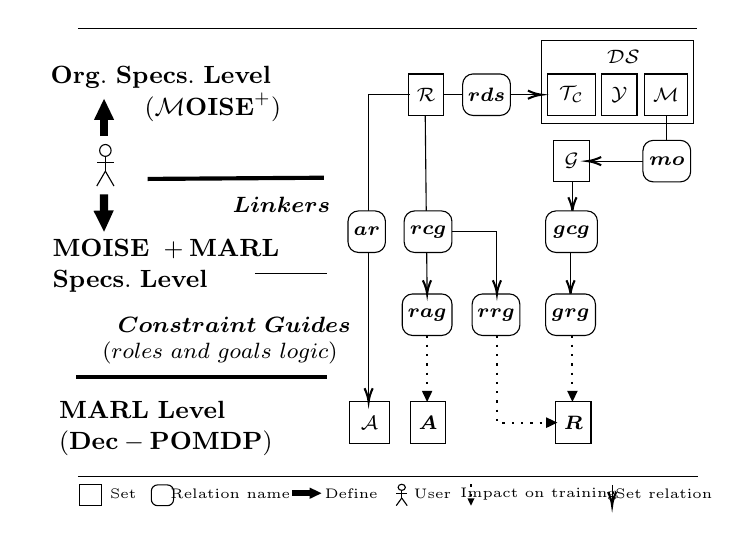
\begin{tikzpicture}[x=0.75pt,y=0.75pt,yscale=-1,xscale=1]
%uncomment if require: \path (0,2584); %set diagram left start at 0, and has height of 2584

%Straight Lines [id:da4973066741986565] 
\draw [line width=1.5]    (118.21,2302.58) -- (203.1,2302) ;
%Straight Lines [id:da14807114776731778] 
\draw    (368.35,2272) -- (368.35,2294) -- (332.16,2294) ;
\draw [shift={(330.16,2294)}, rotate = 360] [color={rgb, 255:red, 0; green, 0; blue, 0 }  ][line width=0.75]    (6.56,-1.97) .. controls (4.17,-0.84) and (1.99,-0.18) .. (0,0) .. controls (1.99,0.18) and (4.17,0.84) .. (6.56,1.97)   ;
%Straight Lines [id:da16285043353898754] 
\draw [line width=1.5]    (83.88,2398) -- (204.61,2398) ;
%Straight Lines [id:da6299512000169913] 
\draw    (169.94,2348) -- (204.61,2348) ;
%Straight Lines [id:da64750232417664] 
\draw    (84.65,2446) -- (383.15,2446) ;
%Straight Lines [id:da35895220906699743] 
\draw    (84.65,2230) -- (383,2230) ;
%Straight Lines [id:da715014372569708] 
\draw    (244.68,2262) -- (224.68,2262) -- (224.68,2408) ;
\draw [shift={(224.68,2410)}, rotate = 270] [color={rgb, 255:red, 0; green, 0; blue, 0 }  ][line width=0.75]    (6.56,-1.97) .. controls (4.17,-0.84) and (1.99,-0.18) .. (0,0) .. controls (1.99,0.18) and (4.17,0.84) .. (6.56,1.97)   ;
%Straight Lines [id:da71870438525014] 
\draw    (251.96,2328) -- (286.51,2328) -- (286.51,2356) ;
\draw [shift={(286.51,2358)}, rotate = 270] [color={rgb, 255:red, 0; green, 0; blue, 0 }  ][line width=0.75]    (6.56,-1.97) .. controls (4.17,-0.84) and (1.99,-0.18) .. (0,0) .. controls (1.99,0.18) and (4.17,0.84) .. (6.56,1.97)   ;
%Straight Lines [id:da6006267784187092] 
\draw [line width=0.75]  [dash pattern={on 0.84pt off 2.51pt}]  (252.87,2378) -- (252.87,2407) ;
\draw [shift={(252.87,2410)}, rotate = 270] [fill={rgb, 255:red, 0; green, 0; blue, 0 }  ][line width=0.08]  [draw opacity=0] (5.36,-2.57) -- (0,0) -- (5.36,2.57) -- cycle    ;
%Straight Lines [id:da8743336135156266] 
\draw    (322.88,2304) -- (322.88,2316) ;
\draw [shift={(322.88,2318)}, rotate = 270] [color={rgb, 255:red, 0; green, 0; blue, 0 }  ][line width=0.75]    (6.56,-1.97) .. controls (4.17,-0.84) and (1.99,-0.18) .. (0,0) .. controls (1.99,0.18) and (4.17,0.84) .. (6.56,1.97)   ;
%Straight Lines [id:da14641229967966152] 
\draw [line width=0.75]  [dash pattern={on 0.84pt off 2.51pt}]  (322.88,2378) -- (322.88,2407) ;
\draw [shift={(322.88,2410)}, rotate = 270] [fill={rgb, 255:red, 0; green, 0; blue, 0 }  ][line width=0.08]  [draw opacity=0] (5.36,-2.57) -- (0,0) -- (5.36,2.57) -- cycle    ;
%Straight Lines [id:da9260929933425808] 
\draw [line width=0.75]  [dash pattern={on 0.84pt off 2.51pt}]  (286.51,2378) -- (286.51,2420) -- (312.61,2420) ;
\draw [shift={(315.61,2420)}, rotate = 180] [fill={rgb, 255:red, 0; green, 0; blue, 0 }  ][line width=0.08]  [draw opacity=0] (5.36,-2.57) -- (0,0) -- (5.36,2.57) -- cycle    ;
%Straight Lines [id:da3057006030233673] 
\draw [line width=0.75]  [dash pattern={on 0.84pt off 2.51pt}]  (274,2449.7) -- (274,2457) ;
\draw [shift={(274,2460)}, rotate = 270] [fill={rgb, 255:red, 0; green, 0; blue, 0 }  ][line width=0.08]  [draw opacity=0] (3.57,-1.72) -- (0,0) -- (3.57,1.72) -- cycle    ;
%Straight Lines [id:da07288166228322246] 
\draw    (342,2449.98) -- (342,2458) ;
\draw [shift={(342,2460)}, rotate = 270] [color={rgb, 255:red, 0; green, 0; blue, 0 }  ][line width=0.75]    (6.56,-1.97) .. controls (4.17,-0.84) and (1.99,-0.18) .. (0,0) .. controls (1.99,0.18) and (4.17,0.84) .. (6.56,1.97)   ;
%Shape: Ellipse [id:dp8508274348425935] 
\draw   (95.09,2288.86) .. controls (95.09,2287.28) and (96.33,2286) .. (97.85,2286) .. controls (99.38,2286) and (100.62,2287.28) .. (100.62,2288.86) .. controls (100.62,2290.44) and (99.38,2291.71) .. (97.85,2291.71) .. controls (96.33,2291.71) and (95.09,2290.44) .. (95.09,2288.86) -- cycle ;
%Straight Lines [id:da3825450168053828] 
\draw    (97.85,2291.71) -- (97.85,2298.86) ;
%Straight Lines [id:da521321206042058] 
\draw    (97.85,2298.86) -- (93.71,2306) ;
%Straight Lines [id:da055514206493922025] 
\draw    (97.85,2298.86) -- (102,2306) ;
%Straight Lines [id:da8996496708356774] 
\draw    (102,2294.57) -- (93.71,2294.57) ;

%Straight Lines [id:da31678488015771755] 
\draw [line width=2.25]    (188,2454) -- (196.97,2454) ;
\draw [shift={(201.97,2454)}, rotate = 180] [fill={rgb, 255:red, 0; green, 0; blue, 0 }  ][line width=0.08]  [draw opacity=0] (5.72,-2.75) -- (0,0) -- (5.72,2.75) -- cycle    ;
%Shape: Ellipse [id:dp3927356466672782] 
\draw   (238.88,2451.17) .. controls (238.88,2450.36) and (239.67,2449.7) .. (240.64,2449.7) .. controls (241.61,2449.7) and (242.4,2450.36) .. (242.4,2451.17) .. controls (242.4,2451.99) and (241.61,2452.65) .. (240.64,2452.65) .. controls (239.67,2452.65) and (238.88,2451.99) .. (238.88,2451.17) -- cycle ;
%Straight Lines [id:da3365602555559104] 
\draw    (240.64,2452.65) -- (240.64,2456.32) ;
%Straight Lines [id:da7990875235744026] 
\draw    (240.64,2456.32) -- (238,2460) ;
%Straight Lines [id:da23945649338821617] 
\draw    (240.64,2456.32) -- (243.28,2460) ;
%Straight Lines [id:da11927353559661591] 
\draw    (243.28,2454.12) -- (238,2454.12) ;

%Straight Lines [id:da5816423191130675] 
\draw    (251.96,2272) -- (252.85,2356) ;
\draw [shift={(252.87,2358)}, rotate = 269.39] [color={rgb, 255:red, 0; green, 0; blue, 0 }  ][line width=0.75]    (6.56,-1.97) .. controls (4.17,-0.84) and (1.99,-0.18) .. (0,0) .. controls (1.99,0.18) and (4.17,0.84) .. (6.56,1.97)   ;
%Straight Lines [id:da9310455126832857] 
\draw    (321.97,2338) -- (321.97,2356) ;
\draw [shift={(321.97,2358)}, rotate = 270] [color={rgb, 255:red, 0; green, 0; blue, 0 }  ][line width=0.75]    (6.56,-1.97) .. controls (4.17,-0.84) and (1.99,-0.18) .. (0,0) .. controls (1.99,0.18) and (4.17,0.84) .. (6.56,1.97)   ;
%Shape: Rectangle [id:dp293492578719597] 
\draw   (120,2453) .. controls (120,2451.34) and (121.34,2450) .. (123,2450) -- (127.72,2450) .. controls (129.37,2450) and (130.72,2451.34) .. (130.72,2453) -- (130.72,2457) .. controls (130.72,2458.66) and (129.37,2460) .. (127.72,2460) -- (123,2460) .. controls (121.34,2460) and (120,2458.66) .. (120,2457) -- cycle ;
%Straight Lines [id:da33566712615128225] 
\draw    (261.05,2262) -- (306,2262) ;
\draw [shift={(308,2262)}, rotate = 180] [color={rgb, 255:red, 0; green, 0; blue, 0 }  ][line width=0.75]    (6.56,-1.97) .. controls (4.17,-0.84) and (1.99,-0.18) .. (0,0) .. controls (1.99,0.18) and (4.17,0.84) .. (6.56,1.97)   ;
%Shape: Rectangle [id:dp28383270948937667] 
\draw   (308,2236) -- (381.08,2236) -- (381.08,2276) -- (308,2276) -- cycle ;
%Straight Lines [id:da18020989903965012] 
\draw [line width=3]    (97.22,2282) -- (97.22,2270) ;
\draw [shift={(97.22,2264)}, rotate = 90] [fill={rgb, 255:red, 0; green, 0; blue, 0 }  ][line width=0.08]  [draw opacity=0] (10.18,-4.89) -- (0,0) -- (10.18,4.89) -- cycle    ;
%Straight Lines [id:da018421338049046554] 
\draw [line width=3]    (97.22,2310) -- (97.11,2322.37) ;
\draw [shift={(97.22,2328)}, rotate = 268.86] [fill={rgb, 255:red, 0; green, 0; blue, 0 }  ][line width=0.08]  [draw opacity=0] (10.18,-4.89) -- (0,0) -- (10.18,4.89) -- cycle    ;
%Shape: Rectangle [id:dp7281037051878541] 
\draw   (85.42,2450) -- (96.13,2450) -- (96.13,2460) -- (85.42,2460) -- cycle ;


% Text Node
\draw  [fill={rgb, 255:red, 255; green, 255; blue, 255 }  ,fill opacity=1 ]  (241.82,2323) .. controls (241.82,2320.24) and (244.06,2318) .. (246.82,2318) -- (259.82,2318) .. controls (262.58,2318) and (264.82,2320.24) .. (264.82,2323) -- (264.82,2333) .. controls (264.82,2335.76) and (262.58,2338) .. (259.82,2338) -- (246.82,2338) .. controls (244.06,2338) and (241.82,2335.76) .. (241.82,2333) -- cycle  ;
\draw (253.32,2328) node  [font=\scriptsize] [align=left] {$\displaystyle \boldsymbol{rcg}$};
% Text Node
\draw    (337,2252) -- (354,2252) -- (354,2272) -- (337,2272) -- cycle  ;
\draw (345.5,2262) node  [font=\scriptsize] [align=left] {$\displaystyle \mathcal{Y}$};
% Text Node
\draw    (311,2252) -- (334,2252) -- (334,2272) -- (311,2272) -- cycle  ;
\draw (322.5,2262) node  [font=\scriptsize] [align=left] {$\displaystyle \mathcal{T_{C}}$};
% Text Node
\draw    (357.39,2252) -- (378.39,2252) -- (378.39,2272) -- (357.39,2272) -- cycle  ;
\draw (367.89,2262) node  [font=\scriptsize] [align=left] {$\displaystyle \mathcal{M}$};
% Text Node
\draw (347.43,2244) node  [font=\scriptsize] [align=left] {$\displaystyle \mathcal{DS}$};
% Text Node
\draw  [fill={rgb, 255:red, 255; green, 255; blue, 255 }  ,fill opacity=1 ]  (270,2257) .. controls (270,2254.24) and (272.24,2252) .. (275,2252) -- (288,2252) .. controls (290.76,2252) and (293,2254.24) .. (293,2257) -- (293,2267) .. controls (293,2269.76) and (290.76,2272) .. (288,2272) -- (275,2272) .. controls (272.24,2272) and (270,2269.76) .. (270,2267) -- cycle  ;
\draw (281.5,2262) node  [font=\scriptsize] [align=left] {$\displaystyle \boldsymbol{rds}$};
% Text Node
\draw (158,2454.5) node  [font=\tiny] [align=left] {Relation name};
% Text Node
\draw (106.46,2454.5) node  [font=\tiny] [align=left] {Set};
% Text Node
\draw (255.47,2454.5) node  [font=\tiny] [align=left] {User};
% Text Node
\draw (216.32,2454.5) node  [font=\tiny] [align=left] {Define};
% Text Node
\draw (366.91,2454.5) node  [font=\tiny] [align=left] {Set relation};
% Text Node
\draw (306.61,2454.5) node  [font=\tiny] [align=left] {Impact on training};
% Text Node
\draw    (244.82,2410) -- (261.82,2410) -- (261.82,2430) -- (244.82,2430) -- cycle  ;
\draw (253.32,2420) node  [font=\scriptsize] [align=left] {$\displaystyle \boldsymbol{A}$};
% Text Node
\draw    (314.84,2410) -- (331.84,2410) -- (331.84,2430) -- (314.84,2430) -- cycle  ;
\draw (323.34,2420) node  [font=\scriptsize] [align=left] {$\displaystyle \boldsymbol{R}$};
% Text Node
\draw    (215.63,2410) -- (234.63,2410) -- (234.63,2430) -- (215.63,2430) -- cycle  ;
\draw (225.13,2420) node  [font=\scriptsize] [align=left] {$\displaystyle \mathcal{A}$};
% Text Node
\draw  [fill={rgb, 255:red, 255; green, 255; blue, 255 }  ,fill opacity=1 ]  (309.97,2363) .. controls (309.97,2360.24) and (312.21,2358) .. (314.97,2358) -- (328.97,2358) .. controls (331.73,2358) and (333.97,2360.24) .. (333.97,2363) -- (333.97,2373) .. controls (333.97,2375.76) and (331.73,2378) .. (328.97,2378) -- (314.97,2378) .. controls (312.21,2378) and (309.97,2375.76) .. (309.97,2373) -- cycle  ;
\draw (321.97,2368) node  [font=\scriptsize] [align=left] {$\displaystyle \boldsymbol{grg}$};
% Text Node
\draw    (274.56,2363) .. controls (274.56,2360.24) and (276.8,2358) .. (279.56,2358) -- (292.56,2358) .. controls (295.32,2358) and (297.56,2360.24) .. (297.56,2363) -- (297.56,2373) .. controls (297.56,2375.76) and (295.32,2378) .. (292.56,2378) -- (279.56,2378) .. controls (276.8,2378) and (274.56,2375.76) .. (274.56,2373) -- cycle  ;
\draw (286.06,2368) node  [font=\scriptsize] [align=left] {$\displaystyle \boldsymbol{rrg}$};
% Text Node
\draw    (240.87,2363) .. controls (240.87,2360.24) and (243.11,2358) .. (245.87,2358) -- (259.87,2358) .. controls (262.63,2358) and (264.87,2360.24) .. (264.87,2363) -- (264.87,2373) .. controls (264.87,2375.76) and (262.63,2378) .. (259.87,2378) -- (245.87,2378) .. controls (243.11,2378) and (240.87,2375.76) .. (240.87,2373) -- cycle  ;
\draw (252.87,2368) node  [font=\scriptsize] [align=left] {$\displaystyle \boldsymbol{rag}$};
% Text Node
\draw (156.15,2380.5) node  [font=\footnotesize] [align=left] {$\displaystyle  \begin{array}{{>{\displaystyle}l}}
\ \ \boldsymbol{Constraint\ Guides}\\
( roles\ and\ goals\ logic)
\end{array}$};
% Text Node
\draw  [fill={rgb, 255:red, 255; green, 255; blue, 255 }  ,fill opacity=1 ]  (309.93,2323) .. controls (309.93,2320.24) and (312.17,2318) .. (314.93,2318) -- (329.93,2318) .. controls (332.69,2318) and (334.93,2320.24) .. (334.93,2323) -- (334.93,2333) .. controls (334.93,2335.76) and (332.69,2338) .. (329.93,2338) -- (314.93,2338) .. controls (312.17,2338) and (309.93,2335.76) .. (309.93,2333) -- cycle  ;
\draw (322.43,2328) node  [font=\scriptsize] [align=left] {$\displaystyle \boldsymbol{gcg}$};
% Text Node
\draw  [fill={rgb, 255:red, 255; green, 255; blue, 255 }  ,fill opacity=1 ]  (214.77,2323) .. controls (214.77,2320.24) and (217.01,2318) .. (219.77,2318) -- (227.77,2318) .. controls (230.53,2318) and (232.77,2320.24) .. (232.77,2323) -- (232.77,2333) .. controls (232.77,2335.76) and (230.53,2338) .. (227.77,2338) -- (219.77,2338) .. controls (217.01,2338) and (214.77,2335.76) .. (214.77,2333) -- cycle  ;
\draw (223.77,2328) node  [font=\scriptsize] [align=left] {$\displaystyle \boldsymbol{ar}$};
% Text Node
\draw  [fill={rgb, 255:red, 255; green, 255; blue, 255 }  ,fill opacity=1 ]  (356.85,2289) .. controls (356.85,2286.24) and (359.08,2284) .. (361.85,2284) -- (374.85,2284) .. controls (377.61,2284) and (379.85,2286.24) .. (379.85,2289) -- (379.85,2299) .. controls (379.85,2301.76) and (377.61,2304) .. (374.85,2304) -- (361.85,2304) .. controls (359.08,2304) and (356.85,2301.76) .. (356.85,2299) -- cycle  ;
\draw (368.35,2294) node  [font=\scriptsize] [align=left] {$\displaystyle \boldsymbol{mo}$};
% Text Node
\draw (127,2344.5) node  [font=\small] [align=left] {$\displaystyle  \begin{array}{{>{\displaystyle}l}}
\mathbf{MOISE\ +MARL}\\
\mathbf{Specs.\ Level}
\end{array}$};
% Text Node
\draw (127,2422.5) node  [font=\small] [align=left] {$\displaystyle  \begin{array}{{>{\displaystyle}l}}
\mathbf{MARL\ Level}\\
\mathbf{( Dec-POMDP)}
\end{array}$};
% Text Node
\draw    (243.91,2252) -- (260.91,2252) -- (260.91,2272) -- (243.91,2272) -- cycle  ;
\draw (252.41,2262) node  [font=\scriptsize] [align=left] {$\displaystyle \mathcal{R}$};
% Text Node
\draw (182.64,2315) node  [font=\footnotesize] [align=left] {$\displaystyle \boldsymbol{Linkers}$};
% Text Node
\draw    (313.93,2284) -- (330.93,2284) -- (330.93,2304) -- (313.93,2304) -- cycle  ;
\draw (322.43,2294) node  [font=\scriptsize] [align=left] {$\displaystyle \mathcal{G}$};
% Text Node
\draw (127,2261.5) node  [font=\small] [align=left] {$\displaystyle  \begin{array}{{>{\displaystyle}l}}
\mathbf{{\displaystyle Org.\ Specs.\ Level}}\\
{\displaystyle \ \ \ \ \ \ \ \ \ \ \ (\mathcal{M}\mathbf{OISE^+})}
\end{array}$};


\end{tikzpicture}
    \caption{A minimal view of the MOISE+MARL framework.}
    \label{fig:mm_synthesis}
\end{figure}


\noindent MOISE+MARL introduces means to control or guide the agents' training in MARL. Within this framework, \textbf{agents are not fully manually programmed}; instead, their policies are learned under organizational constraints by changing their action space (shielding~\cite{alshiekh2018safe}) to encode hard constraints captured within the notion of roles, or the reward function (reward shaping~\cite{marom2018belief}) to encode soft constraints captured within the notion of goals. These roles and goals are defined as sets of "rules" enabling to integrate any expert knowledge such as a predefined agent architecture.

It is worth noting that we assume the environment excludes agents: agents are autonomous decision-makers interacting via observations and actions. The $\mathcal{M}OISE^+$ specification is a design-time, symbolic layer used to (i) guide training (e.g., action masking or reward shaping) and (ii) interpret learned policies; deployed systems need not implement or be bound by $\mathcal{M}OISE^+$ at runtime.
The MOISE+MARL core contribution are the \textbf{Constraint Guides}, which are the three new relations introduced to describe the logic of roles and goals in the decentralized partially observable Markov decision process formalism:
%
\begin{enumerate*}[label={\roman*) },itemjoin={; \quad}]
    
    \item \textbf{Role Action Guide} \quad $rag: H \times \Omega \rightarrow \mathcal{P}(A \times \mathbb{R})$, the relation that models a role as a set of rules which, for each pair consisting of a history $h \in H$ and an observation $\omega \in \Omega$ received by the agent, associates each expected actions in $A \in \mathcal{P}(A)$ with a constraint hardness $ch \in [0,1]$ ($ch = 1$ by default). By restricting the choice of the next action among those authorized, the agent is forced to adhere to the role's expected behavior
    \item \textbf{Role Reward Guide} \quad $rrg: H \times \Omega \times A \to \mathbb{R} = \{r_m \text{ if } a \notin A_\omega \text{, } rag(h, \omega) \allowbreak = \allowbreak A_\omega \times \mathbb{R} \text{, } h \in H; \text{ else } 0\}$, the relation that models a role by adding a penalty $r_m$ to the global reward if the last action chosen by the agent $a \in A$ is not authorized. This is intended to encourage the agent to adhere to the expected behavior
    \item \textbf{Goal Reward Guide} \quad $grg: H \rightarrow \mathbb{R}$, the relation that models a goal as a soft constraint adding a reward bonus $r_b \in \mathbb{R}$ if the agent's history $h \in H$ contains a goal's characteristic sub-sequence $h_g \in H_g$, encouraging the agent to reach it.
\end{enumerate*}

\noindent Finally, we introduce the \textbf{Linkers} to link the $\mathcal{M}OISE^+$ organizational specifications with constraint guides and agents:
%
\begin{enumerate*}[label={\roman*) },itemjoin={; \quad}]
    
    \item \textbf{Agent to Role} \quad $ar: \mathcal{A} \to \mathcal{R}$, the bijective relation linking an agent to a role
    \item \textbf{Role to Constraint Guide} \quad $rcg: \mathcal{R} \rightarrow rag \cup rrg$, the relation associating each $\mathcal{M}OISE^+$ role to a $rag$ or $rrg$ relation, forcing/encouraging the agent to follow the expected actions for the role $\rho \in \mathcal{R}$
    \item \textbf{Goal to Constraint Guide} \quad $gcg: \mathcal{G} \rightarrow grg$, the relation linking goals to $grg$ relations, representing goals as rewards in MARL.
\end{enumerate*}

\paragraph*{\textbf{Facilitating the implementation of Constraint Guides}}

Roles, missions and goals are only labels; defining \(rag/rrg/grg\) extensionally requires large, redundant history sets and does not scale. Constraint Guides therefore decide, from a history \(h\), whether \(h\) matches an expected behavior and what to enforce (action masking or reward shaping). A procedural option uses predicates \(b_g: H \to \{0,1\}\) (e.g., Python rules), which is flexible but verbose and hard to maintain. We introduce Trajectory-based Patterns (TPs): compact declarative temporal patterns \(p\in P\) that match families of histories after mapping observations/actions to labels \(l:\Omega\cup A\to L\), making patterns concise and environment-agnostic.\\

\noindent \textbf{Concrete example: } Consider the \textit{Overcooked-AI}~\cite{overcookedai} environment, where chef agents must collaborate by moving around a grid world and interacting with ingredients (onions) and instruments (pots, bowls) to make soup, which is shipped by interacting with the shipping area. Here, we want to recognize the following behavior: \textquote{an agent who holds an onion observes a pot and interacts with it to fill it}. This behavior can be expressed by the following TP:
\[
    p = [[\#any](*) , \; has_onion , \; [\#any](*) , \; see_pot , \; interact \;](1,1)
\]

\noindent
This TP means an agent may have done some previous unknown actions, but at some point it has an onion. Then it can do some unknown actions before seeing a pot and interacting with it immediately after. This TP can be used within constraint guides as shown in \autoref{tab:tp_guides_example} to encourage the agent to interact again to retrieve the soup, for example.

\begin{table}[h]
    \centering
    \caption{Examples of guides applied to the TP "fill a pot with an onion".}
    \label{tab:tp_guides_example}
    \scriptsize
    \renewcommand{\arraystretch}{1.3}
    % \setlength{\tabcolsep}{10pt}
    \begin{tabular}{p{4cm}@{\hspace{20pt}}p{8cm}}
        \hline
        \textbf{Guide}                            & \textbf{Example rule}                                    \\
        \hline
        \textbf{RAG} (\textit{Role Action Guide}) & If the TP is satisfied, restrict possible actions~:
        \[
            rag(h,\omega) = \{\texttt{interact} \mapsto 1.0, \;\texttt{nothing} \mapsto 0.2\}
        \]
        The action \texttt{interact} is strongly favored.                                                    \\
        
        \hline
        
        \textbf{RRG} (\textit{Role Reward Guide}) & Add a role bonus when the expected action is performed~:
        \[
            rrg(h,\omega,a) =
            \begin
            {cases}
        +3                                        & \text{if } a = \text{interact}                           \\
        0                                         & \text{otherwise}
            \end{cases}
        \]                                                                                                   \\
        \hline
        
        \textbf{GRG} (\text{Goal Reward Guide})   & Grant a reward if the TP is detected/achieved:
        \[
            grg(h) =
            \begin{cases}
                +5 & \text{if the pot is full (TP recognized)} \\
                0  & \text{otherwise}
            \end{cases}
        \]                                                                                                   \\
        \hline
    \end{tabular}
\end{table}

Thus, instead of extensionally defining vast sets \(H_g\), the user describes a few symbolic patterns that capture the essence of the desired behaviors. MOISE+MARL then automatically applies these patterns to the guides (\(rag, rrg, grg\)), making their implementation more modular, scalable, and interpretable.

\paragraph*{\textbf{Resolving the Dec-POMDP with MOISE+MARL}}

A MOISE+MARL model is defined as $\mathcal{MM} = \langle \mathcal{OS}, ar, rcg, gcg, rag, rrg, grg \rangle$.
Solving a Dec-POMDP with $mm \in \mathcal{MM}$ consists in finding a joint policy $\pi^j = {\pi^j_0, \pi^j_1, \dots, \pi^j_n}$ that maximizes the expected cumulative reward (or satisfies a minimal threshold), represented by the state-value function $V^{\pi^j}$. This value reflects the return from an initial state $s \in S$ when applying successive joint actions $a^j \in A^n$ under the additional organizational constraints.
%
The definition of $V^{\pi^j}$ follows the sequential and cyclic agent execution scheme (AEC mode), and is formalized in \hyperref[eq:single_value_function]{Definition 1}, incorporating role-based (in \textcolor{red}{red}) and mission-based (in \textcolor{blue}{blue}) adaptations that influence both the action space and the reward.
\autoref{fig:mm_synthesis} summarizes the MOISE+MARL instantiation: given an organizational specification \(\mathcal{OS}=\langle\mathcal{R},\mathcal{M},mo,\mathcal{G},\mathcal{PER},\mathcal{OBL}\rangle\) we form \(\mathcal{MM}=\langle\mathcal{OS},ar,rcg,gcg,rag,rrg,grg\rangle\) with \(ar:\mathcal{A}\to\mathcal{R},\;rcg:\mathcal{R}\to\{rag,rrg\},\;gcg:\mathcal{G}\to\{grg\}\); \(rag(h,\omega)\subseteq A\) gives role-authorized actions, \(rrg(h,\omega,a)\in\mathbb{R}\) is a penalty for unauthorized actions, \(grg(h)\in\mathbb{R}\) is a goal bonus, and a hardness parameter \(ch\in[0,1]\) controls enforcement (action masking if \(ch=1\), penalization if \(ch<1\)). Operationally, agents are mapped to roles via \(ar\), \(rag\) is compiled into action masks and \(rrg,grg\) into additive reward modifiers, and MARL (CTDE-compatible) optimizes the resulting (O)Dec‑POMDP using masked action sets and the shaped reward, yielding a single constrained optimization: maximize the expected cumulative shaped return under \(\mathcal{MM}\).

\medskip


\begin{figure*}[h!]
    \label{eq:single_value_function}
    \raggedright
    \textbf{\textit{Definition 2} \quad Observation-Value function adapted to constraint guides in parallel mode:}
    
    \begin{scriptsize}
        \vspace{-0.6cm}
        \begin{gather*}
            V^{\pi^j}(\tilde{h}_{t-1},h^j_{t-1},\hat{\omega}^j_t) = \hspace{-0.95cm}
            %
            \sum_{\textcolor{red}{ \substack{a^j_{t} \in A^j \text{ if } rn() < ch_{t}, \\
            a^j_{t} \in A^j_{t} \text{ else}}
            }}{\hspace{-0.9cm} \pi_i(a^j_{t} | \hat{\omega}^j_t)}
            %
            \hspace{-1.2cm}
            \sum_{\phantom{XXXX}(\tilde{h}_t,\hat{\omega}^j_{t+1}) \in \mathcal{H} \times \hat{\Omega}^j}
            %
            {\hspace{-1.2cm} \mathcal{T}^j(\langle \tilde{h}_t,\hat{\omega}^j_{t+1} \rangle | \tilde{h}_{t-1}, \hat{\omega}_t, a^j_{t})
            \Bigl[R^j_H(h^j_{t-1},\hat{\omega}^j_t,a^j_t,\hat{\omega}^j_{t+1}) \hspace{-0.1cm} }
        \end{gather*}
        %
        \vspace{-1cm}
        \begin{gather*}
            \hspace{3.6cm}
            {+ \  \textcolor{blue}{grg^j_m(h^j_t)}
            +
            \textcolor{red}{(1-ch_t) \times rrg^j(h^j_{t-1},\hat{\omega}^j_t,a^j_{t+1})} + V^{\pi^j}(\tilde{h}_{t}, h^j_t, \hat{\omega}^j_{t+1})\Bigr]}
        \end{gather*}
        %
        \vspace{-0.15cm}
        %
        \[\hspace{-0.9cm}\text{With \ } \tilde{h}_{-1} = \mathbf{0} \text{ and } \tilde{\omega}^j_0 \in \Omega_0^{\mathcal{T}^j} \text{ ; } a^j_t = \langle a_{t,0}, a_{t,1} \dots a_{t,|\mathcal{A}|} \rangle \text{ ; } \omega^j_t = \langle \omega_{t,0}, \omega_{t,1} \dots \omega_{t,|\mathcal{A}|} \rangle \text{ ; }\]
        %
        \vspace{-0.25cm}
        \[\hspace{-5.85cm} h^j_t = \langle h_{t,0}, h_{t,1} \dots h_{t,|\mathcal{A}|} \rangle = \langle \langle h_{t-1,i}, \omega_{t,i}, a_{t,i} \rangle \rangle_{i \in \mathcal{A}}\]
        %
        \vspace{-0.2cm}
        \textcolor{red}{\[\hspace{-2.6cm}\text{ \hspace{-0.1cm} With } \langle rag_i, rrg_i \rangle = rcg(ar(i)) \text{ ; } rn: \emptyset \to [0,1[ \text{, a uniform random function}\]}
        %
        \vspace{-0.3cm}
        \textcolor{red}{\[A^j_t \times \mathbf{R}^{|\mathcal{A}|} \hspace{-0.1cm} = \hspace{-0.1cm} rag^j(h^j_t, \tilde{\omega}^j_t) \hspace{-0.1cm} = \hspace{-0.1cm} \langle rag_i(h_{t,i}, \omega_{t,i}) \rangle_{i \in \mathcal{A}} \text{ ; } rrg^j(h^j_{t-1}, \tilde{\omega}^j_t, a^j_t) \hspace{-0.1cm} = \hspace{-0.1cm} \sum_{i \in \mathcal{A}}{rrg_i(h_{t-1,i}, \omega_{t,i}, a_{t,i})}\]}
        %
        \vspace{-0.75cm}
        \textcolor{blue}{
            \begin{gather*}
                \hspace{-1.7cm} grg_m(h) = \hspace{-1cm} \sum_{\hspace{0.3cm}(grg_i,w_i) \in mo(m)}{\hspace{-1.1cm} w_i \times grg_i(h)}
                \text{ ; }
                grg^j_m(h^j_t) = \hspace{-0.1cm} \sum_{i \in \mathcal{A}}{\sum_{m \in \mathcal{M}_i}{ \hspace{-0.1cm} v_m(t) \frac{grg_m(h_{t,i})}{1 - p + \epsilon} }} \text{ ; } \epsilon \in \mathbb{R}_{>0} \text{ ; }
            \end{gather*}
        }
        \vspace{-0.9cm}
        \textcolor{blue}{
            \begin{gather*}
                \hspace{-4cm}
                v_m(t) = \{ 1 \text{ if } t \in t_c \text{ ; else } 0 \} \text{ ; } \mathcal{M}_i = \{m_j | \langle ar(i),m_j,t_c,p \rangle \in \mathcal{M}\}
            \end{gather*}
        }
    \end{scriptsize}
    
\end{figure*}

\noindent At each time step $t \in \mathbb{N}$ (starting from $t=0$), agent $i = t \bmod n$ is assigned to role $\rho_i = ar(i)$. For each temporally valid deontic specification $d_i = rds(\rho_i) = \langle tc_i, y_i, m_i \rangle$, the agent is permitted ($y_i = 0$) or obligated ($y_i = 1$) to commit to mission $m_i \in \mathcal{M}$, with goal set $\mathcal{G}_{m_i} = mo(m_i)$ and $n \in \mathbb{N}$ agents.
%
Upon observing $\omega_t$, agent $i$ samples its action according to its 
policy $\pi_i(a_t \mid \omega_t)$, which denotes the conditional 
probability of selecting action $a_t \in A_t$ given the current observation 
$\omega_t \in \Omega_t$. The agent selects an action $a_t$ from $A_t$ (the role-expected actions) with probability $ch_t$ (or from $A$ otherwise). Consequently, if $ch_t = 1$, the agent is strictly constrained by its role (which is the default value).
%
The selected action transitions the system from $s_t$ to $s_{t+1}$, yields observation $\omega_{t+1}$, and returns a reward composed of:
i) bonuses for achieved goals in valid missions (via Goal Reward Guides), weighted by $\frac{1}{1 - p + \epsilon}$. $v_m(t)$ indicates whether the time constraint associated with mission $m$ (by default $t_c = \mathbb{N}$) is still active at time $t$ ($v_m(t)=1$ while the mission's time-to-live has not expired and $v_m(t)=0$ otherwise so that the mission reward is no longer counted);
ii) penalties from the Role Reward Guide, scaled by $ch_t$.
%
The process continues in state $s_{t+1}$ with agent $(i + 1) \bmod n$.

\subsection{The TEMM method}
\label{sec:TEMM_algorithm}

The TEMM method is part of the explanation component of the MOISE+MARL framework. It leverages unsupervised learning techniques to infer organizational specifications from observed agent trajectories. It allows computing the organizational fit which is introduced theoretically as a quantitative indicator that we theorize and that ranges from 0 to 1 to assess the extent to which agents' behaviors are structured and compliant with organizational specifications. Those organizational specifications can be explicitly defined by users or implicit in that sense they are to be inferred via the TEMM method itself. A value close to 1 indicates that agents adopt regular, stable behaviors that are strongly aligned with a defined organization. Conversely, a value close to 0 means that behaviors are highly irregular and that no coherent organizational pattern emerges. In summary, organizational fit assesses the conformity of a joint policy to a structured and functional organization.

\textbf{1) Roles and role inheritance.} \quad TEMM defines a role $\rho$ as a policy whose agents share a \textit{Common Longest Sequence} (CLS) in their histories. A role $\rho_2$ inherits from $\rho_1$ if $\text{CLS}(\rho_2) \subseteq \text{CLS}(\rho_1)$. Hierarchical clustering is used to extract these CLSs and role hierarchies from trajectories. The \textbf{structural organizational fit} is computed as the distance between actual agent behaviors and inferred role sequences.

\textbf{2) Goals, plans, and missions.} \quad Goals are identified as clusters of joint-observations commonly reached in successful trajectories, using K-means over trajectory embeddings. Plans are inferred as sub-sequences of transitions that consistently lead to goals. A \textbf{mission} groups goals pursued collectively by one or more agents. The \textbf{functional organizational fit} quantifies how well current behaviors match inferred goals and missions.

\textbf{3) Permissions and obligations.} \quad In scenarios where organizational constraints are predefined, permissions and obligations are explicitly encoded in the MOISE+ specification and enforced during training. In contrast, when no normative structure is specified by the designer, permissions and obligations are \emph{inferred} from execution traces through Auto-TEMM: agents fulfilling a role are examined to determine whether they consistently (or exclusively) achieve particular missions under temporal constraints. Obligations imply exclusivity, whereas permissions imply optionality. The global \textbf{organizational fit} aggregates structural and functional scores derived from these normative assessments.

While clustering hyperparameters may require manual tuning to ensure robust role and goal extraction, TEMM offers a principled way to analyze emergent organizational behaviors and refine specifications accordingly.



\subsection{Learning World Models}

In \textbf{RL}, and in particular in the context of partial observability, \textbf{world models}~\cite{ha2018recurrent, hafner2020dream} or \textit{World Models}\index{World Model} aim to learn internal models that approximate both the dynamics of the transition function and the observation function jointly. \textit{World Models} enable agents to perform planning, improve sampling efficiency, and facilitate safe exploration by allowing the agent to simulate future scenarios. This approach belongs to the \textbf{MBRL} ~\cite{moerland2020model} paradigm and is particularly useful for automatically constructing high-fidelity simulation models even in the absence of an explicit representation of the environment.

Formally, at each time step $t$, we denote $\omega_t \in \Omega$ as the current observation, $a_t \in A$ as the action performed, and $\tilde{h}_{t-1} \in \mathcal{H}$ as the recurrent hidden state summarizing the interaction history up to $t-1$. Since observations are generally high-dimensional (e.g., images or complex state vectors), an encoder $Enc: \Omega \rightarrow Z$ is applied to project the observations into a compact latent space $Z$, with $z_t = Enc(\omega_t)$, where $\dim(Z) \ll \dim(\Omega)$.

The main temporal structure is modeled using a \textbf{Recurrent Latent Dynamic Model (\textbf{RLDM})}~\cite{hafner2020dream} $\mathcal{T}^{z} = f(g(h_{t-1}, z_t, a_t))$, which predicts the next latent state $\hat{z}_{t+1}$ by updating the recurrent state via $f$ and applying latent dynamics via $g$~:
\[
    h_t = f(h_{t-1}, z_t, a_t), \quad \hat{z}_{t+1} = g(h_t)
\]
where $f(\cdot)$ typically corresponds to a recurrent neural network \textbf{RNN}\index{RNN} (e.g., an \textbf{LSTM}~\cite{hochreiter1997long}\index{LSTM}) applied to the concatenation of $h_{t-1} $, $z_t$ and $a_t$, and $g(\cdot)$ is a function (often implemented by an Multi-Layer Perceptron -- \textbf{MLP}) mapping the recurrent state to the latent representation of the next observation.

The predicted latent state is then decoded by $Dec: Z \rightarrow \Omega$ to produce the predicted observation $\hat{\omega}_{t+1} = Dec(\hat{z}_{t+1})$. The entire model is trained jointly to minimize both the \emph{reconstruction loss} $\|\omega_{t+1} - \hat{\omega}_{t+1}\|$ in the observation space, and optionally a latent prediction loss to stabilize the learning of the latent dynamics.

The recurrent hidden state $\tilde{h}_t$ acts as a compact summary of the complete interaction history up to time $t$, thus avoiding the need to explicitly store long observation-action sequences.

For the sake of brevity, we define the complete composition that directly associates the current observation, action, and recurrent state with the next predicted observation in the form of the Observation Prediction Model (\textbf{OPM})\index{Observation Prediction Model (OPM)}~:
\[
    \mathcal{T}(h_{t-1}, \omega_t, a_t)~:= Dec(g(f(h_{t-1}, Enc(\omega_t), a_t))) = \hat{\omega}_{t+1}.
\]

\begin{figure}[h!]
    \centering
    \resizebox{\textwidth}{!}{%
        


\tikzset{every picture/.style={line width=0.75pt}} %set default line width to 0.75pt        

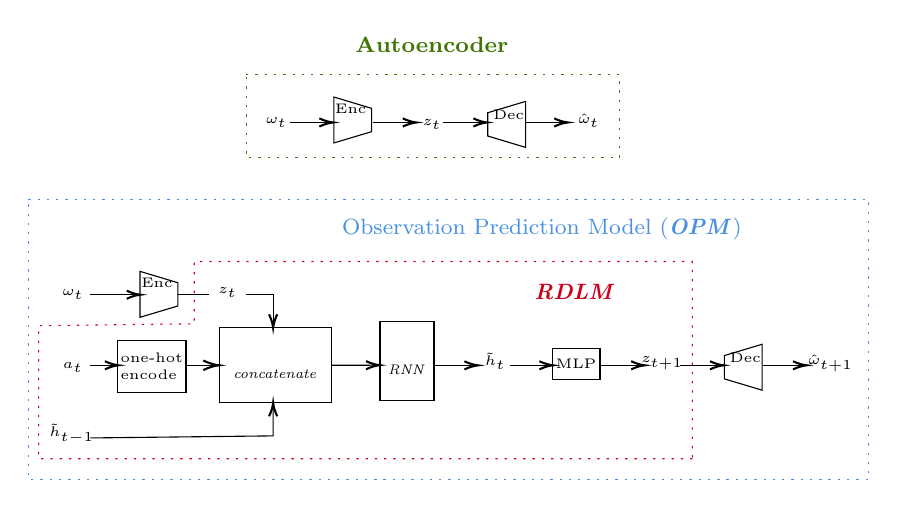
\begin{tikzpicture}[x=0.75pt,y=0.75pt,yscale=-1,xscale=1]
    %uncomment if require: \path (0,2102); %set diagram left start at 0, and has height of 2102

    %Straight Lines [id:da7945271061326031] 
    \draw    (100,1800) -- (111.5,1800) ;
    \draw [shift={(113.5,1800)}, rotate = 180] [color={rgb, 255:red, 0; green, 0; blue, 0 }  ][line width=0.75]    (6.56,-1.97) .. controls (4.17,-0.84) and (1.99,-0.18) .. (0,0) .. controls (1.99,0.18) and (4.17,0.84) .. (6.56,1.97)   ;
    %Straight Lines [id:da710289636295716] 
    \draw    (100,1835) -- (188,1834) -- (188,1820) ;
    \draw [shift={(188,1818)}, rotate = 90] [color={rgb, 255:red, 0; green, 0; blue, 0 }  ][line width=0.75]    (6.56,-1.97) .. controls (4.17,-0.84) and (1.99,-0.18) .. (0,0) .. controls (1.99,0.18) and (4.17,0.84) .. (6.56,1.97)   ;
    %Straight Lines [id:da9775676154282154] 
    \draw    (146.38,1800) -- (160,1800) ;
    \draw [shift={(162,1800)}, rotate = 180] [color={rgb, 255:red, 0; green, 0; blue, 0 }  ][line width=0.75]    (7.65,-2.3) .. controls (4.86,-0.97) and (2.31,-0.21) .. (0,0) .. controls (2.31,0.21) and (4.86,0.98) .. (7.65,2.3)   ;
    %Straight Lines [id:da789934339782699] 
    \draw    (100,1766) -- (122,1766) ;
    \draw [shift={(124,1766)}, rotate = 180] [color={rgb, 255:red, 0; green, 0; blue, 0 }  ][line width=0.75]    (6.56,-1.97) .. controls (4.17,-0.84) and (1.99,-0.18) .. (0,0) .. controls (1.99,0.18) and (4.17,0.84) .. (6.56,1.97)   ;
    %Shape: Trapezoid [id:dp2317709974845179] 
    \draw   (123.84,1754.74) -- (142.07,1760.21) -- (142.07,1771.42) -- (123.84,1776.88) -- cycle ;
    %Straight Lines [id:da7383754609221514] 
    \draw    (142,1766) -- (188,1766) -- (188,1780) ;
    \draw [shift={(188,1782)}, rotate = 270] [color={rgb, 255:red, 0; green, 0; blue, 0 }  ][line width=0.75]    (6.56,-1.97) .. controls (4.17,-0.84) and (1.99,-0.18) .. (0,0) .. controls (1.99,0.18) and (4.17,0.84) .. (6.56,1.97)   ;
    %Straight Lines [id:da49394763541143527] 
    \draw    (216,1800) -- (237.33,1799.94) ;
    \draw [shift={(239.33,1799.94)}, rotate = 179.85] [color={rgb, 255:red, 0; green, 0; blue, 0 }  ][line width=0.75]    (6.56,-1.97) .. controls (4.17,-0.84) and (1.99,-0.18) .. (0,0) .. controls (1.99,0.18) and (4.17,0.84) .. (6.56,1.97)   ;
    %Straight Lines [id:da8738633046359771] 
    \draw    (265.89,1800.03) -- (284.72,1800.03) ;
    \draw [shift={(286.72,1800.03)}, rotate = 180] [color={rgb, 255:red, 0; green, 0; blue, 0 }  ][line width=0.75]    (6.56,-1.97) .. controls (4.17,-0.84) and (1.99,-0.18) .. (0,0) .. controls (1.99,0.18) and (4.17,0.84) .. (6.56,1.97)   ;
    %Straight Lines [id:da3021616845453272] 
    \draw    (302,1800) -- (320.83,1800) ;
    \draw [shift={(322.83,1800)}, rotate = 180] [color={rgb, 255:red, 0; green, 0; blue, 0 }  ][line width=0.75]    (6.56,-1.97) .. controls (4.17,-0.84) and (1.99,-0.18) .. (0,0) .. controls (1.99,0.18) and (4.17,0.84) .. (6.56,1.97)   ;
    %Straight Lines [id:da8984410115217915] 
    \draw    (346,1800) -- (353.4,1800) -- (365.04,1800) ;
    \draw [shift={(367.04,1800)}, rotate = 180] [color={rgb, 255:red, 0; green, 0; blue, 0 }  ][line width=0.75]    (6.56,-1.97) .. controls (4.17,-0.84) and (1.99,-0.18) .. (0,0) .. controls (1.99,0.18) and (4.17,0.84) .. (6.56,1.97)   ;
    %Shape: Trapezoid [id:dp37639710819638017] 
    \draw   (423.61,1812) -- (405.38,1806.53) -- (405.38,1795.32) -- (423.61,1789.86) -- cycle ;
    %Straight Lines [id:da10289425963982124] 
    \draw    (384,1800) -- (403.04,1800) ;
    \draw [shift={(405.04,1800)}, rotate = 180] [color={rgb, 255:red, 0; green, 0; blue, 0 }  ][line width=0.75]    (6.56,-1.97) .. controls (4.17,-0.84) and (1.99,-0.18) .. (0,0) .. controls (1.99,0.18) and (4.17,0.84) .. (6.56,1.97)   ;
    %Straight Lines [id:da12692360321469986] 
    \draw    (424,1800) -- (443.04,1800) ;
    \draw [shift={(445.04,1800)}, rotate = 180] [color={rgb, 255:red, 0; green, 0; blue, 0 }  ][line width=0.75]    (6.56,-1.97) .. controls (4.17,-0.84) and (1.99,-0.18) .. (0,0) .. controls (1.99,0.18) and (4.17,0.84) .. (6.56,1.97)   ;
    %Shape: Trapezoid [id:dp27180057752038367] 
    \draw   (217.23,1670.74) -- (235.46,1676.21) -- (235.46,1687.42) -- (217.23,1692.88) -- cycle ;
    %Shape: Trapezoid [id:dp9437628483591106] 
    \draw   (309.61,1695) -- (291.38,1689.53) -- (291.38,1678.32) -- (309.61,1672.86) -- cycle ;
    %Straight Lines [id:da19635385567867214] 
    \draw    (310,1683) -- (328,1683) ;
    \draw [shift={(330,1683)}, rotate = 180] [color={rgb, 255:red, 0; green, 0; blue, 0 }  ][line width=0.75]    (6.56,-1.97) .. controls (4.17,-0.84) and (1.99,-0.18) .. (0,0) .. controls (1.99,0.18) and (4.17,0.84) .. (6.56,1.97)   ;
    %Straight Lines [id:da6136759960935583] 
    \draw    (196,1683) -- (214.83,1683) ;
    \draw [shift={(216.83,1683)}, rotate = 180] [color={rgb, 255:red, 0; green, 0; blue, 0 }  ][line width=0.75]    (6.56,-1.97) .. controls (4.17,-0.84) and (1.99,-0.18) .. (0,0) .. controls (1.99,0.18) and (4.17,0.84) .. (6.56,1.97)   ;
    %Straight Lines [id:da5198115307428596] 
    \draw    (236,1683) -- (255.04,1683) ;
    \draw [shift={(257.04,1683)}, rotate = 180] [color={rgb, 255:red, 0; green, 0; blue, 0 }  ][line width=0.75]    (6.56,-1.97) .. controls (4.17,-0.84) and (1.99,-0.18) .. (0,0) .. controls (1.99,0.18) and (4.17,0.84) .. (6.56,1.97)   ;
    %Straight Lines [id:da6362560665768464] 
    \draw    (270,1683) -- (289.04,1683) ;
    \draw [shift={(291.04,1683)}, rotate = 180] [color={rgb, 255:red, 0; green, 0; blue, 0 }  ][line width=0.75]    (6.56,-1.97) .. controls (4.17,-0.84) and (1.99,-0.18) .. (0,0) .. controls (1.99,0.18) and (4.17,0.84) .. (6.56,1.97)   ;
    %Shape: Rectangle [id:dp3864765488610862] 
    \draw  [color={rgb, 255:red, 74; green, 144; blue, 226 }  ,draw opacity=1 ][dash pattern={on 0.84pt off 2.51pt}] (70,1720) -- (475,1720) -- (475,1855) -- (70,1855) -- cycle ;
    %Shape: Rectangle [id:dp17767261593347572] 
    \draw  [color={rgb, 255:red, 65; green, 117; blue, 5 }  ,draw opacity=1 ][dash pattern={on 0.84pt off 2.51pt}] (175,1660) -- (355,1660) -- (355,1700) -- (175,1700) -- cycle ;
    %Shape: Polygon [id:ds8294746409292746] 
    \draw  [color={rgb, 255:red, 208; green, 2; blue, 27 }  ,draw opacity=1 ][dash pattern={on 0.84pt off 2.51pt}] (390,1845) -- (75,1845) -- (75,1780.92) -- (150,1780) -- (150,1750) -- (390,1750) -- cycle ;


    % Text Node
    \draw (333.5,1764.5) node  [color={rgb, 255:red, 208; green, 2; blue, 27 }  ,opacity=1 ] [align=left] {\footnotesize \textbf{\textit{RDLM}}};
    % Text Node
    \draw (317.5,1734.5) node  [color={rgb, 255:red, 74; green, 144; blue, 226 }  ,opacity=1 ] [align=left] {\footnotesize Observation Prediction Model (\textbf{\textit{OPM}})};
    % Text Node
    \draw (264.5,1645.5) node  [color={rgb, 255:red, 65; green, 117; blue, 5 }  ,opacity=1 ] [align=left] {{\footnotesize \textbf{Autoencoder}}};
    % Text Node
    \draw (189.5,1683) node  [font=\tiny] [align=left] {$\displaystyle \omega _{t}$};
    % Text Node
    \draw (340,1682) node  [font=\tiny] [align=left] {$\displaystyle \hat{\omega }_{t}$};
    % Text Node
    \draw (301.5,1679.5) node   [align=left] {{\tiny Dec}};
    % Text Node
    \draw (225.38,1676.5) node   [align=left] {{\tiny Enc}};
    % Text Node
    \draw (264.5,1684) node  [font=\tiny] [align=left] {$\displaystyle z_{t}$};
    % Text Node
    \draw (456.54,1799) node  [font=\tiny] [align=left] {$\displaystyle \hat{\omega }_{t+1}$};
    % Text Node
    \draw (415.5,1796.5) node   [align=left] {{\tiny Dec}};
    % Text Node
    \draw (375.5,1799) node  [font=\tiny] [align=left] {$\displaystyle z_{t+1}$};
    % Text Node
    \draw (132,1760.5) node   [align=left] {{\tiny Enc}};
    % Text Node
    \draw (295,1798) node  [font=\tiny] [align=left] {$\displaystyle \tilde{h}_{t}$};
    % Text Node
    \draw    (239.48,1779) -- (265.48,1779) -- (265.48,1817) -- (239.48,1817) -- cycle  ;
    \draw (252.48,1798) node  [font=\tiny] [align=left] {\begin{minipage}[lt]{14.99pt}\setlength\topsep{0pt}
            \begin{center}
                \phantom{X}\\\textit{RNN}
            \end{center}

        \end{minipage}};
    % Text Node
    \draw  [color={rgb, 255:red, 255; green, 255; blue, 255 }  ,draw opacity=1 ][fill={rgb, 255:red, 255; green, 255; blue, 255 }  ,fill opacity=1 ]  (157.5,1757) -- (174.5,1757) -- (174.5,1773) -- (157.5,1773) -- cycle  ;
    \draw (166,1765) node  [font=\tiny] [align=left] {$\displaystyle z_{t}$};
    % Text Node
    \draw    (162,1782) -- (216,1782) -- (216,1818) -- (162,1818) -- cycle  ;
    \draw (189,1800) node  [font=\tiny] [align=left] {\begin{minipage}[lt]{34pt}\setlength\topsep{0pt}
            \begin{center}
                \phantom{X}\\\textit{concatenate}
            \end{center}

        \end{minipage}};
    % Text Node
    \draw (91,1833) node  [font=\tiny] [align=left] {$\displaystyle \tilde{h}_{t-1}$};
    % Text Node
    \draw (91.5,1801) node  [font=\tiny] [align=left] {$\displaystyle a_{t}$};
    % Text Node
    \draw (91.5,1766) node  [font=\tiny] [align=left] {$\displaystyle \omega _{t}$};
    % Text Node
    \draw    (322.5,1792) -- (345.5,1792) -- (345.5,1807) -- (322.5,1807) -- cycle  ;
    \draw (334,1799.5) node  [font=\tiny] [align=left] {MLP};
    % Text Node
    \draw    (113,1788) -- (146,1788) -- (146,1813) -- (113,1813) -- cycle  ;
    \draw (129.5,1800.5) node  [font=\tiny] [align=left] {one-hot\\encode};


\end{tikzpicture}
    }
    \caption{Illustration of the architecture of a \textit{World Model} comprising the Autoencoder and the OPM.}
    \label{fig:single_agent_world_model}
\end{figure}

\autoref{fig:single_agent_world_model} illustrates the architecture of a \textit{World Model} comprising the Autoencoder and the \textbf{OPM}.

\textbf{Autoencoder training phase:} An autoencoder, such as a Variational Auto-encoder (\textbf{VAE}), is first trained to encode and decode observations into latent representations. The goal is to minimize the gap between the actual observations and the decoded observations.

\textbf{Initialization and transition processing:} Initially, the recurrent hidden state $\tilde{h}_{t-1}$ is initialized to the zero vector. For each history and each transition, an input vector is constructed by concatenating three elements: the representation of the observation $z_t$, the action $a_t$ (after one-hot encoding), and the recurrent hidden state $\tilde{h}_{t-1}$.

\textbf{How \textbf{RLDM} works:} This input vector is processed by \textbf{RLDM} in a two-step process. First, it passes through the \textbf{RNN}, which updates the recurrent hidden state with the new transitions to obtain $\hat{h}_t$. Then, this vector is passed to an \textbf{MLP}, which determines the latent representation of the next observation $\hat{z}_{t+1}$.

\textbf{Training and prediction:} The \textbf{RLDM} is trained to minimize the quadratic error between the predicted observation and the actual observation. Once training is complete, a latent representation of a predicted observation can be decoded into a predicted observation $\omega_{t+1}$.

\section{The MAMAD method}\label{sec:mamad}

\subsection{General overview of the method}

The MAMAD~\footnotemark[1] method is built around four main activities: (1) modeling the environment, goal, and organizational constraints, (2) learning policies using various MARL algorithms, (3) analyzing behaviors and inferring organizational specifications with a proposed method, and (4) maintaining consistency between the simulated and real environments by deploying trained policies and updating the simulation. This approach guides the agent learning process while enforcing strict organizational constraints, ensuring the efficiency of the learned policies. The lifecycle of a MAMAD-designed MAS is illustrated in \autoref{fig:cycle}. It begins with the modeling of the environment, based on a sufficient set of real trajectories (from already transferred agents or any other available source), as well as the definition of the overall goal and design constraints in the form of roles and goals. Next, the agents are trained in this simulated environment using \textbf{MARL} (\textbf{MARL}) techniques. Once training is complete, a post-training analysis extracts the emerging roles and objectives of the agents, leading to improvements in the applied organizational specifications. Finally, after validation, the learned policies are deployed to control the environment's actuators, generating new traces that will be used to refine the modeling in subsequent iterations.
%
\begin{figure}[h!]
    \centering
    


\tikzset{every picture/.style={line width=0.75pt}} %set default line width to 0.75pt        

\begin{tikzpicture}[x=0.75pt,y=0.75pt,yscale=-1,xscale=1]
%uncomment if require: \path (0,3307); %set diagram left start at 0, and has height of 3307

%Shape: Smiley Face [id:dp29065495216725257] 
\draw  [line width=1.5]  (85.38,2800.11) .. controls (85.38,2797.7) and (87.16,2795.75) .. (89.36,2795.75) .. controls (91.55,2795.75) and (93.34,2797.7) .. (93.34,2800.11) .. controls (93.34,2802.52) and (91.55,2804.48) .. (89.36,2804.48) .. controls (87.16,2804.48) and (85.38,2802.52) .. (85.38,2800.11) -- cycle ; \draw  [line width=1.5]  (87.61,2798.63) .. controls (87.61,2798.39) and (87.78,2798.19) .. (88,2798.19) .. controls (88.22,2798.19) and (88.4,2798.39) .. (88.4,2798.63) .. controls (88.4,2798.87) and (88.22,2799.07) .. (88,2799.07) .. controls (87.78,2799.07) and (87.61,2798.87) .. (87.61,2798.63) -- cycle ; \draw  [line width=1.5]  (90.31,2798.63) .. controls (90.31,2798.39) and (90.49,2798.19) .. (90.71,2798.19) .. controls (90.93,2798.19) and (91.11,2798.39) .. (91.11,2798.63) .. controls (91.11,2798.87) and (90.93,2799.07) .. (90.71,2799.07) .. controls (90.49,2799.07) and (90.31,2798.87) .. (90.31,2798.63) -- cycle ; \draw  [line width=1.5]  (87.37,2801.86) .. controls (88.69,2803.02) and (90.02,2803.02) .. (91.35,2801.86) ;
%Shape: Rectangle [id:dp42672371521059915] 
\draw  [dash pattern={on 5.63pt off 4.5pt}][line width=1.5]  (74.03,2763.75) -- (192,2763.75) -- (192,2813.93) -- (74.03,2813.93) -- cycle ;
%Shape: Smiley Face [id:dp9817389082285293] 
\draw  [line width=1.5]  (144.45,2803.6) .. controls (144.45,2801.19) and (146.24,2799.24) .. (148.43,2799.24) .. controls (150.63,2799.24) and (152.41,2801.19) .. (152.41,2803.6) .. controls (152.41,2806.01) and (150.63,2807.97) .. (148.43,2807.97) .. controls (146.24,2807.97) and (144.45,2806.01) .. (144.45,2803.6) -- cycle ; \draw  [line width=1.5]  (146.68,2802.12) .. controls (146.68,2801.88) and (146.86,2801.68) .. (147.08,2801.68) .. controls (147.3,2801.68) and (147.48,2801.88) .. (147.48,2802.12) .. controls (147.48,2802.36) and (147.3,2802.56) .. (147.08,2802.56) .. controls (146.86,2802.56) and (146.68,2802.36) .. (146.68,2802.12) -- cycle ; \draw  [line width=1.5]  (149.39,2802.12) .. controls (149.39,2801.88) and (149.57,2801.68) .. (149.79,2801.68) .. controls (150.01,2801.68) and (150.18,2801.88) .. (150.18,2802.12) .. controls (150.18,2802.36) and (150.01,2802.56) .. (149.79,2802.56) .. controls (149.57,2802.56) and (149.39,2802.36) .. (149.39,2802.12) -- cycle ; \draw  [line width=1.5]  (146.44,2805.35) .. controls (147.77,2806.51) and (149.1,2806.51) .. (150.42,2805.35) ;
%Shape: Smiley Face [id:dp49419175504212776] 
\draw  [line width=1.5]  (179.09,2781.5) .. controls (179.09,2779.09) and (180.87,2777.13) .. (183.06,2777.13) .. controls (185.26,2777.13) and (187.04,2779.09) .. (187.04,2781.5) .. controls (187.04,2783.91) and (185.26,2785.86) .. (183.06,2785.86) .. controls (180.87,2785.86) and (179.09,2783.91) .. (179.09,2781.5) -- cycle ; \draw  [line width=1.5]  (181.31,2780.01) .. controls (181.31,2779.77) and (181.49,2779.58) .. (181.71,2779.58) .. controls (181.93,2779.58) and (182.11,2779.77) .. (182.11,2780.01) .. controls (182.11,2780.25) and (181.93,2780.45) .. (181.71,2780.45) .. controls (181.49,2780.45) and (181.31,2780.25) .. (181.31,2780.01) -- cycle ; \draw  [line width=1.5]  (184.02,2780.01) .. controls (184.02,2779.77) and (184.2,2779.58) .. (184.42,2779.58) .. controls (184.64,2779.58) and (184.81,2779.77) .. (184.81,2780.01) .. controls (184.81,2780.25) and (184.64,2780.45) .. (184.42,2780.45) .. controls (184.2,2780.45) and (184.02,2780.25) .. (184.02,2780.01) -- cycle ; \draw  [line width=1.5]  (181.07,2783.24) .. controls (182.4,2784.4) and (183.73,2784.4) .. (185.05,2783.24) ;
%Flowchart: Punched Tape [id:dp3565745198144521] 
\draw  [fill={rgb, 255:red, 255; green, 255; blue, 255 }  ,fill opacity=1 ] (291.67,2877.34) .. controls (291.67,2880.23) and (301.36,2882.58) .. (313.31,2882.58) .. controls (325.26,2882.58) and (334.95,2880.23) .. (334.95,2877.34) .. controls (334.95,2874.45) and (344.64,2872.11) .. (356.6,2872.11) .. controls (368.55,2872.11) and (378.24,2874.45) .. (378.24,2877.34) -- (378.24,2919.23) .. controls (378.24,2916.34) and (368.55,2913.99) .. (356.6,2913.99) .. controls (344.64,2913.99) and (334.95,2916.34) .. (334.95,2919.23) .. controls (334.95,2922.12) and (325.26,2924.46) .. (313.31,2924.46) .. controls (301.36,2924.46) and (291.67,2922.12) .. (291.67,2919.23) -- cycle ;
%Straight Lines [id:da23451091058783402] 
\draw [line width=1.5]    (320.63,2891.89) -- (349.47,2889.91) ;
\draw [shift={(352.46,2889.7)}, rotate = 176.08] [color={rgb, 255:red, 0; green, 0; blue, 0 }  ][line width=1.5]    (8.53,-2.57) .. controls (5.42,-1.09) and (2.58,-0.23) .. (0,0) .. controls (2.58,0.23) and (5.42,1.09) .. (8.53,2.57)   ;
%Straight Lines [id:da05993633349010663] 
\draw [line width=1.5]    (320.63,2894.07) -- (335.84,2901.48) ;
\draw [shift={(338.53,2902.79)}, rotate = 205.98] [color={rgb, 255:red, 0; green, 0; blue, 0 }  ][line width=1.5]    (8.53,-2.57) .. controls (5.42,-1.09) and (2.58,-0.23) .. (0,0) .. controls (2.58,0.23) and (5.42,1.09) .. (8.53,2.57)   ;
%Shape: Smiley Face [id:dp5316832937595011] 
\draw  [line width=1.5]  (312.91,2893.34) .. controls (312.91,2890.93) and (314.69,2888.98) .. (316.89,2888.98) .. controls (319.09,2888.98) and (320.87,2890.93) .. (320.87,2893.34) .. controls (320.87,2895.75) and (319.09,2897.7) .. (316.89,2897.7) .. controls (314.69,2897.7) and (312.91,2895.75) .. (312.91,2893.34) -- cycle ; \draw  [line width=1.5]  (315.14,2891.86) .. controls (315.14,2891.61) and (315.32,2891.42) .. (315.54,2891.42) .. controls (315.76,2891.42) and (315.94,2891.61) .. (315.94,2891.86) .. controls (315.94,2892.1) and (315.76,2892.29) .. (315.54,2892.29) .. controls (315.32,2892.29) and (315.14,2892.1) .. (315.14,2891.86) -- cycle ; \draw  [line width=1.5]  (317.85,2891.86) .. controls (317.85,2891.61) and (318.02,2891.42) .. (318.24,2891.42) .. controls (318.46,2891.42) and (318.64,2891.61) .. (318.64,2891.86) .. controls (318.64,2892.1) and (318.46,2892.29) .. (318.24,2892.29) .. controls (318.02,2892.29) and (317.85,2892.1) .. (317.85,2891.86) -- cycle ; \draw  [line width=1.5]  (314.9,2895.08) .. controls (316.23,2896.25) and (317.55,2896.25) .. (318.88,2895.08) ;
%Shape: Smiley Face [id:dp5491508300746957] 
\draw  [line width=1.5]  (338.38,2904.97) .. controls (338.38,2902.56) and (340.16,2900.61) .. (342.35,2900.61) .. controls (344.55,2900.61) and (346.33,2902.56) .. (346.33,2904.97) .. controls (346.33,2907.38) and (344.55,2909.34) .. (342.35,2909.34) .. controls (340.16,2909.34) and (338.38,2907.38) .. (338.38,2904.97) -- cycle ; \draw  [line width=1.5]  (340.6,2903.49) .. controls (340.6,2903.25) and (340.78,2903.05) .. (341,2903.05) .. controls (341.22,2903.05) and (341.4,2903.25) .. (341.4,2903.49) .. controls (341.4,2903.73) and (341.22,2903.93) .. (341,2903.93) .. controls (340.78,2903.93) and (340.6,2903.73) .. (340.6,2903.49) -- cycle ; \draw  [line width=1.5]  (343.31,2903.49) .. controls (343.31,2903.25) and (343.49,2903.05) .. (343.71,2903.05) .. controls (343.93,2903.05) and (344.1,2903.25) .. (344.1,2903.49) .. controls (344.1,2903.73) and (343.93,2903.93) .. (343.71,2903.93) .. controls (343.49,2903.93) and (343.31,2903.73) .. (343.31,2903.49) -- cycle ; \draw  [line width=1.5]  (340.36,2906.72) .. controls (341.69,2907.88) and (343.02,2907.88) .. (344.34,2906.72) ;
%Shape: Smiley Face [id:dp21362593128550156] 
\draw  [line width=1.5]  (352.64,2888.69) .. controls (352.64,2886.28) and (354.42,2884.32) .. (356.61,2884.32) .. controls (358.81,2884.32) and (360.59,2886.28) .. (360.59,2888.69) .. controls (360.59,2891.1) and (358.81,2893.05) .. (356.61,2893.05) .. controls (354.42,2893.05) and (352.64,2891.1) .. (352.64,2888.69) -- cycle ; \draw  [line width=1.5]  (354.86,2887.2) .. controls (354.86,2886.96) and (355.04,2886.77) .. (355.26,2886.77) .. controls (355.48,2886.77) and (355.66,2886.96) .. (355.66,2887.2) .. controls (355.66,2887.44) and (355.48,2887.64) .. (355.26,2887.64) .. controls (355.04,2887.64) and (354.86,2887.44) .. (354.86,2887.2) -- cycle ; \draw  [line width=1.5]  (357.57,2887.2) .. controls (357.57,2886.96) and (357.75,2886.77) .. (357.97,2886.77) .. controls (358.19,2886.77) and (358.36,2886.96) .. (358.36,2887.2) .. controls (358.36,2887.44) and (358.19,2887.64) .. (357.97,2887.64) .. controls (357.75,2887.64) and (357.57,2887.44) .. (357.57,2887.2) -- cycle ; \draw  [line width=1.5]  (354.62,2890.43) .. controls (355.95,2891.59) and (357.28,2891.59) .. (358.6,2890.43) ;
%Left Arrow [id:dp22187584774212898] 
\draw   (215,2804.55) -- (220.28,2802) -- (220.28,2803.27) -- (263.54,2803.27) -- (263.54,2805.82) -- (220.28,2805.82) -- (220.28,2807.09) -- cycle ;
%Left Arrow [id:dp1861077704673879] 
\draw   (315.35,2834) -- (317.89,2837.8) -- (316.62,2837.8) -- (316.62,2868.91) -- (314.07,2868.91) -- (314.07,2837.8) -- (312.8,2837.8) -- cycle ;
%Left Arrow [id:dp2590948740182193] 
\draw   (130.55,2868.91) -- (128,2865.11) -- (129.27,2865.11) -- (129.27,2834) -- (131.82,2834) -- (131.82,2865.11) -- (133.09,2865.11) -- cycle ;
%Left Arrow [id:dp7631269314674067] 
\draw   (262.54,2900.55) -- (257.26,2903.09) -- (257.26,2901.82) -- (214,2901.82) -- (214,2899.27) -- (257.26,2899.27) -- (257.26,2898) -- cycle ;
%Shape: Arc [id:dp8010751146858193] 
\draw  [draw opacity=0] (78.55,2898.86) .. controls (77.97,2897.43) and (79.7,2895.07) .. (82.41,2893.59) .. controls (85.13,2892.11) and (87.81,2892.08) .. (88.39,2893.51) -- (83.47,2896.19) -- cycle ; \draw   (78.55,2898.86) .. controls (77.97,2897.43) and (79.7,2895.07) .. (82.41,2893.59) .. controls (85.13,2892.11) and (87.81,2892.08) .. (88.39,2893.51) ;  
%Shape: Arc [id:dp2168479262754166] 
\draw  [draw opacity=0] (79.96,2900.21) .. controls (79.37,2898.78) and (80.79,2896.59) .. (83.12,2895.32) .. controls (85.45,2894.06) and (87.81,2894.19) .. (88.39,2895.63) -- (84.17,2897.92) -- cycle ; \draw   (79.96,2900.21) .. controls (79.37,2898.78) and (80.79,2896.59) .. (83.12,2895.32) .. controls (85.45,2894.06) and (87.81,2894.19) .. (88.39,2895.63) ;  
%Shape: Arc [id:dp1657064934185728] 
\draw  [draw opacity=0] (81.36,2901.56) .. controls (81.36,2901.56) and (81.36,2901.56) .. (81.36,2901.56) .. controls (80.78,2900.13) and (81.88,2898.11) .. (83.82,2897.06) .. controls (85.76,2896) and (87.81,2896.31) .. (88.39,2897.74) -- (84.88,2899.65) -- cycle ; \draw   (81.36,2901.56) .. controls (81.36,2901.56) and (81.36,2901.56) .. (81.36,2901.56) .. controls (80.78,2900.13) and (81.88,2898.11) .. (83.82,2897.06) .. controls (85.76,2896) and (87.81,2896.31) .. (88.39,2897.74) ;  
%Shape: Arc [id:dp6696163073703636] 
\draw  [draw opacity=0] (82.77,2902.92) .. controls (82.77,2902.92) and (82.77,2902.92) .. (82.77,2902.92) .. controls (82.77,2902.92) and (82.77,2902.92) .. (82.77,2902.92) .. controls (82.19,2901.48) and (82.97,2899.63) .. (84.53,2898.79) .. controls (86.08,2897.94) and (87.81,2898.42) .. (88.39,2899.86) -- (85.58,2901.39) -- cycle ; \draw   (82.77,2902.92) .. controls (82.77,2902.92) and (82.77,2902.92) .. (82.77,2902.92) .. controls (82.77,2902.92) and (82.77,2902.92) .. (82.77,2902.92) .. controls (82.19,2901.48) and (82.97,2899.63) .. (84.53,2898.79) .. controls (86.08,2897.94) and (87.81,2898.42) .. (88.39,2899.86) ;  
%Shape: Arc [id:dp5914598807756752] 
\draw  [draw opacity=0] (84.18,2904.27) .. controls (83.6,2902.83) and (84.07,2901.15) .. (85.23,2900.52) .. controls (86.4,2899.89) and (87.81,2900.54) .. (88.4,2901.97) -- (86.29,2903.12) -- cycle ; \draw   (84.18,2904.27) .. controls (83.6,2902.83) and (84.07,2901.15) .. (85.23,2900.52) .. controls (86.4,2899.89) and (87.81,2900.54) .. (88.4,2901.97) ;  

%Image [id:dp3722282424817167] 
\draw (291.67,2795.75) node  {\includegraphics[width=7.64pt,height=13.09pt]{figures/robot.png}};
%Shape: Rectangle [id:dp9197785817800539] 
\draw  [line width=1.5]  (275.37,2763.75) -- (390.8,2763.75) -- (390.8,2813.93) -- (275.37,2813.93) -- cycle ;
%Image [id:dp9715658782589778] 
\draw (382.32,2779.46) node  {\includegraphics[width=7.64pt,height=13.09pt]{figures/robot.png}};
%Image [id:dp635616861971029] 
\draw (352.78,2801.57) node  {\includegraphics[width=7.64pt,height=13.09pt]{figures/robot.png}};
%Shape: Rectangle [id:dp647928357040308] 
\draw  [fill={rgb, 255:red, 0; green, 0; blue, 0 }  ,fill opacity=1 ] (291.67,2769.57) -- (301.85,2769.57) -- (301.85,2781.21) -- (291.67,2781.21) -- cycle ;
%Shape: Rectangle [id:dp9626828362725837] 
\draw  [fill={rgb, 255:red, 0; green, 0; blue, 0 }  ,fill opacity=1 ] (373.15,2792.84) -- (383.33,2792.84) -- (383.33,2804.48) -- (373.15,2804.48) -- cycle ;
%Shape: Ellipse [id:dp6171740062199291] 
\draw  [fill={rgb, 255:red, 0; green, 0; blue, 0 }  ,fill opacity=1 ] (347.69,2775.39) .. controls (347.69,2772.17) and (349.97,2769.57) .. (352.78,2769.57) .. controls (355.59,2769.57) and (357.87,2772.17) .. (357.87,2775.39) .. controls (357.87,2778.6) and (355.59,2781.21) .. (352.78,2781.21) .. controls (349.97,2781.21) and (347.69,2778.6) .. (347.69,2775.39) -- cycle ;
%Shape: Triangle [id:dp8145134127966778] 
\draw  [fill={rgb, 255:red, 0; green, 0; blue, 0 }  ,fill opacity=1 ] (322.22,2792.84) -- (327.31,2804.48) -- (317.13,2804.48) -- cycle ;
%Shape: Rectangle [id:dp07981685971419106] 
\draw  [fill={rgb, 255:red, 0; green, 0; blue, 0 }  ,fill opacity=1 ] (89.45,2769.57) -- (99.64,2769.57) -- (99.64,2781.21) -- (89.45,2781.21) -- cycle ;
%Shape: Rectangle [id:dp9786998324005067] 
\draw  [fill={rgb, 255:red, 0; green, 0; blue, 0 }  ,fill opacity=1 ] (170.94,2792.84) -- (181.12,2792.84) -- (181.12,2804.48) -- (170.94,2804.48) -- cycle ;
%Shape: Ellipse [id:dp6465785854464419] 
\draw  [fill={rgb, 255:red, 0; green, 0; blue, 0 }  ,fill opacity=1 ] (145.47,2775.39) .. controls (145.47,2772.17) and (147.75,2769.57) .. (150.57,2769.57) .. controls (153.38,2769.57) and (155.66,2772.17) .. (155.66,2775.39) .. controls (155.66,2778.6) and (153.38,2781.21) .. (150.57,2781.21) .. controls (147.75,2781.21) and (145.47,2778.6) .. (145.47,2775.39) -- cycle ;
%Shape: Triangle [id:dp5909890868954251] 
\draw  [fill={rgb, 255:red, 0; green, 0; blue, 0 }  ,fill opacity=1 ] (120.01,2792.84) -- (125.1,2804.48) -- (114.92,2804.48) -- cycle ;
%Shape: Smiley Face [id:dp661163164093121] 
\draw  [line width=1.5]  (85.52,2909.38) .. controls (85.52,2906.98) and (87.3,2905.03) .. (89.5,2905.03) .. controls (91.7,2905.03) and (93.48,2906.98) .. (93.48,2909.38) .. controls (93.48,2911.78) and (91.7,2913.73) .. (89.5,2913.73) .. controls (87.3,2913.73) and (85.52,2911.78) .. (85.52,2909.38) -- cycle ; \draw  [line width=1.5]  (87.75,2907.9) .. controls (87.75,2907.66) and (87.93,2907.46) .. (88.15,2907.46) .. controls (88.37,2907.46) and (88.55,2907.66) .. (88.55,2907.9) .. controls (88.55,2908.14) and (88.37,2908.33) .. (88.15,2908.33) .. controls (87.93,2908.33) and (87.75,2908.14) .. (87.75,2907.9) -- cycle ; \draw  [line width=1.5]  (90.46,2907.9) .. controls (90.46,2907.66) and (90.63,2907.46) .. (90.85,2907.46) .. controls (91.07,2907.46) and (91.25,2907.66) .. (91.25,2907.9) .. controls (91.25,2908.14) and (91.07,2908.33) .. (90.85,2908.33) .. controls (90.63,2908.33) and (90.46,2908.14) .. (90.46,2907.9) -- cycle ; \draw  [line width=1.5]  (87.51,2911.12) .. controls (88.84,2912.28) and (90.16,2912.28) .. (91.49,2911.12) ;
%Shape: Rectangle [id:dp9256921796782376] 
\draw  [dash pattern={on 5.63pt off 4.5pt}][line width=1.5]  (74.17,2873.12) -- (192,2873.12) -- (192,2923.15) -- (74.17,2923.15) -- cycle ;
%Shape: Smiley Face [id:dp12230401154700177] 
\draw  [line width=1.5]  (144.6,2912.86) .. controls (144.6,2910.46) and (146.38,2908.51) .. (148.58,2908.51) .. controls (150.77,2908.51) and (152.56,2910.46) .. (152.56,2912.86) .. controls (152.56,2915.26) and (150.77,2917.21) .. (148.58,2917.21) .. controls (146.38,2917.21) and (144.6,2915.26) .. (144.6,2912.86) -- cycle ; \draw  [line width=1.5]  (146.83,2911.38) .. controls (146.83,2911.14) and (147,2910.94) .. (147.22,2910.94) .. controls (147.44,2910.94) and (147.62,2911.14) .. (147.62,2911.38) .. controls (147.62,2911.62) and (147.44,2911.81) .. (147.22,2911.81) .. controls (147,2911.81) and (146.83,2911.62) .. (146.83,2911.38) -- cycle ; \draw  [line width=1.5]  (149.53,2911.38) .. controls (149.53,2911.14) and (149.71,2910.94) .. (149.93,2910.94) .. controls (150.15,2910.94) and (150.33,2911.14) .. (150.33,2911.38) .. controls (150.33,2911.62) and (150.15,2911.81) .. (149.93,2911.81) .. controls (149.71,2911.81) and (149.53,2911.62) .. (149.53,2911.38) -- cycle ; \draw  [line width=1.5]  (146.59,2914.6) .. controls (147.91,2915.76) and (149.24,2915.76) .. (150.57,2914.6) ;
%Shape: Smiley Face [id:dp8847243900502049] 
\draw  [line width=1.5]  (179.23,2890.23) .. controls (179.23,2887.83) and (181.01,2885.88) .. (183.21,2885.88) .. controls (185.4,2885.88) and (187.19,2887.83) .. (187.19,2890.23) .. controls (187.19,2892.63) and (185.4,2894.58) .. (183.21,2894.58) .. controls (181.01,2894.58) and (179.23,2892.63) .. (179.23,2890.23) -- cycle ; \draw  [line width=1.5]  (181.46,2888.75) .. controls (181.46,2888.51) and (181.63,2888.32) .. (181.85,2888.32) .. controls (182.07,2888.32) and (182.25,2888.51) .. (182.25,2888.75) .. controls (182.25,2888.99) and (182.07,2889.19) .. (181.85,2889.19) .. controls (181.63,2889.19) and (181.46,2888.99) .. (181.46,2888.75) -- cycle ; \draw  [line width=1.5]  (184.16,2888.75) .. controls (184.16,2888.51) and (184.34,2888.32) .. (184.56,2888.32) .. controls (184.78,2888.32) and (184.96,2888.51) .. (184.96,2888.75) .. controls (184.96,2888.99) and (184.78,2889.19) .. (184.56,2889.19) .. controls (184.34,2889.19) and (184.16,2888.99) .. (184.16,2888.75) -- cycle ; \draw  [line width=1.5]  (181.22,2891.97) .. controls (182.54,2893.13) and (183.87,2893.13) .. (185.2,2891.97) ;
%Shape: Rectangle [id:dp5525291488755686] 
\draw  [fill={rgb, 255:red, 0; green, 0; blue, 0 }  ,fill opacity=1 ] (89.6,2878.92) -- (99.78,2878.92) -- (99.78,2890.53) -- (89.6,2890.53) -- cycle ;
%Shape: Rectangle [id:dp35042622253694655] 
\draw  [fill={rgb, 255:red, 0; green, 0; blue, 0 }  ,fill opacity=1 ] (171.08,2902.13) -- (181.27,2902.13) -- (181.27,2913.73) -- (171.08,2913.73) -- cycle ;
%Shape: Ellipse [id:dp9658079314838142] 
\draw  [fill={rgb, 255:red, 0; green, 0; blue, 0 }  ,fill opacity=1 ] (145.62,2884.72) .. controls (145.62,2881.52) and (147.9,2878.92) .. (150.71,2878.92) .. controls (153.52,2878.92) and (155.8,2881.52) .. (155.8,2884.72) .. controls (155.8,2887.93) and (153.52,2890.53) .. (150.71,2890.53) .. controls (147.9,2890.53) and (145.62,2887.93) .. (145.62,2884.72) -- cycle ;
%Shape: Triangle [id:dp5926435260290868] 
\draw  [fill={rgb, 255:red, 0; green, 0; blue, 0 }  ,fill opacity=1 ] (120.15,2902.13) -- (125.25,2913.73) -- (115.06,2913.73) -- cycle ;
%Shape: Arc [id:dp2058241396036773] 
\draw  [draw opacity=0] (133.56,2911.66) .. controls (132.26,2911.1) and (132.06,2908.03) .. (133.1,2904.81) .. controls (134.15,2901.58) and (136.04,2899.43) .. (137.34,2899.99) -- (135.45,2905.83) -- cycle ; \draw   (133.56,2911.66) .. controls (132.26,2911.1) and (132.06,2908.03) .. (133.1,2904.81) .. controls (134.15,2901.58) and (136.04,2899.43) .. (137.34,2899.99) ;  
%Shape: Arc [id:dp9303770446429336] 
\draw  [draw opacity=0] (135.39,2911.51) .. controls (135.39,2911.51) and (135.39,2911.51) .. (135.39,2911.51) .. controls (135.39,2911.51) and (135.39,2911.51) .. (135.39,2911.51) .. controls (134.1,2910.95) and (133.77,2908.25) .. (134.67,2905.49) .. controls (135.56,2902.72) and (137.34,2900.94) .. (138.63,2901.5) -- (137.01,2906.51) -- cycle ; \draw   (135.39,2911.51) .. controls (135.39,2911.51) and (135.39,2911.51) .. (135.39,2911.51) .. controls (135.39,2911.51) and (135.39,2911.51) .. (135.39,2911.51) .. controls (134.1,2910.95) and (133.77,2908.25) .. (134.67,2905.49) .. controls (135.56,2902.72) and (137.34,2900.94) .. (138.63,2901.5) ;  
%Shape: Arc [id:dp23450230368676772] 
\draw  [draw opacity=0] (137.22,2911.35) .. controls (137.22,2911.35) and (137.22,2911.35) .. (137.22,2911.35) .. controls (137.22,2911.35) and (137.22,2911.35) .. (137.22,2911.35) .. controls (135.93,2910.79) and (135.48,2908.47) .. (136.23,2906.17) .. controls (136.98,2903.86) and (138.63,2902.45) .. (139.93,2903.02) -- (138.58,2907.19) -- cycle ; \draw   (137.22,2911.35) .. controls (137.22,2911.35) and (137.22,2911.35) .. (137.22,2911.35) .. controls (137.22,2911.35) and (137.22,2911.35) .. (137.22,2911.35) .. controls (135.93,2910.79) and (135.48,2908.47) .. (136.23,2906.17) .. controls (136.98,2903.86) and (138.63,2902.45) .. (139.93,2903.02) ;  
%Shape: Arc [id:dp32480365085094887] 
\draw  [draw opacity=0] (139.06,2911.2) .. controls (139.06,2911.2) and (139.06,2911.2) .. (139.06,2911.2) .. controls (137.76,2910.64) and (137.2,2908.69) .. (137.79,2906.85) .. controls (138.39,2905) and (139.92,2903.97) .. (141.22,2904.53) -- (140.14,2907.87) -- cycle ; \draw   (139.06,2911.2) .. controls (139.06,2911.2) and (139.06,2911.2) .. (139.06,2911.2) .. controls (137.76,2910.64) and (137.2,2908.69) .. (137.79,2906.85) .. controls (138.39,2905) and (139.92,2903.97) .. (141.22,2904.53) ;  
%Shape: Arc [id:dp7108436649867611] 
\draw  [draw opacity=0] (140.89,2911.05) .. controls (139.6,2910.48) and (138.91,2908.91) .. (139.36,2907.53) .. controls (139.8,2906.14) and (141.22,2905.48) .. (142.51,2906.05) -- (141.7,2908.55) -- cycle ; \draw   (140.89,2911.05) .. controls (139.6,2910.48) and (138.91,2908.91) .. (139.36,2907.53) .. controls (139.8,2906.14) and (141.22,2905.48) .. (142.51,2906.05) ;  

%Shape: Arc [id:dp7234198948762418] 
\draw  [draw opacity=0] (171.31,2898) .. controls (171.31,2898) and (171.31,2898) .. (171.31,2898) .. controls (169.93,2898.17) and (168.53,2895.53) .. (168.19,2892.12) .. controls (167.85,2888.7) and (168.7,2885.8) .. (170.08,2885.64) .. controls (170.08,2885.64) and (170.08,2885.64) .. (170.08,2885.64) -- (170.69,2891.82) -- cycle ; \draw   (171.31,2898) .. controls (171.31,2898) and (171.31,2898) .. (171.31,2898) .. controls (169.93,2898.17) and (168.53,2895.53) .. (168.19,2892.12) .. controls (167.85,2888.7) and (168.7,2885.8) .. (170.08,2885.64) .. controls (170.08,2885.64) and (170.08,2885.64) .. (170.08,2885.64) ;  
%Shape: Arc [id:dp05399242918401237] 
\draw  [draw opacity=0] (172.88,2896.92) .. controls (172.88,2896.92) and (172.88,2896.92) .. (172.88,2896.92) .. controls (171.5,2897.09) and (170.15,2894.85) .. (169.86,2891.92) .. controls (169.57,2888.99) and (170.45,2886.49) .. (171.83,2886.32) -- (172.35,2891.62) -- cycle ; \draw   (172.88,2896.92) .. controls (172.88,2896.92) and (172.88,2896.92) .. (172.88,2896.92) .. controls (171.5,2897.09) and (170.15,2894.85) .. (169.86,2891.92) .. controls (169.57,2888.99) and (170.45,2886.49) .. (171.83,2886.32) ;  
%Shape: Arc [id:dp7827225311205266] 
\draw  [draw opacity=0] (174.46,2895.84) .. controls (174.46,2895.84) and (174.46,2895.84) .. (174.46,2895.84) .. controls (173.08,2896) and (171.76,2894.16) .. (171.52,2891.72) .. controls (171.28,2889.28) and (172.2,2887.17) .. (173.58,2887.01) -- (174.02,2891.42) -- cycle ; \draw   (174.46,2895.84) .. controls (174.46,2895.84) and (174.46,2895.84) .. (174.46,2895.84) .. controls (173.08,2896) and (171.76,2894.16) .. (171.52,2891.72) .. controls (171.28,2889.28) and (172.2,2887.17) .. (173.58,2887.01) ;  
%Shape: Arc [id:dp9906438850599013] 
\draw  [draw opacity=0] (176.03,2894.76) .. controls (174.65,2894.92) and (173.38,2893.47) .. (173.19,2891.52) .. controls (172.99,2889.57) and (173.95,2887.86) .. (175.33,2887.69) -- (175.68,2891.23) -- cycle ; \draw   (176.03,2894.76) .. controls (174.65,2894.92) and (173.38,2893.47) .. (173.19,2891.52) .. controls (172.99,2889.57) and (173.95,2887.86) .. (175.33,2887.69) ;  
%Shape: Arc [id:dp545106976508444] 
\draw  [draw opacity=0] (177.61,2893.68) .. controls (177.61,2893.68) and (177.61,2893.68) .. (177.61,2893.68) .. controls (176.23,2893.84) and (174.99,2892.79) .. (174.85,2891.33) .. controls (174.7,2889.86) and (175.7,2888.54) .. (177.08,2888.38) -- (177.34,2891.03) -- cycle ; \draw   (177.61,2893.68) .. controls (177.61,2893.68) and (177.61,2893.68) .. (177.61,2893.68) .. controls (176.23,2893.84) and (174.99,2892.79) .. (174.85,2891.33) .. controls (174.7,2889.86) and (175.7,2888.54) .. (177.08,2888.38) ;  

%Down Arrow [id:dp8971518008111754] 
\draw   (230,2776) -- (232.5,2776) -- (232.5,2764) -- (237.5,2764) -- (237.5,2776) -- (240,2776) -- (235,2784) -- cycle ;


% Text Node
\draw (187.23,2773.35) node  [font=\scriptsize] [align=left] {\begin{minipage}[lt]{8.67pt}\setlength\topsep{0pt}
\begin{center}
{\footnotesize \textbf{\textcolor[rgb]{0.82,0.01,0.11}{?}}}
\end{center}

\end{minipage}};
% Text Node
\draw (152.6,2795.46) node  [font=\scriptsize] [align=left] {\begin{minipage}[lt]{8.67pt}\setlength\topsep{0pt}
\begin{center}
{\footnotesize \textbf{\textcolor[rgb]{0.82,0.01,0.11}{?}}}
\end{center}

\end{minipage}};
% Text Node
\draw (93.53,2791.97) node  [font=\scriptsize] [align=left] {\begin{minipage}[lt]{8.67pt}\setlength\topsep{0pt}
\begin{center}
{\footnotesize \textbf{\textcolor[rgb]{0.82,0.01,0.11}{?}}}
\end{center}

\end{minipage}};
% Text Node
\draw (182.5,2877.5) node  [font=\scriptsize] [align=left] {\begin{minipage}[lt]{8.67pt}\setlength\topsep{0pt}
\begin{center}
{\footnotesize $\displaystyle \mathbf{\textcolor[rgb]{0.82,0.01,0.11}{\pi }\textcolor[rgb]{0.82,0.01,0.11}{_{3}}}$}
\end{center}

\end{minipage}};
% Text Node
\draw (97.6,2901.34) node  [font=\scriptsize] [align=left] {\begin{minipage}[lt]{8.67pt}\setlength\topsep{0pt}
\begin{center}
{\footnotesize $\displaystyle \mathbf{\textcolor[rgb]{0.82,0.01,0.11}{\pi }\textcolor[rgb]{0.82,0.01,0.11}{_{1}}}$}
\end{center}

\end{minipage}};
% Text Node
\draw (358.3,2787.5) node  [font=\scriptsize] [align=left] {\begin{minipage}[lt]{8.67pt}\setlength\topsep{0pt}
\begin{center}
{\footnotesize $\displaystyle \textcolor[rgb]{0.82,0.01,0.11}{(}\mathbf{\textcolor[rgb]{0.82,0.01,0.11}{\pi }\textcolor[rgb]{0.82,0.01,0.11}{_{2}}}\textcolor[rgb]{0.82,0.01,0.11}{)}$}
\end{center}

\end{minipage}};
% Text Node
\draw (368.3,2770.5) node  [font=\scriptsize] [align=left] {\begin{minipage}[lt]{8.67pt}\setlength\topsep{0pt}
\begin{center}
{\footnotesize $\displaystyle \textcolor[rgb]{0.82,0.01,0.11}{(}\mathbf{\textcolor[rgb]{0.82,0.01,0.11}{\pi }\textcolor[rgb]{0.82,0.01,0.11}{_{3}}}\textcolor[rgb]{0.82,0.01,0.11}{)}$}
\end{center}

\end{minipage}};
% Text Node
\draw (299.81,2787.31) node  [font=\scriptsize] [align=left] {\begin{minipage}[lt]{8.67pt}\setlength\topsep{0pt}
\begin{center}
{\footnotesize $\displaystyle \textcolor[rgb]{0.82,0.01,0.11}{(}\mathbf{\textcolor[rgb]{0.82,0.01,0.11}{\pi }\textcolor[rgb]{0.82,0.01,0.11}{_{1}}}\textcolor[rgb]{0.82,0.01,0.11}{)}$}
\end{center}

\end{minipage}};
% Text Node
\draw (154.64,2902.5) node  [font=\scriptsize] [align=left] {\begin{minipage}[lt]{8.67pt}\setlength\topsep{0pt}
\begin{center}
{\footnotesize $\displaystyle \mathbf{\textcolor[rgb]{0.82,0.01,0.11}{\pi }\textcolor[rgb]{0.82,0.01,0.11}{_{2}}}$}
\end{center}

\end{minipage}};
% Text Node
\draw (336.27,2821.93) node  [font=\footnotesize] [align=left] {\begin{minipage}[lt]{83.6pt}\setlength\topsep{0pt}
\begin{center}
\textit{Target environment}
\end{center}

\end{minipage}};
% Text Node
\draw (336,2948) node   [align=left] {\begin{minipage}[lt]{62.53pt}\setlength\topsep{0pt}
\begin{center}
{\footnotesize "blueprints" of}\\{\footnotesize suggested MAS}
\end{center}

\end{minipage}};
% Text Node
\draw (139.36,2933.19) node   [align=left] {\begin{minipage}[lt]{96.97pt}\setlength\topsep{0pt}
\begin{center}
\textit{{\footnotesize Simulated environment + Trained agents}}
\end{center}

\end{minipage}};
% Text Node
\draw (138.5,2824.5) node  [font=\footnotesize] [align=left] {\begin{minipage}[lt]{93.02pt}\setlength\topsep{0pt}
\begin{center}
\textit{Simulated environment}
\end{center}

\end{minipage}};
% Text Node
\draw (171.5,2848.5) node  [font=\footnotesize] [align=left] {\textbf{2) Training}};
% Text Node
\draw (357.3,2848.5) node  [font=\footnotesize] [align=left] {\textbf{4) Transfer}};
% Text Node
\draw (348.3,2877.5) node  [font=\scriptsize] [align=left] {\begin{minipage}[lt]{8.67pt}\setlength\topsep{0pt}
\begin{center}
{\footnotesize $\displaystyle \mathbf{\textcolor[rgb]{0.82,0.01,0.11}{\pi }\textcolor[rgb]{0.82,0.01,0.11}{_{3}}}$}
\end{center}

\end{minipage}};
% Text Node
\draw (354.3,2900.5) node  [font=\scriptsize] [align=left] {\begin{minipage}[lt]{8.67pt}\setlength\topsep{0pt}
\begin{center}
{\footnotesize $\displaystyle \mathbf{\textcolor[rgb]{0.82,0.01,0.11}{\pi }\textcolor[rgb]{0.82,0.01,0.11}{_{2}}}$}
\end{center}

\end{minipage}};
% Text Node
\draw (305.3,2886.5) node  [font=\scriptsize] [align=left] {\begin{minipage}[lt]{8.67pt}\setlength\topsep{0pt}
\begin{center}
{\footnotesize $\displaystyle \mathbf{\textcolor[rgb]{0.82,0.01,0.11}{\pi }\textcolor[rgb]{0.82,0.01,0.11}{_{1}}}$}
\end{center}

\end{minipage}};
% Text Node
\draw (236.43,2889.27) node  [font=\footnotesize] [align=left] {\textbf{3) Analyze}};
% Text Node
\draw (233.5,2792.5) node  [font=\footnotesize] [align=left] {\textbf{1) Modeling}};


\end{tikzpicture}
    \caption{Lifecycle of a MAS designed with MAMAD.}
    \label{fig:cycle}
\end{figure}

The core of the \textbf{MAMAD} method is to consider the design of an \textbf{MAS} as an iterative process of optimization under constraints. We propose a formalized description of the \textbf{MAMAD} method in \autoref{alg:mamad}, which puts the activities mentioned above into perspective. The input data are:
\begin{itemize}
    \item $\mathcal{E}_0$: the initial environment in which agents can act;
    \item $d \in D \cup OD$: an environment provided by the user on an optional basis. The latter may have been previously modeled manually as a \textbf{Dec-POMDP} (see \autoref{sec:dec-pomdp}) or modeled automatically as a \textbf{ODec-POMDP} (see \autoref{sec:multi_agent_world_models});
    \item $\mathcal{G}_{\text{inf}}$: an informal description of the overall objective sought;
    \item $\mathcal{C}_{\text{inf}}$: an informal specification of the design constraints;
    \item $\gamma \in [0,1]$: the discount factor defining a short-term or long-term solution, generally set empirically (default value 1);
    \item $A, \Omega$: the action and observation spaces, respectively;
    \item $w_{\text{episodes}} $~: the sliding window of episodes for validating the joint policy (by default $w_{\text{episodes}}$ is set to 5)~;
    \item $\texttt{org\_fit}_{min}$, $\overline{r}_{min}$, $\sigma_{max} $~: respectively, the minimum value required for the 'organizational fit' score obtained over the last $w_{\text{episodes}}$ episodes, the minimum value of the average cumulative rewards over the last $w_{\text{episodes}}$ episodes, and the maximum value of the standard deviation over the last $w_{\text{episodes}}$ episodes. The average reward $\overline{r}$ and standard deviation $\sigma$ are classic metrics in RL, reflecting the overall performance and stability of a policy, respectively. These thresholds are used to validate a joint policy. These thresholds are generally determined empirically, based on a preliminary analysis of the results obtained during an initial series of episodes;
    \item $\texttt{mode} \in \{\texttt{DIRECT}, \texttt{REMOTE}\}$: the mode of transfer of agent policies, either direct (agents deployed in the environment embed the policies to execute them themselves) or remote (the joint policy is executed on the execution node of \textbf{CybMASDE} and the actions are communicated to the agents, who simply apply them and send their respective observations back to \textbf{CybMASDE})~;
    \item $n_{refine}$~: the maximum number of refinement cycles alternating between training (to train policies with organizational specifications) and analysis (to determine more relevant organizational specifications in terms of performance or explainability).
\end{itemize}
%
\noindent As described in \autoref{alg:mamad}, the method's framework enables the continuous design of a MAS as an iterative and asynchronous coordination of two distinct processes: the \textit{Transferring process}, which connects to the real environment and handles real-time execution and joint-history collection; and the \textit{MTA (Model-Train-Analyze) process}, which consumes stored data to iteratively improve the simulated environment model, the joint-policy, and the MAS organizational specifications.


\begin{algorithm}[h!]
    \caption{Algorithmic view of the MAMAD method.}
    \label{alg:mamad}
    \DontPrintSemicolon
    
    \KwIn{
    Initial environment $\mathcal{E}$,
    Simulated environment provided $d \in OD \cup D$,
    Informal objective $\mathcal{G}_{\text{inf}}$,
    Informal design constraints $\mathcal{C}_{\text{inf}}$,
    Discount factor $\gamma$,
    Observation space $\Omega$,
    action space $A$,
    sliding window of validation episodes $w_{\text{episodes}}$,
    minimum organizational fit value $\texttt{org\_fit}_{min}$,
    minimum average cumulative reward value over an episode $\overline{r}_{min}$,
    maximum standard deviation of rewards $\sigma_{max} $,
    transfer mode $\texttt{mode} \in \{\texttt{DIRECT}, \texttt{REMOTE}\}$,
    maximum number of refinement cycles $n_{refine}$}
    
    \KwOut{A deployed MAS that satisfies the design, performance, and explainability requirements~; as well as its associated organizational specifications}
    
    Initialize: $\mathcal{D}_{H^j} \gets \emptyset$, $\pi^j_{\text{latest}} \gets \pi^j_{\text{init}}$, $\texttt{running\_MTA} \gets False, \texttt{running\_refinement} \gets True, \mathcal{MM} \gets \emptyset$ \;
    
    \vspace{0.3em}
    
    \While{\textbf{MAS} under design}{
        \tcp*[l]{Transfer: trajectory retrieval \& policy deployment}
        $(\mathcal{D}_{H^j}, \texttt{need\_update}) \gets \texttt{transfer}(\pi^j_{\text{latest}}, \mathcal{E}, \mathcal{D}_{H^j}, \texttt{mode})$ \tcp*[r]{asynchronous call}
        \If{\texttt{need\_update} and not \texttt{running\_MTA}}{
            \texttt{launch\_MTA()} \tcp*[r]{asynchronous call}
        }
    }
    
    \vspace{1em}
    \SetKwProg{MTA}{Process \normalfont(\textbf{MTA})}{}{}
    \MTA{}{}{
    
    $\texttt{running\_MTA} \gets True$ \tcp* [l]{Global variable}
    
    \tcp*[l]{If simulated environment not provided, launch modeling}
    \If{$d = \emptyset$}{
        \tcp*[l]{Modeling: model the real environment}
        $d:= (\mathcal{T}^j, \Omega^{\mathcal{T}^j}_0, R^j_H, S^j_H, \texttt{Render}^j_H) \gets \texttt{model}(\mathcal{E}, \mathcal{D}_{H^j}, \mathcal{G}_{\text{inf}}, \gamma, \Omega, A)$ \;
    }
    
    \tcp*[l]{Unsatisfactory policy or max. refinement count not reached}
    
    \While{$i < n_{refine} \ \text{or} \ (\texttt{org\_fit} < \texttt{org\_fit}_{min} \ or \ \overline{r} < \overline{r}_{min} \ or \ \sigma > \sigma_{max}) \ or \ \texttt{running\_refinement}$}{
    
    \vspace{0.5em}
    \tcp*[l]{Training: policy under org. spec.}
    $\pi^j \gets \texttt{train}(d, \mathcal{MM}, \mathcal{C}_{\text{inf}}, \gamma, \Omega, A)$ \;
    
    \vspace{0.5em}
    \tcp*[l]{Analysis: infer new org. specs.}
    $(\mathcal{MM}_{\text{inferred}}, \texttt{org\_fit}, \overline{r}, \sigma, \texttt{running\_refinement}) \gets \texttt{analyze}(d, \pi^j, \mathcal{MM}, w_{\text{episodes}})$ \;
    
    $\pi^j_{\text{latest}} \gets \pi^j$ \tcp*[r]{Update latest policy}
    
    $\mathcal{MM} \gets \mathcal{MM}_{\text{inferred}}$ \;
    
    $i \gets i + 1$
    
    }
    
    $\texttt{running\_MTA} \gets False$ \tcp*[l]{Global variable}
    
    }
\end{algorithm}

\ \\[1.5em]

\paragraph*{Transferring process: policy deployment and data collection}

This process, which consists of maintaining consistency between the simulated environment and the environment, is continuously active as long as the \textbf{MAS} is operating in the real environment. It has two functions: deploying the most recent joint policy $\pi^j_{\text{latest}}$ to agents deployed in the target environment, ensuring up-to-date behavior without interruption; and continuously collecting agent trajectories in the form of joint histories $H^j$, stored in batches. When $\texttt{need\_update}$ is true, it means the real environment differs sufficiently from the simulated and that a representative batch of real trajectories has been collected and added to the global repository $\mathcal {D}_{H^j}$. Then, if the update process is not currently running, it triggers the launch of the \textbf{MTA} process which will update the simulated environment to take into account the recent changes.

\paragraph*{MTA process: policy optimization and organizational refinement}

This process (launched via the $launch\_MTA()$ function) models the current design problem and improves the joint policy of agents as well as its organizational specifications. It begins by constructing a Joint-Observation Prediction Model (\textbf{JOPM}) $T^j$ using extended \textit{World Models}, based on the collected trajectories. The design requirements are formalized as MOISE+MARL organizational specifications $\mathcal{MM}$ and the objective is formalized by a reward function based on history $R^j_H$.

A Markov model is then constructed from the modeled elements in order to train the agents, taking into account the organizational specifications, via the MOISE+MARL framework. Once training is complete, the joint policy $\pi^j$ is analyzed using \textbf{TEMM} in order to infer the implicit organizational specifications $\mathcal{MM}_{\text{imp}}$ and calculate an organizational adequacy score.

\paragraph*{Refinement loop through organizational specifications}

If the learned policy shows insufficient performance or high variability (relative to defined thresholds), the inferred implicit organizational specifications are used to refine the initial specifications. This refinement process may involve manual inspection of the inferred structures to identify key success factors for emerging behaviors. Guided by these observations, the designer can revise the specifications to guide future learning iterations.

This loop is repeated up to a maximum of $n_{refine}$ times, gradually orienting the policy space toward more structured and higher-performing behaviors. The last validated policy is then recorded as $\pi^j_{\text {latest}}$, ready to be deployed in the real environment.

The refinement loop is particularly useful in complex environments where prior knowledge is limited or where manual design would be too costly. With each iteration, it restricts the policy search space by focusing on regions associated with emerging organizational regularities.

Note that this process can begin without any initial organizational specifications and produce, through successive refinement, relevant organizational constraints that are objective and independent of any human expertise or prior knowledge of the environment.

\noindent The interaction between these two asynchronous processes constitutes a complete and closed MAS design cycle. The system continuously learns from actual execution, updates its simulated model, retrains under evolving specifications, and deploys improved policies without requiring constant intervention from the designer. This architecture bridges the symbolic principles of agent-oriented engineering and learning automation, ensuring compliance, adaptability, and explainability at the organizational level.

\

\noindent One can point out that we propose to leverage a modeled simulated environment as a Digital Twin for a later training whereas MBRL both integrates environment modeling and training at the same time. Indeed, we favor decoupling environment modeling from training for : i) the reusability of the modeled environment in new agent training optionally requiring small adjustments ; \quad ii) the need for simple agents that do not embed costly environment model for planning ; \quad iii) the need to have a high-fidelity modeled environment focusing all efforts on a common one for any agent.

\

\noindent In the following subsections, we detail each activity within the overall MAMAD framework, identifying the specific challenges encountered in achieving this goal and describing the proposed contribution and its use that address these challenges.

\subsection{Modelling}\label{sec:modelling}

The \textit{modeling activity} occupies a central place in the MAMAD method.
It consists of representing the design problem as a constrained optimization problem, producing a faithful abstraction of the environment in which the agents will evolve.
This activity serves as the foundation for the entire method: without a coherent and sufficiently rich model, the subsequent steps (training, analysis, transfer) cannot be carried out in a robust manner.

In practice, modeling must provide a Digital Twin of the real environment, i.e., a simulation in which agents can interact, receive observations, execute actions, and accumulate rewards based on given objectives. This model thus serves both as a test bed for optimizing agent policies and as a formal support for reasoning about the validity of the behaviors obtained.

\subsubsection*{Formal objectives}
The objective of this activity is to transform the available information (traces of past interactions, informally formulated objectives and constraints, partial description of the environment) into a standardized formalism that can be used in the rest of the method.

Concretely, the \textbf{inputs} of this activity are:
\begin{itemize}
    \item the description of the environment $\mathcal{E}$;
    \item the joint interaction histories $\mathcal{D}_{H^j}$;
    \item the informal global objective $\mathcal{G}_{\text{inf}}$;
    \item the discount factor $\gamma$;
    \item the observation space $\Omega$;
    \item the action space $A$.
\end{itemize}

\noindent
The \textbf{expected outputs} are:
\begin{itemize}
    \item a model of the simulated environment $d$ formalized either as a \textbf{Dec-POMDP} (manual modeling) or as an \textbf{ODec-POMDP} (automated modeling);
\end{itemize}

The overall relationship can be expressed as:
\begin{displaymath}
    \texttt{model}: \mathcal{E} \times \mathcal{D}_{H^j} \times \mathcal{G}_{\text{inf}} \times \gamma \times \Omega \times A \rightarrow D \cup OD
\end{displaymath}
%
where $d$ is the model of the simulated environment.
In the case of manual modeling, the model $d$ is formalized as a \textbf{Dec-POMDP}: $d = (S,\{A_i\},T,R,\{\Omega_i\},O,\gamma)$.
%
In the case of automated modeling, the model $d$ is formalized as an \textbf{ODec-POMDP}: $d = (\mathcal{T}^j, \Omega^{\mathcal{T}^j}_0, R^j_H, S^j_H, \texttt{Render}^j_H)$ with:
\begin{itemize}
    \item an \textbf{JOPM} $\mathcal{T}^j$~;
    \item a set of initial states $\Omega^{\mathcal{T}^j}_0$;
    \item a reward function based on history $R^j_H$;
    \item a stop function $S^j_H$ determining the conditions for terminating the episode;
    \item an optional rendering function $Render^j_H$ allowing trajectories to be visualized.
\end{itemize}

\subsubsection*{Positioning and proposed contributions}

Existing modeling approaches fall into two broad categories.
On the one hand, there are \textbf{manual} approaches, which consist of constructing a formal model of the environment based on an expert description (e.g., \textbf{Dec-POMDP} models adapted to a specific case study). These approaches have the advantage of being explainable and controllable, but they are time-consuming, require in-depth domain expertise, and often lead to heterogeneous models that are difficult to reuse or compare.

On the other hand, there are \textbf{automated} approaches, such as World Models, which allow a simulator to be learned directly from traces of past interactions. These methods offer great adaptability and allow complex dynamics to be captured. However, they suffer from a lack of explainability, and their extensions to the multi-agent framework remain limited by the dimensionality of observations and agent coordination.

The design of a generic method requires combining the advantages of both:
\begin{itemize}
    \item propose to leverage the Dec-POMDP as a \textbf{formal generic model} that serves as a common framework for homogenizing the manual modeling of multi-agent environments;
    \item develop a \textbf{multi-agent extension of World Models} to automate the generation of simulations while capturing interactions between agents.
\end{itemize}


\subsubsection*{Multi-Agent \textit{World Models} for Automatic Generation of the Simulated Model}

In this automated approach, we begin by generating a high-fidelity simulated environment by constructing an \textbf{JOPM} $\mathcal{T}^j~: H^j \times \Omega^j \times A^j \rightarrow \mathcal{H} \times \hat{\Omega}^j$ from the traces of real interactions $\mathcal{D}_{H^j}$ (with $h^j \in \mathcal{D}_{H^j}$, $h^j = (h^1, h^2 \dots h^{|\mathcal{A}|})$ and for $i \in \{0\dots|\mathcal{A}|\}$, $h^i = \langle (\omega_t, a_t) \rangle\phantom{X}_{t \in \llbracket 0, n_{step} \rrbracket}$) . At a time step $t \in \llbracket 0, n_{step} \rrbracket$, for a recurrent hidden state $\tilde{h}_{t-1} \in \mathcal{H}$ representing the joint history up to $t-1$ (with $\tilde{h}_{-1} = \mathbf{0}$), the joint observation received $\omega_t^j \in \Omega^j$ and the joint action $a_t^j \in A^j$, \textbf{JOPM} $\mathcal{T}^j$ returns the new hidden state $\tilde{h}_t \in \mathcal{H}$ as well as the prediction of the next joint observation $\hat{\omega}^j \in \hat {\Omega}^j$. This architecture, illustrated in \autoref{fig:jopm_architecture}, allows \textbf{MAMAD} to learn the dynamics of environmental observations in order to build a simulation from scratch.

In multi-agent environments, joint observations quickly become large as the number of agents increases. To overcome this, joint encoding functions are introduced for observations and actions.

\begin{figure}[h]
    \centering
    \resizebox{\textwidth}{!}{%
        


\tikzset{every picture/.style={line width=0.75pt}} %set default line width to 0.75pt        

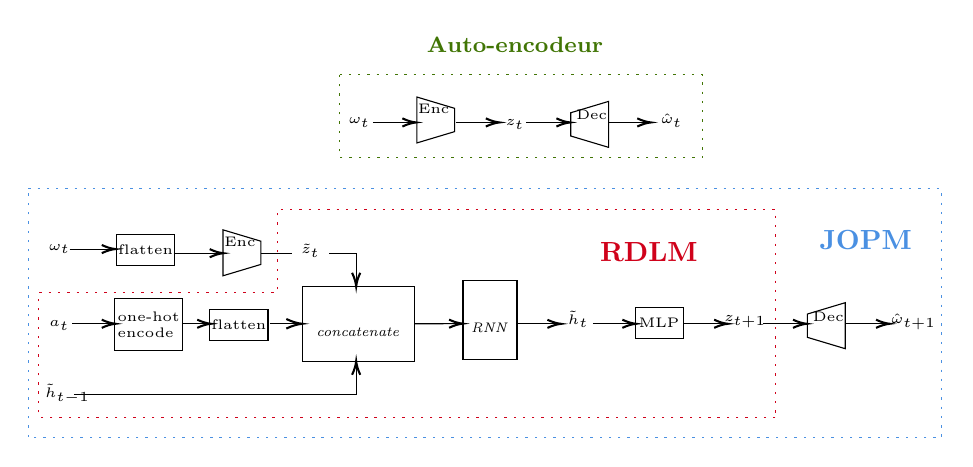
\begin{tikzpicture}[x=0.75pt,y=0.75pt,yscale=-1,xscale=1]
    %uncomment if require: \path (0,2102); %set diagram left start at 0, and has height of 2102

    %Straight Lines [id:da7905055997256106] 
    \draw    (53.06,1235.47) -- (73.06,1235.47) ;
    \draw [shift={(75.06,1235.47)}, rotate = 180] [color={rgb, 255:red, 0; green, 0; blue, 0 }  ][line width=0.75]    (6.56,-1.97) .. controls (4.17,-0.84) and (1.99,-0.18) .. (0,0) .. controls (1.99,0.18) and (4.17,0.84) .. (6.56,1.97)   ;
    %Straight Lines [id:da5451220917566785] 
    \draw    (54.23,1271.47) -- (73.06,1271.47) ;
    \draw [shift={(75.06,1271.47)}, rotate = 180] [color={rgb, 255:red, 0; green, 0; blue, 0 }  ][line width=0.75]    (6.56,-1.97) .. controls (4.17,-0.84) and (1.99,-0.18) .. (0,0) .. controls (1.99,0.18) and (4.17,0.84) .. (6.56,1.97)   ;
    %Straight Lines [id:da4433866589105997] 
    \draw    (55.06,1305.47) -- (191.06,1305.47) -- (191.06,1291.47) ;
    \draw [shift={(191.06,1289.47)}, rotate = 90] [color={rgb, 255:red, 0; green, 0; blue, 0 }  ][line width=0.75]    (6.56,-1.97) .. controls (4.17,-0.84) and (1.99,-0.18) .. (0,0) .. controls (1.99,0.18) and (4.17,0.84) .. (6.56,1.97)   ;
    %Straight Lines [id:da9772153219599438] 
    \draw    (107.06,1271.47) -- (119.06,1271.47) ;
    \draw [shift={(121.06,1271.47)}, rotate = 180] [color={rgb, 255:red, 0; green, 0; blue, 0 }  ][line width=0.75]    (6.56,-1.97) .. controls (4.17,-0.84) and (1.99,-0.18) .. (0,0) .. controls (1.99,0.18) and (4.17,0.84) .. (6.56,1.97)   ;
    %Straight Lines [id:da08798558878605356] 
    \draw    (149.44,1271.47) -- (163.06,1271.47) ;
    \draw [shift={(165.06,1271.47)}, rotate = 180] [color={rgb, 255:red, 0; green, 0; blue, 0 }  ][line width=0.75]    (7.65,-2.3) .. controls (4.86,-0.97) and (2.31,-0.21) .. (0,0) .. controls (2.31,0.21) and (4.86,0.98) .. (7.65,2.3)   ;
    %Straight Lines [id:da5508296944602415] 
    \draw    (103.06,1237.47) -- (125.06,1237.47) ;
    \draw [shift={(127.06,1237.47)}, rotate = 180] [color={rgb, 255:red, 0; green, 0; blue, 0 }  ][line width=0.75]    (6.56,-1.97) .. controls (4.17,-0.84) and (1.99,-0.18) .. (0,0) .. controls (1.99,0.18) and (4.17,0.84) .. (6.56,1.97)   ;
    %Shape: Trapezoid [id:dp14410290094148615] 
    \draw   (126.9,1226.21) -- (145.13,1231.68) -- (145.13,1242.88) -- (126.9,1248.35) -- cycle ;
    %Straight Lines [id:da384443735490001] 
    \draw    (145.06,1237.47) -- (191.06,1237.47) -- (191.06,1251.47) ;
    \draw [shift={(191.06,1253.47)}, rotate = 270] [color={rgb, 255:red, 0; green, 0; blue, 0 }  ][line width=0.75]    (6.56,-1.97) .. controls (4.17,-0.84) and (1.99,-0.18) .. (0,0) .. controls (1.99,0.18) and (4.17,0.84) .. (6.56,1.97)   ;
    %Straight Lines [id:da5196284966358902] 
    \draw    (219.06,1271.47) -- (240.39,1271.41) ;
    \draw [shift={(242.39,1271.41)}, rotate = 179.85] [color={rgb, 255:red, 0; green, 0; blue, 0 }  ][line width=0.75]    (6.56,-1.97) .. controls (4.17,-0.84) and (1.99,-0.18) .. (0,0) .. controls (1.99,0.18) and (4.17,0.84) .. (6.56,1.97)   ;
    %Straight Lines [id:da2885650017773205] 
    \draw    (268.95,1271.5) -- (287.78,1271.5) ;
    \draw [shift={(289.78,1271.5)}, rotate = 180] [color={rgb, 255:red, 0; green, 0; blue, 0 }  ][line width=0.75]    (6.56,-1.97) .. controls (4.17,-0.84) and (1.99,-0.18) .. (0,0) .. controls (1.99,0.18) and (4.17,0.84) .. (6.56,1.97)   ;
    %Straight Lines [id:da1683388835537969] 
    \draw    (305.06,1271.47) -- (323.89,1271.47) ;
    \draw [shift={(325.89,1271.47)}, rotate = 180] [color={rgb, 255:red, 0; green, 0; blue, 0 }  ][line width=0.75]    (6.56,-1.97) .. controls (4.17,-0.84) and (1.99,-0.18) .. (0,0) .. controls (1.99,0.18) and (4.17,0.84) .. (6.56,1.97)   ;
    %Straight Lines [id:da18138221495614015] 
    \draw    (349.06,1271.47) -- (356.46,1271.47) -- (368.1,1271.47) ;
    \draw [shift={(370.1,1271.47)}, rotate = 180] [color={rgb, 255:red, 0; green, 0; blue, 0 }  ][line width=0.75]    (6.56,-1.97) .. controls (4.17,-0.84) and (1.99,-0.18) .. (0,0) .. controls (1.99,0.18) and (4.17,0.84) .. (6.56,1.97)   ;
    %Shape: Trapezoid [id:dp15428640042958097] 
    \draw   (426.67,1283.47) -- (408.44,1278) -- (408.44,1266.79) -- (426.67,1261.32) -- cycle ;
    %Straight Lines [id:da8308982689158874] 
    \draw    (387.06,1271.47) -- (406.1,1271.47) ;
    \draw [shift={(408.1,1271.47)}, rotate = 180] [color={rgb, 255:red, 0; green, 0; blue, 0 }  ][line width=0.75]    (6.56,-1.97) .. controls (4.17,-0.84) and (1.99,-0.18) .. (0,0) .. controls (1.99,0.18) and (4.17,0.84) .. (6.56,1.97)   ;
    %Straight Lines [id:da854779381814783] 
    \draw    (427.06,1271.47) -- (446.1,1271.47) ;
    \draw [shift={(448.1,1271.47)}, rotate = 180] [color={rgb, 255:red, 0; green, 0; blue, 0 }  ][line width=0.75]    (6.56,-1.97) .. controls (4.17,-0.84) and (1.99,-0.18) .. (0,0) .. controls (1.99,0.18) and (4.17,0.84) .. (6.56,1.97)   ;
    %Shape: Trapezoid [id:dp12236333694521873] 
    \draw   (220.29,1162.21) -- (238.52,1167.68) -- (238.52,1178.88) -- (220.29,1184.35) -- cycle ;
    %Shape: Trapezoid [id:dp4232724503855386] 
    \draw   (312.67,1186.47) -- (294.44,1181) -- (294.44,1169.79) -- (312.67,1164.32) -- cycle ;
    %Straight Lines [id:da0811328179216142] 
    \draw    (313.06,1174.47) -- (331.06,1174.47) ;
    \draw [shift={(333.06,1174.47)}, rotate = 180] [color={rgb, 255:red, 0; green, 0; blue, 0 }  ][line width=0.75]    (6.56,-1.97) .. controls (4.17,-0.84) and (1.99,-0.18) .. (0,0) .. controls (1.99,0.18) and (4.17,0.84) .. (6.56,1.97)   ;
    %Straight Lines [id:da33212985731507805] 
    \draw    (199.06,1174.47) -- (217.89,1174.47) ;
    \draw [shift={(219.89,1174.47)}, rotate = 180] [color={rgb, 255:red, 0; green, 0; blue, 0 }  ][line width=0.75]    (6.56,-1.97) .. controls (4.17,-0.84) and (1.99,-0.18) .. (0,0) .. controls (1.99,0.18) and (4.17,0.84) .. (6.56,1.97)   ;
    %Straight Lines [id:da7950301814204398] 
    \draw    (239.06,1174.47) -- (258.1,1174.47) ;
    \draw [shift={(260.1,1174.47)}, rotate = 180] [color={rgb, 255:red, 0; green, 0; blue, 0 }  ][line width=0.75]    (6.56,-1.97) .. controls (4.17,-0.84) and (1.99,-0.18) .. (0,0) .. controls (1.99,0.18) and (4.17,0.84) .. (6.56,1.97)   ;
    %Straight Lines [id:da8317125190119203] 
    \draw    (273.06,1174.47) -- (292.1,1174.47) ;
    \draw [shift={(294.1,1174.47)}, rotate = 180] [color={rgb, 255:red, 0; green, 0; blue, 0 }  ][line width=0.75]    (6.56,-1.97) .. controls (4.17,-0.84) and (1.99,-0.18) .. (0,0) .. controls (1.99,0.18) and (4.17,0.84) .. (6.56,1.97)   ;
    %Shape: Polygon [id:ds33250073085001886] 
    \draw  [color={rgb, 255:red, 208; green, 2; blue, 27 }  ,draw opacity=1 ][dash pattern={on 0.84pt off 2.51pt}] (393.06,1316.47) -- (38.06,1316.47) -- (38.06,1256.47) -- (153.06,1256.47) -- (153.06,1216.47) -- (393.06,1216.47) -- cycle ;
    %Shape: Rectangle [id:dp3415456817493894] 
    \draw  [color={rgb, 255:red, 74; green, 144; blue, 226 }  ,draw opacity=1 ][dash pattern={on 0.84pt off 2.51pt}] (33.06,1206.47) -- (473.06,1206.47) -- (473.06,1326.47) -- (33.06,1326.47) -- cycle ;
    %Shape: Rectangle [id:dp9296059531842202] 
    \draw  [color={rgb, 255:red, 65; green, 117; blue, 5 }  ,draw opacity=1 ][dash pattern={on 0.84pt off 2.51pt}] (183.06,1151.47) -- (358.06,1151.47) -- (358.06,1191.47) -- (183.06,1191.47) -- cycle ;


    % Text Node
    \draw (332.06,1236.97) node  [color={rgb, 255:red, 208; green, 2; blue, 27 }  ,opacity=1 ] [align=left] {\textbf{RDLM}};
    % Text Node
    \draw (436.56,1230.97) node  [color={rgb, 255:red, 74; green, 144; blue, 226 }  ,opacity=1 ] [align=left] {\textbf{JOPM}};
    % Text Node
    \draw (267.56,1136.97) node  [color={rgb, 255:red, 65; green, 117; blue, 5 }  ,opacity=1 ] [align=left] {{\footnotesize \textbf{Auto-encodeur}}};
    % Text Node
    \draw (192.56,1174.47) node  [font=\tiny] [align=left] {$\displaystyle \omega _{t}$};
    % Text Node
    \draw (343.06,1173.47) node  [font=\tiny] [align=left] {$\displaystyle \hat{\omega }_{t}$};
    % Text Node
    \draw (304.56,1170.97) node   [align=left] {{\tiny Dec}};
    % Text Node
    \draw (228.44,1167.97) node   [align=left] {{\tiny Enc}};
    % Text Node
    \draw (267.56,1175.47) node  [font=\tiny] [align=left] {$\displaystyle z_{t}$};
    % Text Node
    \draw (459.6,1270.47) node  [font=\tiny] [align=left] {$\displaystyle \hat{\omega }_{t+1}$};
    % Text Node
    \draw (418.56,1267.97) node   [align=left] {{\tiny Dec}};
    % Text Node
    \draw (378.56,1270.47) node  [font=\tiny] [align=left] {$\displaystyle z_{t+1}$};
    % Text Node
    \draw (135.06,1231.97) node   [align=left] {{\tiny Enc}};
    % Text Node
    \draw (298.06,1269.47) node  [font=\tiny] [align=left] {$\displaystyle \tilde{h}_{t}$};
    % Text Node
    \draw    (242.54,1250.47) -- (268.54,1250.47) -- (268.54,1288.47) -- (242.54,1288.47) -- cycle  ;
    \draw (255.54,1269.47) node  [font=\tiny] [align=left] {\begin{minipage}[lt]{14.99pt}\setlength\topsep{0pt}
            \begin{center}
                \phantom{X}\\\textit{RNN}
            \end{center}

        \end{minipage}};
    % Text Node
    \draw  [color={rgb, 255:red, 255; green, 255; blue, 255 }  ,draw opacity=1 ][fill={rgb, 255:red, 255; green, 255; blue, 255 }  ,fill opacity=1 ]  (160.56,1227.47) -- (177.56,1227.47) -- (177.56,1245.47) -- (160.56,1245.47) -- cycle  ;
    \draw (169.06,1236.47) node  [font=\tiny] [align=left] {$\displaystyle \tilde{z}_{t}$};
    % Text Node
    \draw    (165.06,1253.47) -- (219.06,1253.47) -- (219.06,1289.47) -- (165.06,1289.47) -- cycle  ;
    \draw (192.06,1271.47) node  [font=\tiny] [align=left] {\begin{minipage}[lt]{34pt}\setlength\topsep{0pt}
            \begin{center}
                \phantom{X}\\\textit{concatenate}
            \end{center}

        \end{minipage}};
    % Text Node
    \draw    (120.56,1264.47) -- (148.56,1264.47) -- (148.56,1279.47) -- (120.56,1279.47) -- cycle  ;
    \draw (134.56,1271.97) node  [font=\tiny] [align=left] {flatten};
    % Text Node
    \draw (52.06,1305.47) node  [font=\tiny] [align=left] {$\displaystyle \tilde{h}_{t-1}$};
    % Text Node
    \draw (48.06,1272.47) node  [font=\tiny] [align=left] {$\displaystyle a_{t}$};
    % Text Node
    \draw (48.06,1235.47) node  [font=\tiny] [align=left] {$\displaystyle \omega _{t}$};
    % Text Node
    \draw    (325.56,1263.47) -- (348.56,1263.47) -- (348.56,1278.47) -- (325.56,1278.47) -- cycle  ;
    \draw (337.06,1270.97) node  [font=\tiny] [align=left] {MLP};
    % Text Node
    \draw    (74.56,1259.47) -- (107.56,1259.47) -- (107.56,1284.47) -- (74.56,1284.47) -- cycle  ;
    \draw (91.06,1271.97) node  [font=\tiny] [align=left] {one-hot\\encode};
    % Text Node
    \draw    (75.56,1228.47) -- (103.56,1228.47) -- (103.56,1243.47) -- (75.56,1243.47) -- cycle  ;
    \draw (89.56,1235.97) node  [font=\tiny] [align=left] {flatten};


\end{tikzpicture}
    }
    \caption{Schematic of the architecture of a JOPM including the RLDM and the Auto-encoder.}
    \label{fig:jopm_architecture}
\end{figure}

% \widetilde{\hat{\omega }}_{t}

More precisely, each joint observation $\omega_t^{j} = (\omega_t^1, \dots, \omega_t^{|\mathcal{A}|}) \in \Omega^{j}$ is flattened into a single vector $\tilde{\omega}_t = vec (\omega_t^1, \dots, \omega_t^{|\mathcal{A}|})$, then passed through an encoder $Enc~: \tilde{\Omega}\rightarrow Z$ to produce a latent representation $z_t = Enc(\tilde{\omega}_t)$. A decoder $Dec~: Z \rightarrow \widetilde{\hat{\Omega}}$ allows the flattened joint observation $\widetilde{\hat{\omega}}_t = Dec(z_t)$ to be reconstructed before being recomposed into an approximate joint observation $\hat{\omega}_t^{j} = unvec(\widetilde{\hat{\omega}}_t) = (\hat{\omega}_t^1, \dots, \hat{\omega}_t^{|\mathcal{A}|}) \in \Omega^ {j}$.

MLPs or attention-based architectures are generally used for the autoencoder (encoder-decoder set) in order to aggregate multi-agent information into fixed-size feature vectors while capturing critical dependencies between agents.

Once encoding has been performed on the set of joint observations $\omega^j \in \Omega^{j}$ to obtain the latent representations $z_t \in Z_t$, the multi-agent World Model operates as in a single-agent context, using the encoded observations $z_t$ in the histories transmitted to the \textbf{RLDM} $\mathcal{T}^{z}$; an \textbf{RLDM} can also be used. For each of the collected episodes $h^j \in \mathcal{D}_{H^j} $, for each step $t \in \llbracket 0, n_{step} \rrbracket$, the latent representation of the joint observation $z_t$ is concatenated with the recurrent hidden state vector $\tilde{h}_{t-1}$ and the flattened joint action vector $\tilde{a}_t$. The vector resulting from this concatenation is passed through the \textbf{RNN} (\textbf{LSTM}) to update the recurrent hidden state vector $\tilde{h}_{t}$ and then passed through an \textbf{MLP} to determine the latent representation of the approximate joint observation at the next time step $z_{t+1} $. Next, the decoder $Dec$ is used to reconstruct the flattened approximate joint observation $\tilde{\hat{\omega}}_{t+1}^{j}$. Finally, this flattened approximate joint observation is recomposed into a predicted joint observation for the next state $\hat{\omega}_ {t+1}^{j}$. In the context of \textbf{MAMAD}, \textit{World Models} are one of the core elements of the simulation implemented by the modeling activity, acting as Digital Twins of the target environment.


\subsubsection*{Description and implementation in the activity}
% Present the generic algorithm for the modeling activity (inputs → outputs).
% Include the pseudo-code/algorithm in LaTeX environment as in the previous chapter.

\autoref{alg:modeling} describes the general flow of the modeling activity.
Each step is explained below in order to clarify its objectives and role in the construction of the final model.


\begin{algorithm}[h!]
    \caption{Algorithmic view of the modeling activity.}
    \label{alg:modeling}
    \DontPrintSemicolon
    
    \KwIn{
    Initial environment $\mathcal{E}$,
    joint histories $\mathcal{D}_{H^j}$~;
    informal objective $\mathcal{G}_{\text{inf}}$~;
    discount factor $\gamma$~;
    action space $A$~;
    observation space $\Omega$
    }
    \KwOut{the simulated environment $d \in D \cup OD$}
    
    \vspace{0.5em}
    \tcp{1. Manual formalization of component functions}
    $(R^j_H, S^j_H, \texttt{Render}^j_H) \gets \texttt{manual\_formalize}(\mathcal{G}_{\text{inf}}, \mathcal{E}, A, \Omega)$ \;
    
    \vspace {0.5em}
    \If{\textit{user wants manual modeling}}{
        \Return{$(S,\{A_i\},T,R,\{\Omega_i\},O,\gamma) \gets \texttt{manual\_model}(\mathcal{G}_{\text{inf}}, \mathcal{E}, A, \Omega)$} \;
    }
    
    \vspace{0.5em}
    \tcp{2. Train autoencoders for observations}
    Extract observations $\Omega^j = \{\omega^j_t\}$ from histories $\mathcal{D}_{H^j}$ \;
    Train an autoencoder $(Enc, Dec)$ on $\Omega^j$ by minimizing the reconstruction error \;
    
    \vspace{0.5em}
    \tcp{3. Encode observations in histories}
    For each history $h^j = (\omega_t^j, a_t^j) \in \mathcal{D}_{H^j}$, encode each joint observation ${z}_t = Enc(\omega^j_t)$ to form the training set $\mathcal{B} = \{ \{(z_t, a^j_t, z_{t+1})\} = h_z^j, h_z^j \in \mathcal{D}_{H^j}\}$
    
    \vspace{0.5em}
    \tcp{4. Train the \textbf{RLDM}}
    Initialize the \textbf{RLDM} $\mathcal{T}^z = f(g)$
    
    \For{$h_z^j \in \mathcal{B}$}{
        \For{$(z_t, a^j_t, z_{t+1}) \in h^j$} {
            Train the \textbf{RLDM} $\mathcal{T}^{z}$ by minimizing the mean squared error (\textbf{MSE}) between the prediction $\hat{z}_{t+1}$ and the actual value $z_{t+1}$.
        }
    }
    
    \vspace{0.5em}
    \tcp{5. Save the initial observations and train the JOPM}
    
    $\Omega^{\mathcal{T}^j}_0 \gets \{\omega^j_0\}$ extracted from the histories $\mathcal{D}_{H^j}$
    
    $\mathcal{T}^j(h_{t-1}, \omega_t, a_t) = \langle f(h_{t-1}, Enc(\omega^j_t), a^j_t), Dec(\mathcal{T}^{z}(h_{t-1}, Enc(\omega^j_t), a^j_t)) \rangle$ \;
    
    \vspace{0.5em}
    \tcp{6. Return the modeled elements}
    \Return{$(\mathcal{T}^j, \Omega^{\mathcal{T}^j}_0, R^j_H, S^j_H, \texttt{Render}^j_H)$}
\end{algorithm}



\paragraph*{Step 1: Manual formalization of component functions.}
The first step consists of manually deriving three fundamental functions from informal descriptions of the overall objective and organizational constraints: the reward function $R^j_H$, the stop function $S^j_H$, and the optional rendering function $Render^j_H$.
This step requires the expertise of designers, who must transform high-level objectives (often expressed in natural language or in the form of business rules) into formal specifications that allow trajectories to be evaluated in the simulated environment.

\paragraph*{Step 2: Training autoencoders for observations.}
Once the interaction histories have been collected, the joint observations $\ Omega^j$ are extracted.
As their dimension can be very high in a multi-agent context, they are compressed using autoencoders.
The encoder $Enc$ learns to transform observations into compact latent representations $z_t$, while the decoder $Dec$ reconstructs the original observations from these latents.
The goal is to minimize the reconstruction error, thus ensuring that the latents retain the essential information.

\paragraph*{Step 3: Encoding observations in histories.}
The trained autoencoders are then used to transform the set of histories $\mathcal{D}_{H^j}$ into sequences of latent states.
Each observation $\omega_t^j$ is converted into a representation $z_t$, which allows a new training set $\mathcal{B}$ to be constructed, composed of triplets $(z_t, a_t^j, z_{t+1})$.
This encoding reduces the complexity of the input data and prepares the dynamic model for training.

\paragraph*{Step 4: Training the recurrent latent dynamics model (RLDM).}
A recurrent latent dynamics model (\textbf{RLDM}) is trained from the encoded set $\mathcal{B}$.
This model, denoted $\mathcal{T}^z$, learns to predict the evolution of latent states based on the hidden history $\tilde{h}_{t-1}$, the current encoded state $z_t$, and the joint action $a_t^j$.
Training is performed by minimizing the mean squared error between the prediction $\hat {z}_{t+1}$ and the actual latent $z_{t+1}$.
This learning mechanism makes it possible to capture the dynamics of the environment without direct access to the global state.

\paragraph*{Step 5: Construction of the JOPM.}
Once the \textbf{RLDM} has been trained, the initial observations $\Omega^{\mathcal {T}^j}_0$ are extracted from the histories and used to initialize the simulator.
The \textbf{JOPM} $\mathcal{T}^j$ is then defined by combining the recurrent model $f$, the encoder $Enc$, and the decoder $Dec$.
Thus, for any given observation and action, $\mathcal{T}^j$ updates the hidden state and generates a predicted observation, thereby constituting a complete simulator of multi-agent interactions.

Step 6: Activity outputs.
Finally, the activity returns all modeled elements: the \textbf{JOPM} $\mathcal{T}^j$, the set of initial observations $\Omega^{\mathcal{T}^j}_0$, the reward function $R^j_H$, the stop function $S^j_H$, and the optional rendering function $Render^j_H$.
These components constitute the core of the Digital Twin that will be used by the training, analysis, and transfer activities of the \textbf{MAMAD} method.



\subsection{Training}\label{sec:training}

The \textit{training activity} consists in optimizing the joint policies of agents in the simulated environment, taking into account organizational constraints.
It corresponds to the resolution phase of the design problem, exploiting the models produced by the modeling activity.
This activity is crucial: it leverages MARL to learn adaptive policies while using organizational abstractions to improve explainability and control.

\subsubsection*{Formal objectives}

The \textbf{inputs} of the training activity are:
\begin{itemize}
    \item the simulated environment $d \in D \cup OD$ produced by the modeling activity~;
          % \item the \textbf{JOPM} $\mathcal{T}^j$ produced by modeling;
          % \item the initial observations $\Omega^{\mathcal{T}^j}_0$;
          % \item the history-based reward function $R^j_H$
          % \item the history-based stop function $S^j_H$;
          % \item the history-based rendering function $\texttt{Render}^j_H$ or empty $\emptyset$;
    \item the organizational specifications $\mathcal{MM}$ possibly derived from the organizational specifications of a previous refinement cycle;
    \item the informal organizational specifications $\mathcal{C}_{\text{inf}}$, particularly if this is the first refinement cycle.
          % \item the discount factor $\gamma$;
          % \item the observation space $\Omega$;
          % \item the action space $A$;
\end{itemize}

\noindent
The \textbf{expected output} is a trained joint policy $\pi^j = \{\pi^j_0, \pi^j_1, \dots, \pi^j_{|\mathcal{A}|}\}$.

\medskip
\noindent

\noindent The overall relationship can be expressed as:
\begin{displaymath}
    \texttt{train}: (D \cup OD) \times \mathcal{MM} \times \mathcal{C}_{\text{inf}} \rightarrow \pi^j
\end{displaymath}

If $d \in OD$, then $d = (\Omega, A, \mathcal{T}^j, \Omega^{\mathcal{T}^j}_0, R^j_H, S^j_H, \texttt{Render}^j_H, \gamma)$, and if $d \in D$, then $d = (S,\{A_i\},T,R,\{\Omega_i\}, \allowbreak O,\gamma)$.


\subsubsection*{Positioning and proposed contribution}

Training under organizational constraints combines advances in MARL (CTDE, policy gradients, value-based methods) with constrained RL (CPO, DCQL), reward shaping and shielding. Prior work provides mechanisms for numerical/safety constraints but lacks a unified way to inject rich, symbolic organizational models (e.g., $\mathcal{M}OISE^+$) into learned multi-agent world models.

Our intended contribution is to adapt MOISE+MARL to operate directly with learned multi-agent World Models: we lift MOISE+MARL from Dec-POMDPs with access to true states to the ODec-POMDP formalism driven by a JOPM, making organizational control compatible with simulators learned from joint histories; we specify how the three constraint guides (rag, rrg, grg) apply to encode joint observations and latent dynamics by computing action masking and rewards shaping from JOPM outputs and per-agent encoded observations; and we provide a training scheme that integrates JOPM rollouts, action-masking hooks and shaped rewards into standard MARL workflows (CTDE-compatible), allowing off-the-shelf MARL algorithms to learn policies that respect organizational specifications in the learned simulator (thereby making organizationally guided MARL usable when only observable joint histories are available).


\subsubsection*{Extension of MOISE+MARL to Multi-Agent World Models}
\label{sec:multi_agent_world_models}

\noindent In realistic environments, only transitions from the history of actions and observations received are available. To better represent this context, we introduce a new formalism called \textbf{\textbf{Dec-POMDP} based on observations} (\textbf{ODec-POMDP}). An \textbf{ODec-POMDP} $d \in OD$ (where $OD$ is the set of ODec-POMDPs) is defined as a 7-tuple~:
%
$d = (\Omega, A, \mathcal{T}^j, \Omega^{\mathcal{T}^j}_0, R^j_H, S^j_H, \texttt{Render}^j_H)$
%
where~:
\begin{itemize}
    \item $\Omega$, the observation space~;
    \item $A$, the action space~;
    \item $\mathcal{T}^j$, the \textbf{JOPM} estimating the next joint observation $\omega'$ from the history $\tilde{h} \in \mathcal{H}$, the current joint observation $\omega$ and the joint action $a$. The model also returns the updated recurrent hidden state $\tilde{h}'$~;
    \item $\Omega^{\mathcal{T}^j}_0$, the set of initial joint observations;
    \item $R^j_H~: H \times \Omega \times A \times \Omega \rightarrow \mathbb{R}$, the history-based reward function, calculating the reward from the previous history, the current observation and action, and the next observation;
    \item $S^j_H~: H \rightarrow \{0,1\}$ the history-based stop function that indicates whether the agent has reached the end of its episode or achieved its goal;
    \item $\texttt{Render}^j_H : H \rightarrow \emptyset$, an optional history-based visual rendering function;
    \item $\gamma \in [0, 1]$, the discount factor.
\end{itemize}

\noindent This formulation allows \textbf{MARL} agents to operate solely on observable data, making the method compatible with learned simulated environments.

\subsubsection*{Solving an \textbf{ODec-POMDP} with MOISE+MARL}

Solving an \textbf{ODec-POMDP} with constraints $mm \in \mathcal{MM}$ consists of finding a joint policy $\pi^j = \{\pi^j_0, \pi^j_1, \dots, \pi^j_{|\mathcal{A}|}\}$ that maximizes the expected cumulative reward (or satisfies a minimum threshold), via the observation-based value function $V_{\mathcal{T}^j}^{\pi^j}$. This function represents the expected return from an initial joint observation $\omega^j \in \Omega^{\mathcal{T}^j} _0$, a history $h^j$, and a hidden state $\tilde{h}$, by applying joint actions $a^j \in A^{|\mathcal{A}|}$ under organizational constraints $\mathcal{MM}$, and using $\mathcal{T}^j$ to approximate transitions.

The complete definition of $V_{\mathcal{T}^j}^{\pi^j}$ is given in \hyperref[eq:single_value_function_parallel]{Definition 2}, and incorporates role-based (in red) and mission-based (in blue) adaptations, which influence both the joint action space and the reward. \autoref{fig:mm_synthesis} illustrates how $\mathcal{M}OISE^+$ specifications are injected into the resolution of an \textbf{ODec-POMDP} using the MOISE+MARL framework.

\medskip


\begin{figure*}[h!]
    \label{eq:single_value_function_parallel}
    \raggedright
    \textbf{\textit{Definition 2} \quad Observation-Value function adapted to constraint guides in parallel mode:}
    
    \begin{scriptsize}
        \vspace{-0.6cm}
        \begin{gather*}
            V^{\pi^j}(\tilde{h}_{t-1},h^j_{t-1},\hat{\omega}^j_t) = \hspace{-0.95cm}
            %
            \sum_{\textcolor{red}{ \substack{a^j_{t} \in A^j \text{ if } rn() < ch_{t}, \\
            a^j_{t} \in A^j_{t} \text{ else}}
            }}{\hspace{-0.9cm} \pi_i(a^j_{t} | \hat{\omega}^j_t)}
            %
            \hspace{-1.2cm}
            \sum_{\phantom{XXXX}(\tilde{h}_t,\hat{\omega}^j_{t+1}) \in \mathcal{H} \times \hat{\Omega}^j}
            %
            {\hspace{-1.2cm} \mathcal{T}^j(\langle \tilde{h}_t,\hat{\omega}^j_{t+1} \rangle | \tilde{h}_{t-1}, \hat{\omega}_t, a^j_{t})
            \Bigl[R^j_H(h^j_{t-1},\hat{\omega}^j_t,a^j_t,\hat{\omega}^j_{t+1}) \hspace{-0.1cm} }
        \end{gather*}
        %
        \vspace{-1cm}
        \begin{gather*}
            \hspace{3.6cm}
            {+ \  \textcolor{blue}{grg^j_m(h^j_t)}
            +
            \textcolor{red}{(1-ch_t) \times rrg^j(h^j_{t-1},\hat{\omega}^j_t,a^j_{t+1})} + V^{\pi^j}(\tilde{h}_{t}, h^j_t, \hat{\omega}^j_{t+1})\Bigr]}
        \end{gather*}
        %
        \vspace{-0.15cm}
        %
        \[\hspace{-0.9cm}\text{With \ } \tilde{h}_{-1} = \mathbf{0} \text{ and } \tilde{\omega}^j_0 \in \Omega_0^{\mathcal{T}^j} \text{ ; } a^j_t = \langle a_{t,0}, a_{t,1} \dots a_{t,|\mathcal{A}|} \rangle \text{ ; } \omega^j_t = \langle \omega_{t,0}, \omega_{t,1} \dots \omega_{t,|\mathcal{A}|} \rangle \text{ ; }\]
        %
        \vspace{-0.25cm}
        \[\hspace{-5.85cm} h^j_t = \langle h_{t,0}, h_{t,1} \dots h_{t,|\mathcal{A}|} \rangle = \langle \langle h_{t-1,i}, \omega_{t,i}, a_{t,i} \rangle \rangle_{i \in \mathcal{A}}\]
        %
        \vspace{-0.2cm}
        \textcolor{red}{\[\hspace{-2.6cm}\text{ \hspace{-0.1cm} With } \langle rag_i, rrg_i \rangle = rcg(ar(i)) \text{ ; } rn: \emptyset \to [0,1[ \text{, a uniform random function}\]}
        %
        \vspace{-0.3cm}
        \textcolor{red}{\[A^j_t \times \mathbf{R}^{|\mathcal{A}|} \hspace{-0.1cm} = \hspace{-0.1cm} rag^j(h^j_t, \tilde{\omega}^j_t) \hspace{-0.1cm} = \hspace{-0.1cm} \langle rag_i(h_{t,i}, \omega_{t,i}) \rangle_{i \in \mathcal{A}} \text{ ; } rrg^j(h^j_{t-1}, \tilde{\omega}^j_t, a^j_t) \hspace{-0.1cm} = \hspace{-0.1cm} \sum_{i \in \mathcal{A}}{rrg_i(h_{t-1,i}, \omega_{t,i}, a_{t,i})}\]}
        %
        \vspace{-0.75cm}
        \textcolor{blue}{
            \begin{gather*}
                \hspace{-1.7cm} grg_m(h) = \hspace{-1cm} \sum_{\hspace{0.3cm}(grg_i,w_i) \in mo(m)}{\hspace{-1.1cm} w_i \times grg_i(h)}
                \text{ ; }
                grg^j_m(h^j_t) = \hspace{-0.1cm} \sum_{i \in \mathcal{A}}{\sum_{m \in \mathcal{M}_i}{ \hspace{-0.1cm} v_m(t) \frac{grg_m(h_{t,i})}{1 - p + \epsilon} }} \text{ ; } \epsilon \in \mathbb{R}_{>0} \text{ ; }
            \end{gather*}
        }
        \vspace{-0.9cm}
        \textcolor{blue}{
            \begin{gather*}
                \hspace{-4cm}
                v_m(t) = \{ 1 \text{ if } t \in t_c \text{ ; else } 0 \} \text{ ; } \mathcal{M}_i = \{m_j | \langle ar(i),m_j,t_c,p \rangle \in \mathcal{M}\}
            \end{gather*}
        }
    \end{scriptsize}
    
\end{figure*}


\noindent In parallel mode, at each time step $t \in \mathbb{N}$ (starting at $t=0$), each agent $i \in \mathcal{A}$ is assigned a role $\rho_i = ar (i)$. For each temporally valid deontic specification $d_i = rds(\rho_i) = \langle tc_i, y_i, m_i \rangle$, the agent is either authorized ($y_i = 0$) or obligated ($y_i = 1$) to engage in mission $m_i \ in \mathcal{M}$, with set of objectives $\mathcal{G}_{m_i} = mo(m_i)$.

When agents observe $\tilde{\omega}_t^j$, they select their actions from $A_{i,t}$ (derived via role reward guides) with probability $ch_t$, or in $A_t$ otherwise. If $ch_t = 1$, agents are strictly constrained by their role.

Observation and state transitions are approximated via \textbf{JOPM} $\mathcal{T}^j$ from the previous hidden state $\tilde{h}_{t-1}$, the joint observation $\omega^j_t$, and the joint action $a^j_t$. The reward function $R^j_H$ uses this same information, along with the next observation, to produce the reward. Bonuses or penalties are then added according to:
i) the achievement of valid objectives (via the objective reward guides, weighted by $\frac{1}{1 - p + \epsilon}$),
ii) role compliance (via the role reward guides, weighted by $1 - ch_t$).

Although not indicated, in practice the stop function $S^j_H$ is used instead of the discount factor to terminate the step loop. Most often, this stop function consists of returning true when a threshold number of steps has been reached.
%
Similarly, if the history-based rendering function $\texttt{Render}$ is provided, it is used to visualize each agent's observations. This function is used primarily for explainability and supervision purposes.


\subsubsection*{Description and implementation in the activity}

\autoref{alg:training_mamad} describes the general course of the training activity.
Each step is detailed below.

\paragraph*{Step 1: Formalization of constraints.}
If the specifications $\mathcal{MM}$ are not provided, they are derived manually from the informal constraints $\mathcal{C}_{\text{inf}}$.

\paragraph*{Step 2: Initialization.}
Initialize the parameters of the joint policy $\pi^j$ and an experience buffer $\mathcal{B}$.

\paragraph*{Step 3: Execute simulated episodes.}
For each episode, sample an initial observation $\omega_0^j \in \Omega^{\mathcal{T}^j}_0$, initialize the history $h_{-1}^j$ and the hidden state $\tilde{h}_{-1}$.

\paragraph*{Step 4: Select actions under constraints.}
At each step $t$, calculate the set of allowed actions $A_t^j = rag^j(h^j_t,\omega_t^j)$.
The agent selects its action $a_t^j$ from $A_t^j$ with probability $ch_t$, otherwise from $A$.

\paragraph*{Step 5: Transition and update of the JOPM.}
The transition $(\tilde{h}_t,\omega_{t+1}^j)$ is generated by $\mathcal{T}^j(\tilde{h}_{t-1},\omega_t^j,a_t^j)$.

\paragraph*{Step 6: Calculation of rewards.}
The reward $r_t$ combines:
\begin{itemize}
    \item the base reward $R^j_H$,
    \item a bonus $grg^j(h^j_t)$ if objectives are achieved,
    \item a bonus/penalty $(1-ch_t)\times rrg^j(h^j_t,\omega_t^j,a_t^j)$ related to role compliance.
\end{itemize}

\paragraph*{Step 7: Experience update and learning.}
Transitions are stored in $\mathcal{B}$, and the policy $\pi^j$ is optimized by any compatible \textbf{MARL} algorithm (Q-learning, Policy Gradient, \textbf{CTDE}, etc.).

\paragraph*{Step 8: Output.}
At the end of the episodes, the activity returns the trained joint policy $\pi^j$.


\begin{algorithm}[h!]
    \caption{Algorithmic view of the training activity.}
    \label{alg:training_mamad}
    \DontPrintSemicolon
    
    \KwIn{
    Simulated environment as \textbf{Dec-POMDP} or \textbf{ODec-POMDP} $d \in D \cup OD$~;
    Organizational specifications $\mathcal{MM}$;
    Informal design constraints $\mathcal{C}_{\text{inf}}$;
    }
    \KwOut{$\pi^j$: Trained joint policy}
    
    \vspace{0.3em}
    
    \If{$\mathcal{MM} = \emptyset$}{
        $\mathcal{MM} \gets \texttt{manual\_formalize}(\mathcal{C}_{\text{inf}})$ \tcp*{Manual formalization of org. specs.} \;
    }
    
    \tcp*[l]{If env. simulated manually, classical training}
    \If{$d \in D$}{
        \textit{train a joint policy $\pi^j$ via constrained MARL according to \hyperref[eq:single_value_function]{Definition 1}} \;
    }
    \Else{
    
    Initialize policy parameters $\pi^j$ and replay buffer $\mathcal{B}$ \;
    
    \ForEach{episode $e = 1 \dots N$}{
    Sample $\omega_0^j \sim \Omega_0^{\mathcal{T}^j}$, initialize $\tilde{h}_{-1} \gets \mathbf{0}$ \;
    Initialize history $h_{-1}^j \gets \emptyset$ \;
    
    \ForEach{step $t = 0 \dots T$}{
    Compute $A_t^j = rag^j(h^j_t, \omega^j_t)$ via role reward guides in $\mathcal{MM}$ \;
    \If{$rn() < ch_t$}{
        Select $a_t^j \sim \pi^j(\cdot | \omega_t^j)$ from the set $A_t^j$ (constrained) \;
    }
    \Else{
        Select $a_t^j \sim \pi^j(\cdot | \omega_t^j)$ from the set $A_t$ \;
    }
    
    $(\tilde{h}_t, \omega_{t+1}^j) \gets \mathcal{T}^j(\tilde{h}_{t-1}, \omega_t^j, a_t^j)$ \tcp*{JOPM prediction}
    
    $r_t \gets \gamma^t \times R_H^j(h^j_{t-1}, \omega_t^j, a_t^j, \omega_{t+1}^j)$ \tcp*{Base reward}
    
    $r_t \gets r_t + grg^j(h^j_t)$ \tcp*{Bonus via objective guides}
    
    $r_t \gets r_t + (1 - ch_t) \times rrg^j(h^j_t, \omega_t^j, a_t^j)$ \tcp* {Bonus/penalty via role guides}
    
    Add $(\omega_t^j, a_t^j, r_t, \omega_{t+1}^j)$ to $\mathcal{B}$ \;
    Update $h^j_t \gets \langle \langle h_{t-1,i}, \omega_{t,i}, a_{t,i} \rangle \rangle_{i \in \mathcal{A}}$ \;
    
    Train $\pi^j$ with mini-batches drawn from $\mathcal{B}$ using any \textbf{MARL} method \;
    }
    }
    }
    
    \Return{$\pi^j$}
\end{algorithm}



\subsection{Analyzing}\label{sec:analyzing}


The \textit{analysis activity}\index{Analysis (ANL)} aims to evaluate and explain the joint policies learned. It provides an explanation of the behaviors observed in terms of roles, objectives, and missions. This activity plays a central role in explainability by linking the dynamics learned to interpretable organizational structures.


\subsubsection*{Formal objectives}


The \textbf{inputs} to the analysis activity are:
\begin{itemize}
    \item an \textbf{ODec-POMDP} $d$ representing the learned simulated environment;
    \item a trained joint policy $\pi^j$;
    \item an initial organizational specification $\mathcal{MM}$ (optional);
    \item the test episode window $w_{\text{episodes}}$.
\end{itemize}

\noindent
The \textbf{expected outputs} are:
\begin{itemize}
    \item the set of inferred implicit specifications $\mathcal{MM}_{\text{inferred}}$;
    \item the organizational fit score $\texttt{org\_fit}$ on the last $w_{\text{episodes}}$ episodes;
    \item the average rewards $\overline{r}$ over the last $w_{\text{episodes}}$ episodes;
    \item the standard deviation of rewards $\sigma$ over the last $w_{\text{episodes}}$ episodes;
    \item the Boolean indicating whether the user wishes to continue the refinement cycles $\texttt{running\_refinement}$.
\end{itemize}

\noindent The overall relationship can be expressed as:
\[
    (\mathcal{MM}_{\text{inferred}}, \texttt{org\_fit}, \overline{r}, \sigma, \texttt{running\_refinement}) \gets \texttt{analyze}(d, \pi^j, \mathcal{MM}, w_{\text{episodes}})
\]


\subsubsection*{Positioning and proposed contributions}

The analysis builds on the TEMM method, which clusters trajectories to infer roles and goals and quantifies alignment via an organizational fit score. In brief: observation trajectories are clustered (distance metrics such as LCS/DTW) to extract candidate goals; state-action transition trajectories are clustered to extract candidate roles and representative transition rules; a per-item representativeness score (inverse normalized variance) selects robust representatives. Structural Organizational Fit (SOF) is computed from role-cluster variances, Functional Organizational Fit (FOF) from goal-cluster variances, and the final Organizational Fit is simply the average of these two values.

TEMM is effective but requires manual hyperparameter tuning (distance metric, cluster cutoff, representativeness threshold), which limits automation and reproducibility. Our intended contribution is to extend TEMM by automating hyperparameter selection and representativeness choice. This includes:
\begin{enumerate}
    \item Automatically search for clustering settings that produce clear and meaningful groups of trajectories, favoring compact and coherent clusters.
    \item Explore different choices for how representative a trajectory must be to be used as an example, and pick a value that balances simplicity of the specification with its usefulness for guiding learning.
    \item Apply the selected clustering and representativeness choices to extract the inferred organizational elements (roles, goals, and simple rules).
    \item Compute summary scores that quantify structural and functional alignment, and return the inferred organizational specification and an overall fit score.
\end{enumerate}



\subsubsection*{Extended TEMM method with HPO}

A major problem encountered with \textbf{TEMM} is the need to manually choose several hyperparameters (distance metrics, clustering thresholds, representativeness thresholds), which slows down the analysis process and limits its automation. Too low representativeness leads to overfitting, while too high representativeness limits constraints and slows down convergence.


To overcome this difficulty, we propose a process of ‘hyperparameter optimization’ (HPO) consisting of a grid search on possible combinations, aiming to maximize organizational fit and minimize the number of clusters:

\begin {itemize}
\item (i) For observations and transitions, apply a joint search on distance metrics and clustering thresholds to minimize intra-cluster variance and the number of clusters~;
\item (ii) Determine the minimum representativeness (structural and functional) to obtain concise and relevant objectives and roles. Decreasing this representativeness increases coverage but reduces the robustness of organizational constraints. A high value limits generalization, while too low a value leads to overfitting. This is illustrated in \autoref{fig:conv_time_repr}, where normalized convergence time is plotted against minimum representativeness. Fast convergence indicates strong and consistent organizational constraints, while slow convergence suggests weak or inconsistent constraints.
\end{itemize}

We adopt a compromise based on the \textbf{inflection point} of the convergence/time graph (see \autoref{fig:conv_time_repr}), choosing the highest representativeness that ensures a normalized convergence of 3.5%. This strategy yields useful, interpretable, and generalizable specifications without excessive complexity.

\begin{figure}[h!]
    \centering
    \includegraphics[trim=0cm 0cm 0cm 0cm, clip, width=1.\linewidth]{figures/convergence_time_relative_to_representativeness.pdf}
    \caption{Normalized convergence time as a function of minimum representativeness.}
    \label {fig:conv_time_repr}
\end{figure}


\subsubsection*{Description and implementation in the activity}

The \autoref{alg:auto_temm} formalizes the general course of the analysis activity.
Each step is detailed below in order to explain the mechanisms that allow us to infer an implicit organizational specification and calculate organizational adequacy.


\begin{algorithm}[h!]
    \caption{Algorithmic view of the analysis activity (Auto-TEMM)}
    \label{alg:auto_temm}
    \DontPrintSemicolon
    
    \KwIn{
        Joint policy $\pi^j$~;
        \textbf{ODec-POMDP} $d$~;
        Initial specification $\mathcal{MM}$~;
        Normalized convergence threshold (default~: 3.5\%) $\eta$
    }
    
    \KwOut {
    Inferred organizational specification $\mathcal{MM}_{\text{inferred}}$;
    Organizational adequacy score $\textbf{OF}$
    }
    
    \tcp*[l]{1. Trajectory collection}
    Generate individual histories $\mathcal{D}_{\text{trans}}$ from $d$ under $\pi^j$ \;
    $\mathcal{D}_{\text{obs}} \gets$ individual observation trajectories from $\mathcal{D}_{\text{full}}$ \;
    
    \tcp*[l]{2. \textbf{HPO} on distance and clustering threshold}
    \For{$t \in \{obs, trans\}$}{
        \ForEach{distance metric $\delta_t$}{
            \ForEach{minimum cluster threshold $\tau_t$}{
                Apply clustering with $(\delta_t, \tau_t)$ \;
                Calculate $\sigma_{\text{obs}}, \sigma_{\text{trans} }, N_{\text{clusters}}$ \;
                Score $\gets \alpha (\sigma_{\text{obs}} + \sigma_{\text{trans}}) + \beta N_{\text{clusters}}$ \tcp*[l]{default~: $\alpha=0.4$, $\beta=0.6$}
                Retain $(\delta_t^*, \tau_t^*)$ with minimum Score \;
            }
        }
    }
    
    \tcp*[l]{3. Application of clustering with optimal \textbf{HPO}}
    Clustering of observations: $\mathcal{D}_{\text{obs}} \rightarrow C_{obs}$ via $(\delta_{obs}^*, \tau_{obs}^*)$ \;
    Clustering transitions: $\mathcal{D}_{\text{trans}} \rightarrow C_{trans}$ via $(\delta_{trans}^*, \tau_{trans}^*)$ \;
    
    \tcp*[l]{4. \textbf{HPO} on representativeness (convergence)}
    \For{$t \in \{obs, trans\}$}{
    \ForEach {representativeness $\rho_t$}{
    Infer $\mathcal{MM}_{\rho_t}$ from the clusters \;
    Initialize a policy $\pi^j_{\rho_t}$ \;
    Train $\pi^j_{\rho_t}$ on $(d, \mathcal{MM}_{\rho_t})$ until $R_{\min}$ is reached \;
    Record convergence time $c_{\rho_t}$ such that $ct_t(\rho_t) = c_{\rho_t}$ \;
    }
    
    \tcp*[l]{Select inflection point}
    $\rho_t^* \gets max(\{\rho_t \ | \ ct_t(\rho_t) < \eta \})$ \tcp*[r]{default $\eta = 3.5\%$}
    }
    
    \tcp*[l]{5. Inference of roles and objectives}
    Infer roles from $\mathcal{D}_{\text{trans}}, \delta^*, \tau^*, \rho^*$ \;
    Infer objectives from $\mathcal{D}_{\text{obs}}, \delta^*, \tau^*, \rho^*$ \;
    
    \tcp*[l] {6. Calculation of organizational fit}
    Calculate \textbf{SOF} and \textbf{FOF} from intra-cluster variances \;
    $\text{OF} \gets \frac{1}{2}(\text{SOF} + \text{FOF})$ \;
    
    \tcp*[l]{6.5. Manual refinement (optional)}
    $(\mathcal{MM}_{\text{inferred}} \times {0,1}) \gets \texttt{manual\_refine}(\mathcal{MM}_{\text{inferred}})$
    
    \Return{$\mathcal{MM}_{\text{inferred}}, \texttt{org\_fit}, \overline{r}, \sigma, \texttt{running\_refinement}$}
\end{algorithm}



\paragraph*{Step 1: Collect trajectories.}
The first step is to execute the joint policy $\pi^j$ in the environment $d$ in order to generate complete histories of transitions $(\omega, a, \omega')$ on the $w_{\text{episodes}}$ of the validation window. This allows us to calculate the mean $\overline{r}$ and standard deviation $\sigma$ of the rewards over the collected episodes.
In addition, two datasets are extracted from these episodes:
\begin{itemize}
    \item $\mathcal{D}_{\text{trans}}$ containing the transition sequences $(\omega_t, a_t, \omega_{t+1})$, used for role inference;
    \item $\mathcal{D}_{\text{obs}}$ containing only the observation sequences $(\omega_t)$, used for objective and mission inference.
\end{itemize}

\paragraph*{Step 2: Optimization of distances and clustering thresholds.}
To reduce variability between trajectories and identify recurring structures, the sets $\mathcal{D}_{\text{obs}}$ and $\mathcal{D}_{\text{trans}}$ are subjected to a clustering process.
Several distance metrics $\delta_t$ (e.g. \textbf{LCS}, Smith-Waterman, vector distances) and clustering thresholds $\tau_t$.
Each combination $(\delta_t, \tau_t)$ is evaluated according to a weighted score:
\[
    \text{Score} = \alpha (\sigma_{\text{obs}} + \sigma_{\text{trans}}) + \beta N_{\text{clusters}}
\]
where $\sigma$ denotes the intra-cluster variance and $N_{\text{clusters}}$ the total number of clusters.
The combination that minimizes this score is selected, ensuring a compromise between internal consistency and cluster compactness.

\paragraph*{Step 3: Application of optimal clustering.}
Once the optimal hyperparameters $(\delta^*, \tau^*)$ have been determined, the trajectories are grouped together:
\begin{itemize}
    \item the transition clusters $C_{trans}$ are used to infer \textbf{roles} by extracting common sequences (\textbf{CLS}) and associated behavioral rules;
    \item observation clusters $C_{obs}$ are used to identify \textbf{intermediate objectives} and associated plans.
\end{itemize}

\paragraph*{Step 4: Search for optimal representativeness.}
The degree of representativeness $\rho_t$ sets the minimum threshold for a transition or observation to be retained as a characteristic of a role or objective.
A grid search is performed on different values of $\rho_t$.
For each $\rho_t$, a specification $\mathcal{MM}_{\rho_t}$ is inferred, then a new policy $\pi^j_{\rho_t}$ is retrained in $d$.
The convergence time $c_{\rho_t}$ to reach a minimum performance $R_{\min}$ is then recorded.
The optimal parameter $\rho_t^*$ is chosen as the highest representativeness guaranteeing convergence below the threshold $\eta$ (default 3.5%).

\paragraph*{Step 5: Inference of roles and objectives. }
With $(\delta^*, \tau^*, \rho^*)$, we extract the roles $\mathcal{R}$, the intermediate objectives $\mathcal{G}$ and their hierarchical relationships (missions, role inheritance).
Permissions and obligations are deduced by observing the systematicity (obligations) or variability (permissions) of role-mission associations in the trajectories.

\paragraph*{Step 6: Calculation of organizational fit.}
As with \textbf{TEMM}, two partial indicators are calculated:
\begin{itemize}
    \item \textbf{\textbf{SOF}} (structural organizational fit), measuring role consistency via the variance of intra-cluster transitions;
    \item the \textbf{\textbf{FOF}} (functional organizational fit), measuring functional consistency in the achievement of intermediate objectives.
\end{itemize}
The overall indicator is obtained by aggregation:
$\text{OF} = \frac{1}{2}(\text{SOF} + \text{FOF})$

\paragraph*{Step 6.5: Understanding and refining specifications.}
At this stage, the implicit organizational specifications $\mathcal{MM}_{\text{inferred}}$ are presented in the form of constraint guides, which are similar to rules linking observations to actions (RAG) or sets of observations (GRG). If desired, the user can examine and interpret these constraint guides in order to propose new organizational specifications that are more explicit and understandable. This step is optional, but it improves the robustness and interpretability of the organizational specifications. If the user does not modify the inferred specifications, they are retained and reused in the next refinement cycle to restrict the search space. If the user considers the results satisfactory, they can end the refinement cycles by setting the Boolean \texttt{running\_refinement} to 0.

We include this optional step in the relation $\text{manual\_refine}: \mathcal{MM}_{\text{inferred}} \rightarrow \mathcal{MM}_{\text{explicit}} \times {0,1}$, which takes the implicit specifications as input and returns explicit specifications (or the same ones if the user does not wish to modify them) as well as a Boolean indicating whether they wish to continue the refinement cycles.

\paragraph*{Step 7: Activity outputs.}
The activity returns:
\begin{itemize}
    \item an implicit specification $\mathcal{MM}_{\text{inferred}}$ describing automatically inferred roles, missions, permissions, and obligations;
    \item the organizational fit score $\texttt{org\_fit}$ used to quantify the organizational quality of emerging behaviors;
    \item the mean $\overline{r}$ and standard deviation $\sigma$ of rewards over the analyzed episodes;
    \item a boolean $\texttt{running\_refinement}$ indicating whether the user wishes to continue the refinement cycles.
\end{itemize}


\subsection{Transferring}\label{sec:transferring}

The \textit{transfer activity}\index{Transfer (TRF)} corresponds to the implementation and monitoring of joint policies in the real environment.
It plays a dual role: (i) ensuring the continuous execution of the most recent policy $\pi^j_{\text{latest}}$ in $\mathcal{E}$, guaranteeing the effective action of agents, and (ii) collecting new real trajectories $(\omega^j_t, a^j_t, \omega^j_{t+1})$ to enrich the database $\mathcal{D}_{H^j}$, enabling the updated simulated model and organizational specifications.

\subsubsection*{Formal objectives}

The \textbf{inputs} to the transfer activity are:
\begin{itemize}
    \item the most recent joint policy $\pi^j_{\text{latest}}$;
    \item the real environment $\mathcal{E}$;
    \item the accumulated trajectory database $\mathcal{D}_{H^j}$.
\end{itemize}

\noindent
The \textbf{expected outputs} are:
\begin{itemize}
    \item an enriched trajectory database $\mathcal{D}_{H^j}$;
    \item a $\texttt{need\_update}$ signal triggering the resumption of the design cycle.
\end{itemize}

The overall relationship can be expressed as:
\[
    (\mathcal{D}_{H^j}, \texttt{need\_update}) \gets \texttt{transfer}(\pi^j_{\text{latest}}, \mathcal{E}, \mathcal{D}_{H^j}, \texttt{mode})
\]

\subsubsection*{Positioning and proposed contributions}

Transfer and supervision in deployments combine policy transfer, domain adaptation (Sim2Real), online model calibration and continuous monitoring. Existing methods (robust RL~\cite{pinto2017robust}, domain randomization~\cite{tobin2017domain,ganin2016domain}, dynamic calibration~\cite{deisenroth2011pilco}) partially reduce sim2real gaps but rarely provide joint, online updates of both the simulator and multi-agent policies.

Main obstacles:
\begin{itemize}
    \item No unified framework to update the Digital Twin and deployed policies together;
    \item Difficulty in automatically detecting and correcting sim2real discrepancies;
    \item Limited mechanisms for safe, continuous supervision and adaptation.
\end{itemize}

We propose an asynchronous, event-driven transfer framework:
\begin{itemize}
    \item \textbf{Transfer Loop}: continuous policy execution and trajectory buffering ($\mathcal{B}$) in the field;
    \item \textbf{Update Trigger}: when $\lvert\mathcal{B}\rvert \ge \texttt{batch\_size}$, flush to $\mathcal{D}_{H^j}$ and asynchronously launch modeling/training to close the loop.
\end{itemize}

\subsubsection*{Description and implementation of the activity}

\autoref{alg:transferring} formalizes the operation of the transfer activity.
Each element is described below to clarify the mechanisms and their role in the design loop.


\vspace{-0.3em}
\begin{algorithm}[h!]
    \caption{Algorithmic view of the transfer activity.}
    \label{alg:transferring}
    \DontPrintSemicolon
    \KwIn{
    Current policy $\pi^j_{\text{latest}}$,
    real environment $\mathcal{E}$,
    trajectory base $\mathcal{D}_{H^j}$,
    transfer mode $\texttt{mode} \in \{\texttt{DIRECT}, \texttt{REMOTE}\}$
    }
    \KwOut{Updated trajectory database $\mathcal{D}_{H^j}$, update signal $\texttt{need\_update}$}
    
    \vspace{0.3em}
    \SetKwProg{Transfer}{Procedure \normalfont TransferLoop}{}{}
    \Transfer{}{
    
    \While{the \textbf{MAS} is active in the environment $\mathcal{E}$}{
    
    \uIf{$\texttt{mode} = \texttt{DIRECT}$}{
    \tcp*[l]{Each agent applies the policy locally}
    Agents observe locally $\omega^j_t$\;
    Local calculation $a^j_t \gets \pi^j_{\text{latest}}(\omega^j_t)$\;
    Local application of actions and update of state $\omega^j_{t+1}$\;
    Local storage $(\omega^j_t, a^j_t, \omega^j_{t+1})$ in an internal buffer\;
    Periodically: send local buffers to CybMASDE to update $\mathcal{D}_{H^j}$\;
    }
    \uElseIf{$\texttt{mode} = \texttt{REMOTE}$}{
    \tcp*[l]{The policy is executed by the Transferring process}
    $\omega^j_t \gets \texttt{observe}(\mathcal{E})$\;
    $a^j_t \gets \pi^j_{\text{latest}}(\omega^j_t)$\;
    $\omega^j_{t+1} \gets \texttt{apply}(\mathcal{E}, a^j_t)$\;
    Add $(\omega^j_t, a^j_t, \omega^j_{t+1})$ to temporary buffer $\mathcal{B}$\;
    }
    
    \tcp*[l]{Check if update is triggered}
    \If{$|\mathcal{B}| \geq \texttt{batch\_size}$} {
        Add $\mathcal{B}$ to $\mathcal{D}_{H^j}$ and empty $\mathcal{B}$ \;
        $\texttt{need\_update} \gets \texttt{True}$ \;
        \If{$\texttt{not running\_update} = \texttt{False}$}{
            \texttt{launch\_update()} \tcp*[r]{Asynchronous call to the MTA process}
        }
    }
    
    }
    
    }
\end{algorithm}


\paragraph*{Inputs and outputs.}
The activity receives the following inputs:
\begin{itemize}
    \item the most recent joint policy $\pi^j_{\text{latest}}$, produced during training;
    \item the real environment $\mathcal{E}$, representing the operational domain where the \textbf{MAS} acts;
    \item the current trajectory database $\mathcal{D}_{H^j}$, enriched over the course of deployments.
\end{itemize}
At the output, it returns:
\begin{itemize}
    \item an updated trajectory base $\mathcal{D}_{H^j}$;
    \item a Boolean signal $\texttt{need\_update}$ indicating whether modeling and training activities should be restarted.
\end{itemize}

\paragraph*{Transfer loop.}
The transfer loop runs as long as the \textbf{MAS} is active in $\mathcal{E}$.
At each time step $t$:
\begin{enumerate}
    \item an observation $\omega^j_t$ is collected via the function $\texttt{observe}(\mathcal{E})$;
    \item the action $a^j_t$ is chosen by applying the policy $\pi^j_{\text{latest}}$ to the current observation;
    \item this action is executed in the environment via $\texttt{apply}(\mathcal{E}, a^j_t)$, producing the new observation $\omega^j_{t+1}$;
    \item the transition $(\omega^j_t, a^j_t, \omega^j_{t+1})$ is stored in a temporary buffer $\mathcal{B}$.
\end{enumerate}

\paragraph*{Update trigger.}
When the size of the buffer $\mathcal{B}$ exceeds a threshold $\texttt{batch\_size}$, the content is added to the trajectory database $\mathcal{D}_{H^j}$ and then the buffer is emptied.
The $\texttt{need\_update}$ signal is then activated.
If no update process is in progress (\texttt{not running\_update}), the \texttt{launch\_update()} procedure is triggered asynchronously to restart the modeling and training activities.

\paragraph*{Overall operation.}
This scheme ensures three essential properties:
\begin{itemize}
    \item \textbf{continuity of execution}: agents always operate with the latest available policy;
    \item \textbf{responsiveness}: real data is integrated as soon as a sufficient volume is collected;
    \item \textbf{automation}: updates are triggered without human intervention, while avoiding conflicts between parallel processes.
\end{itemize}

\paragraph*{Formal elements.}
%
\begin{itemize}
\item $\mathcal{B}$ denotes the temporary buffer (see \autoref{alg:transferring}),
\item $\texttt{batch\_size}$ sets the granularity for triggering updates,
\item $\texttt{launch\_update}()$ ensures synchronization with the other activities of the method.
\end {itemize}



\section{Experimental setup}
\label{sec:experimental_setup}

We developed a tool that we propose to facilitate the implementation of the MAMAD method through four environments following a proposed evaluation protocol.

\subsection{CybMASDE: A development environment to implement the MAMAD method}
\label{sec:cybmasde}

To support the implementation of the MAMAD method in a reproducible and modular way, 
we developed the \textbf{Cyber Multi-Agent System Development Environment (CybMASDE)}%
\footnotemark[1], a Python-based platform designed to orchestrate the four activities of 
MAMAD---\emph{modeling}, \emph{training}, \emph{analysis}, and \emph{transfer}---under the 
MOISE+MARL framework. CybMASDE exposes three complementary user interfaces: 
(i) a command-line interface (CLI) for scripted workflows; 
(ii) a Python library for experiment definition and integration with external simulators; and 
(iii) a web-based GUI (Angular) for interactive project creation, inspection, and monitoring.

\footnotetext[1]{Source code and documentation available at
    \url{https://github.com/julien6/CybMASDE} and \url{https://julien6.github.io/CybMASDE/}.}

CybMASDE integrates natively with the Ray/RLlib ecosystem, enabling training with either 
\textbf{TensorFlow} or \textbf{PyTorch} backends through MARLlib~\cite{hu2022marllib}. 
Organizational constraints derived from MOISE+MARL are injected into the RL workflow 
through action masking hooks and reward-shaping components, ensuring policy updates 
remain consistent with the prescribed roles, missions, and norms.

\paragraph*{Modeling.}
The modeling module constructs a \emph{Joint Observation Prediction Model} (JOPM) using LSTM 
dynamics trained on joint histories $\mathcal{D}_{H^j}$. Observations are compressed using VAE 
encoders (latent size 16--64), while actions are embedded using MLPs. The LSTM 
(hidden size 64 or~128) is optimized using Adam with learning rates 
$\text{lr} \in [10^{-4}, 5 \cdot 10^{-4}]$.  
Rewards $R_H^j$ are manually formalized from informal goals $\mathcal{G}_{\text{inf}}$, while 
constraints $\mathcal{C}_{\text{inf}}$ are mapped into MOISE+MARL symbolic specifications 
$\mathcal{MM}$ via the implementation of MOISE+MARL called \textbf{MOISE+MARL API} (MMA)~\cite{soule2025moisemarl}.

\paragraph*{Training.}
CybMASDE uses MARLlib implementations (e.g., MAPPO, MADDPG), executed through RLlib. 
Training configurations include learning rates $\text{lr}\in[10^{-4}, 5\cdot 10^{-4}]$, discount 
factors $\gamma\in[0.9, 0.99]$, \textbf{Proximal Policy Optimization} clipping parameters in $[0.1, 0.3]$, batch sizes 
$\{64,128\}$, and policy networks composed of MLPs with 64--256 hidden units.

\paragraph*{Analysis.}
Auto-TEMM extends the original TEMM by incorporating full hyperparameter optimization using 
Optuna~\cite{akiba2019optuna}. Hierarchical clustering relies on distance metrics such as DTW and LCS, with cluster weights optimized to minimize intra-cluster variance and the resulting number of clusters. 
Representativeness sweeps in $[0,1]$ identify values minimizing convergence time (threshold 
3.5\%). Organizational fit aggregates SOF and FOF metrics computed from cluster statistics.

\paragraph*{Transfer and Iterative Refinement.}
Learned policies $\pi_{\text{latest}}^j$ are deployed via PettingZoo or environment-specific 
APIs. Once the trajectory buffer reaches a user-defined threshold (e.g., 512 steps), a new 
modeling--training--analysis cycle is triggered automatically. This forms the basis of the 
automated MAMAD refinement loop.

\medskip
Figure~\ref{fig:cybmasde_sequence} provides an overview of CybMASDE’s detailing the sets of exchanges between the different entities that constitute the activites, which also include internal processes and interactions with the user.

\begin{figure}[H]
\includegraphics[trim={0cm 0cm 0cm 0cm},clip,height=\textheight]{figures/diagramme_sequence_CybMASDE.pdf}
\caption{Sequence diagram for using CybMASDE.}
\label{fig:cybmasde_sequence}
\end {figure}

\

CybMASDE was intended to be designed as scenario-agnostic. Integrating a new MAS environment only requires specifying the observation and action spaces, a lightweight reward formulation reflecting high-level goals, and optional role- or goal-based constraints. The MAMAD workflow then runs without modification. This generality also extends to organizational models: since CybMASDE relies only on roles and goals as symbolic anchors, it naturally supports simplified models such as AGR, and other formalisms can be incorporated through a thin mapping layer translating their abstractions into these core semantics.

\

Finally, it is worth noticing that JaCaMo~\cite{Boissier2016} that also uses $\mathcal{M}OISE^+$ (Jason + CArtAgO) for BDI (Belief-Desire-Intention) programming, offers promising direction for future interoperability. For instance, learned organizational structures or policy-derived behaviors could be integrated into JaCaMo.

\subsection{Computing resources}
\label{par:compute_conditions}

The experiments are performed on an academic HPC cluster. Unless otherwise stated, the following constants apply to all scenarios:
\begin{itemize}
    \item Accelerators: NVIDIA A100 / V100, AMD MI210.
    \item \textbf{DL frameworks}: PyTorch~\cite{Paszke2019} and TensorFlow~\cite{Abadi2016} (implementations \textbf{MARLlib}/\textbf{MAPPO}, etc.)\index{PyTorch}.
    \item \textbf{Hyperparameter optimization}~: \textbf{Optuna}~\cite{akiba2019optuna} (\textbf{TPE}) for \textbf{LR}, exploration/exploitation, network sizes; standardized search space by algorithm family.
    \item \textbf{Parallelism}~: $\sim$ 5 independent executions per condition (algorithm $\times$ environment $\times$ constraint).
    \item \textbf{\textbf{OS} libs}~: Linux 64-bit, \textbf{CUDA}/cuDNN or ROCm depending on \textbf{GPU}; fixed environments (conda/pip).
\end{itemize}
The case studies only mention specific deviations (e.g., number of runs, particular GPU).

\subsection{Test environments and organizational specifications}

To evaluate the MAMAD method, we employ four distinct multi-agent environments that serve as controlled testbeds. These environments cover a broad range of MAS challenges, including coordination, distributed decision-making, role assignment, task allocation, and cooperative resource management. Each environment is formally described below, including its state space, observation space, action space, reward structure, and overall goal. Additionally, we provide the corresponding organizational specifications, detailing roles, missions, and constraints used in the MAMAD framework.


\paragraph*{Warehouse Management (WM)}
The \textbf{Warehouse Management}~\cite{warehouse_management} environment models a grid-based logistics warehouse where multiple robots must collaborate to transport goods efficiently. The environment is inspired by industrial warehouse automation scenarios and serves as an ideal testbed for evaluating task allocation, role specialization, and real-time coordination. This environment is illustrated in \autoref{fig:warehouse}: agents can move up, down, left, and right, multiple agents operate within a warehouse grid, performing tasks to process and deliver products. Agents can move in four directions (up, down, left, right) and interact with pick/drop zones when adjacent. The workflow involves: (i) collecting primary products from input conveyor pick/drop areas (blue zones); (ii) transporting them to crafting machine pick/drop areas (brown zones), where the primary products are transformed into a single secondary product based on a predefined crafting schema; (iii) retrieving the resulting secondary products and delivering them to output conveyor pick/drop areas (pink zones). Successful operation requires agents to coordinate their movements and actions to optimize throughput and efficiency within the warehouse.
%
% \begin{enumerate*}[label={\roman*)}, itemjoin={; \quad}]
%     \item \textbf{State Space:} A $N \times M$ grid where each cell contains a robot, a product, a crafting machine, or a drop-off location. The system tracks agent positions, inventory levels, and machine states
%     \item \textbf{Observation Space:} Each agent has a local $V \times V$ view, perceiving products, teammates, and nearby machines
%     \item \textbf{Action Space:} 
%     \begin{enumerate*}[label={\roman*)}, itemjoin={; \quad}]
%         \item Move: \texttt{Up, Down, Left, Right}
%         \item Interact: \texttt{Pick Product, Drop Product}.
%     \end{enumerate*}
%     \item \textbf{Reward Structure:}
%     \begin{enumerate*}[label={\roman*)}, itemjoin={; \quad}]
%         \item Successful product delivery: $+10$
%         \item Inefficient movement: $-1$ per unnecessary step
%         \item Product mishandling: $-5$ for incorrect drop-offs.
%     \end{enumerate*}
%     \item \textbf{goal:} Transport raw materials to processing machines and deliver finished products to drop-off locations.
% \end{enumerate*}
%
\textbf{Organizational Specifications:}
\begin{enumerate*}[label={\roman*)}, itemjoin={; \quad}]
    \item \textbf{Roles:} \texttt{Transporter, Inventory Manager}
    \item \textbf{Missions:} Transporters move products, while Inventory Managers oversee stock levels
    \item \textbf{Constraints:} Transporters must prioritize essential deliveries first.
\end{enumerate*}

\begin{figure}[h!]
    \centering
    \includegraphics[trim=0cm 3cm 0cm 3cm, clip, width=0.6\linewidth]{figures/wm.png}
    \caption{A screenshot of the Warehouse Management environment.}
    \label{fig:warehouse}
\end{figure}

\paragraph*{Predator-Prey (PP)}
The \textbf{Predator-Prey} environment is a well-known MARL benchmark~\cite{lowe2017multi}, designed to evaluate coordination among cooperative pursuers (predators) attempting to capture an evasive agent (prey). This environment is illustrated in \autoref{fig:predator_prey}: \textbf{green agents} (cooperative) and \textbf{red agents} (adversarial). The green agents aim to collect food items scattered across the environment while avoiding detection by the red agents. The environment includes \textbf{forest regions} that provide concealment; when a green agent enters a forest, it becomes partially or fully hidden from the red agents' observations. One red agent acts as a \textbf{leader} with enhanced observational capabilities and can communicate with other red agents to coordinate their pursuit.
%
% \begin{enumerate*}[label={\roman*)}, itemjoin={; \quad}]
%     \item \textbf{State Space:} A continuous 2D space where agents (predators and prey) have $(x, y)$ positions and velocities
%     \item \textbf{Observation Space:} Agents sense nearby entities within a limited radius $r$
%     \item \textbf{Action Space:} 
%     \begin{enumerate*}[label={\roman*)}, itemjoin={; \quad}]
%         \item Move: \texttt{Up, Down, Left, Right, Stay}.
%     \end{enumerate*}
%     \item \textbf{Reward Structure:}
%     \begin{enumerate*}[label={\roman*)}, itemjoin={; \quad}]
%         \item Predators gain $+50$ for capturing the prey
%         \item The prey earns $+1$ per timestep survived ;.
%     \end{enumerate*}
%     \item \textbf{goal:} Predators must cooperate to trap the prey, while the prey attempts to escape as long as possible.
% \end{enumerate*}
%
\textbf{Organizational Specifications:}
\begin{enumerate*}[label={\roman*)}, itemjoin={; \quad}]
    \item \textbf{Roles:} \texttt{Predator, Prey}
    \item \textbf{Missions:} Predators coordinate to enclose the prey; prey seeks optimal escape routes
    \item \textbf{Constraints:} Predators must balance aggressive pursuit with blocking strategies.
\end{enumerate*}
%
\begin{figure}[h!]
    \centering
    \includegraphics[trim=0cm 4.5cm 0cm 1cm, clip,width=0.6\linewidth]{figures/predator_prey.png}
    \caption{A screenshot of the Predator-Prey environment.}
    \label{fig:predator_prey}
\end{figure}
%
\paragraph*{Overcooked-AI (OA)}
The \textbf{Overcooked-AI} environment~\cite{Carroll2019} simulates a cooperative cooking scenario where agents must collaborate to prepare and serve meals in a structured kitchen. This environment is illustrated in \autoref{fig:overcooked}: Two agents (chefs) must collaborate to prepare and serve onion soups efficiently. The process involves collecting three onions (one at a time) from the dispenser, placing them into a cooking pot, waiting for the soup to cook, retrieving a clean dish, plating the soup, and delivering it to the serving counter. The kitchen layout includes obstacles and narrow pathways, requiring agents to coordinate their movements to avoid collisions and optimize task completion.
%
% \begin{enumerate*}[label={\roman*)}, itemjoin={; \quad}]
%     \item \textbf{State Space:} A discrete grid-based kitchen with workstations (chopping board, stove, serving counter), ingredients, and agents
%     \item \textbf{Observation Space:} Agents observe kitchen elements within a defined radius
%     \item \textbf{Action Space:} 
%     \begin{enumerate*}[label={\roman*)}, itemjoin={; \quad}]
%         \item Move: \texttt{Up, Down, Left, Right}
%         \item Interact: \texttt{Pick Ingredient, Chop, Cook, Serve}.
%     \end{enumerate*}
%     \item \textbf{Reward Structure:}
%     \begin{enumerate*}[label={\roman*)}, itemjoin={; \quad}]
%         \item Successful meal preparation: $+20$
%         \item Ingredient misplacement: $-5$
%         \item Idle behavior: $-1$ per step without meaningful action.
%     \end{enumerate*}
%     \item \textbf{goal:} Maximize completed meal orders within a fixed time limit.
% \end{enumerate*}
%
\textbf{Organizational Specifications:}
\begin{enumerate*}[label={\roman*)}, itemjoin={; \quad}]
    \item \textbf{Roles:} \texttt{Chef, Assistant, Server}
    \item \textbf{Missions:} The Chef prepares food, the Assistant supplies ingredients, and the Server delivers meals
    \item \textbf{Constraints:} Task execution must be synchronized to prevent bottlenecks.
\end{enumerate*}

\begin{figure}[h!]
    \centering
    \includegraphics[trim=0cm -0.5cm 0cm -0.5cm, clip, width=0.6\linewidth]{figures/overcooked.png}
    \caption{A screenshot of the Overcooked-AI environment.}
    \label{fig:overcooked}
\end{figure}

\paragraph*{Cyber-Defense Simulation (CS)}
The \textbf{Cyber-Defense Simulation} is an ad hoc drone swarm network on which defender agents must defend it from malicious intrusions in various cyberattack scenarios~\cite{Standen2021}. This environment is illustrated in \autoref{fig:cyborg}: a swarm of 18 autonomous drones, initially controlled by blue (defensive) agents, forms an ad hoc network to facilitate communication between ground units. Each drone is susceptible to a hardware Trojan that can activate randomly, replacing the blue agent with a red (offensive) agent. Red agents aim to compromise the network by intercepting or blocking communications. The drones move according to a swarm algorithm, dynamically altering the network topology. Blue agents must detect and neutralize compromised drones while maintaining communication integrity.
%
% \begin{enumerate*}[label={\roman*)}, itemjoin={; \quad}]
%     \item \textbf{State Space:} A dynamic network graph where nodes represent devices and edges denote active connections
%     \item \textbf{Observation Space:} Agents receive security alerts and network state updates
%     \item \textbf{Action Space:} 
%     \begin{enumerate*}[label={\roman*)}, itemjoin={; \quad}]
%         \item \texttt{Monitor}: Analyze node activity
%         \item \texttt{Block IP}: Restrict access from a suspicious source
%         \item \texttt{Deploy Patch}: Strengthen network defenses ;.
%     \end{enumerate*}
%     \item \textbf{Reward Structure:}
%     \begin{enumerate*}[label={\roman*)}, itemjoin={; \quad}]
%         \item Preventing an attack: $+30$
%         \item False positive block: $-10$
%         \item Allowing a breach: $-50$.
%     \end{enumerate*}
%     \item \textbf{goal:} Detect and mitigate cyber threats while avoiding false positives.
% \end{enumerate*}
%
\textbf{Organizational Specifications:}
\begin{enumerate*}[label={\roman*)}, itemjoin={; \quad}]
    \item \textbf{Roles:} \texttt{Threat Analyst, Firewall Manager, Security Operator}
    \item \textbf{Missions:} Detect threats, block unauthorized access, maintain network integrity
    \item \textbf{Constraints:} Minimizing false positives while ensuring security coverage.
\end{enumerate*}

\begin{figure}[h!]
    \centering
    \includegraphics[trim=0cm 0cm 0cm 0cm, clip, width=0.6\linewidth]{figures/cyborg.png}
    \caption{A screenshot of the CybORG environment.}
    \label{fig:cyborg}
\end{figure}

\medskip

\noindent These four environments provide diverse challenges, covering cooperative, competitive, hierarchical, and adversarial scenarios, enabling a representative evaluation.


\subsection{Evaluation metrics}

To assess whether the MAMAD method effectively bridges the identified research gaps, we define a set of quantitative metrics across four evaluation criteria: \textbf{automation}, \textbf{efficiency}, \textbf{compliance with design requirements}, and \textbf{explainability}.

\subsubsection{Automation metrics}
To measure MAMAD's automation level in generating MAS, we evaluate:
\begin{enumerate*}[label={\roman*)}, itemjoin={; \quad}]
    \item \textbf{Performance relative to time required for manual MAS design} ($T_{design}$): Measures the MAS performance to reaching its goal relative to the approximate order of magnitude of total duration (roughly expressed as days) from environment modeling to final deployment
    \item \textbf{Injected knowledge quantity} ($K_{design}$): Measures the number of lines required to define roles and goals as a way to quantify the human involvement into MAS design
    \item \textbf{Iterations to convergence} ($N_{iter}$): Counts the number of training cycles needed for the system to stabilize at an optimal policy (considering zero for hand-crafted MAS).
\end{enumerate*}

\subsubsection{Efficiency metrics}
To determine the effectiveness of the MAS solutions generated by MAMAD, we use:
\begin{enumerate*}[label={\roman*)}, itemjoin={; \quad}]
    \item \textbf{Cumulative Reward} ($R_{cum}$): The total reward achieved by agents, reflecting their overall performance in achieving the system's goals
    \item \textbf{Policy Stability} ($\sigma_R$): Standard deviation of cumulative rewards across episodes, assessing consistency
    \item \textbf{Convergence Rate} ($CR$): Measures the speed at which learning stabilizes
    \item \textbf{Robustness Score} ($R_{robust}$): Evaluates the ability of the MAS to maintain performance under external perturbations.
\end{enumerate*}

\subsubsection{Metrics for compliance with design requirements metrics and explainability}
To validate whether MAMAD produces policies that conform to predefined specifications, we measure:
\begin{enumerate*}[label={\roman*)}, itemjoin={; \quad}]
    \item \textbf{Constraint Violation Rate} ($V_c$): The percentage of policy executions where agents fail to adhere to predefined organizational constraints
    \item \textbf{Organizational Fit Level} ($F_{org}$): The similarity between the inferred organizational structure (post-training) and the predefined design or implicit one
    \item \textbf{Consistency Score} ($S_{cons}$): Quantifies how closely the assigned roles and missions match those expected by human designers. A high consistency score shows the TEMM method to be efficiently able to find back the initially given roles and goals, demonstrating its capability to organizationally explain agents behaviors.
\end{enumerate*}

\subsection{Evaluation protocol}

We structure the experimental protocol into the following components:

\subsubsection{Comparison with classical MAS design methods}
To benchmark MAMAD's performance, we compare it against traditional manual MAS design approaches:
\begin{enumerate*}[label={\roman*)}, itemjoin={; \quad}]
    \item \textbf{Reference Baseline (RB)}: Agents trained using standard MARL algorithms (e.g., MADDPG, MAPPO) without any organizational constraints. This serves as an ablation baseline to assess the added value of organizational guidance
    \item \textbf{Organizational Baseline (OB)}: Agents trained with manually specified $\mathcal{M}OISE^+$ organizational constraints, developed by human experts
    \item \textbf{MAMAD-Based MAS (MB)}: Agents trained using MAMAD's automated workflow, including inferred organizational constraints.
\end{enumerate*}
%
All experiments are conducted in four test environments using the same training settings across baselines.

\subsubsection{Validation of explainability and organizational compliance}
To ensure that MAMAD produces meaningful and interpretable organizational specifications, we conduct:
\begin{enumerate*}[label={\roman*)}, itemjoin={; \quad}]
    \item \textbf{Comparative Role and Mission Analysis}: We compare predefined and inferred role structures, measuring consistency and stability
    \item \textbf{Similarity Analysis on Organizational Specifications}: We compute role similarity scores to assess the alignment between predefined and learned roles
    \item \textbf{Visualization of Goals and Transitions}: PCA of observations, actions, and transitions are used to assess the interpretability of goals and roles inferred via TEMM.
\end{enumerate*}
%
If inferred roles and missions remain stable across training runs and align with expectations, this validates MAMAD's ability to structure MAS designs.

% \subsubsection{Ablation studies and robustness evaluation}
% To evaluate the impact of MAMAD's automated components, we conduct ablation studies by selectively disabling key components~\label{sec:experimental_setup_ablations}:
% \begin{enumerate*}[label={\roman*)}, itemjoin={; \quad}]
%     \item \textbf{Without Automated Modeling (WAM)}: Manual environment models were used instead of neural world models
%     \item \textbf{Without Organizational Constraints (WOC)}: No MOISE+MARL specifications were provided during training
%     \item \textbf{Without Trajectory-Based Analysis (WTA)}: No trajectory-based organizational extraction; policies were directly deployed post-training.
% \end{enumerate*}

% Each ablation scenario is tested in at least two environments, with performance compared to the full MAMAD workflow.


% \begin{table}[h!]
%     \centering
%     \renewcommand{\arraystretch}{1.3}
%     \begin{footnotesize}
%         \footnotesize
%         \begin{tabular}{p{1.5cm}p{2.4cm}p{2.2cm}p{4.5cm}}
%             \hline
%             \textbf{Criterion} & \textbf{Metric}       & \textbf{Validation Method}   & \textbf{Potential Bias or Limitation}            \\
%             \hline
%             \multirow{3}{*}{Automation}
%                                & $T_{design}$ (Performance per design time)   & Experiment logs + MAS performance & May depend on subjective time estimation granularity \\
%                                & $K_{design}$ (Injected knowledge quantity)   & Code lines of role/goal specs    & Approximate proxy for knowledge complexity \\
%                                & $N_{iter}$ (Iterations to convergence)       & Training curves                  & Influenced by initial HPO space \\
%             \hline
%             \multirow{4}{*}{Efficiency}
%                                & $R_{cum}$ (Cumulative reward)   & Score tracking     & Task-specific reward shaping may bias \\
%                                & $\sigma_R$ (Policy stability)   & Reward variance     & Sensitive to stochasticity \\
%                                & $CR$ (Convergence rate)         & Convergence analysis & Hyperparameter-sensitive \\
%                                & $R_{robust}$ (Robustness score) & Perturbation tests  & Depends on perturbation type \\
%             \hline
%             \multirow{3}{*}{\shortstack{Compliance \& \\ Explainability}}
%                                & $V_c$ (Constraint violation rate) & Rule checking      & May miss implicit violations \\
%                                & $F_{org}$ (Organizational fit)    & Role/goal alignment analysis & Relies on cluster assumptions \\
%                                & $S_{cons}$ (Consistency score)    & Role recovery analysis & Sensitive to clustering granularity \\
%             \hline
%         \end{tabular}
%         \caption{Validation strategy with evaluation criteria, metrics, methods, and limitations.}
%         \label{tab:validation_strategy}
%     \end{footnotesize}
% \end{table}


\section{Results and discussion} \label{sec:results}

This section presents the results obtained by applying MAMAD across the four test environments. The evaluation follows the defined metrics and protocol. A summary of results is provided in \autoref{tab:g1_g2_g3_g4}.

\medskip

\begin{table}[h!]
    \centering
    \caption{All metrics across methods and environments (G1--G3).}
    \footnotesize
    \begin{tabular}{p{0.5cm}|p{1cm}|p{0.4cm}p{0.3cm}p{0.3cm}p{0.85cm}|p{0.4cm}p{0.4cm}p{0.55cm}|p{0.8cm}p{0.8cm}p{0.8cm}}
        \hline
        \textbf{Env.} & \textbf{Method}

        
        
        
        
        
        
        
        
        
        
        
        
        
        
        
        
        
        
        
        
        
        
        
        
        
        
        
        
        
        
        
        
        
        
        
        
        
        
        
        
        
        
        
        
        
        
        
        
        
        
        
        
        
        
        
        
        
        
        
        
        
        
        
        
        
        
        
        
        
        
        
        
        
        
        
        
        
        
        
        
        
        
        
        
        
        
        
        
        
        
        
        
        
        
        
        
        
        
        
        
        
        
        
        
        
        
        
        
        
        
        
        
        
        
        
        
        
        
        
        
        
        
        
        
        
        
        
        
        
        
        
        
        
        
        
        
        
        
        
        
        
        
        
        
        
        
        
        
        
        
        
        
        
        
        
        
        
        
        
        
        
        
        
        
        
        
        
        
        
        
        
        
        
        
        
        
        
        
        
        
        
        
        
        
        
        
        
        
        
        
        
        
        
        
        
        
        
                      & $R_{cum}$       & $\sigma_R$   & $CR$       & $R_{robust}$

        
        
        
        
        
        
        
        
        
        
        
        
        
        
        
        
        
        
        
        
        
        
        
        
        
        
        
        
        
        
        
        
        
        
        
        
        
        
        
        
        
        
        
        
        
        
        
        
        
        
        
        
        
        
        
        
        
        
        
        
        
        
        
        
        
        
        
        
        
        
        
        
        
        
        
        
        
        
        
        
        
        
        
        
        
        
        
        
        
        
        
        
        
        
        
        
        
        
        
        
        
        
        
        
        
        
        
        
        
        
        
        
        
        
        
        
        
        
        
        
        
        
        
        
        
        
        
        
        
        
        
        
        
        
        
        
        
        
        
        
        
        
        
        
        
        
        
        
        
        
        
        
        
        
        
        
        
        
        
        
        
        
        
        
        
        
        
        
        
        
        
        
        
        
        
        
        
        
        
        
        
        
        
        
        
        
        
        
        
        
        
        
        
        
        
                      & $V_c$           & $F_{org}$    & $S_{cons}$

        
        
        
        
        
        
        
        
        
        
        
        
        
        
        
        
        
        
        
        
        
        
        
        
        
        
        
        
        
        
        
        
        
        
        
        
        
        
        
        
        
        
        
        
        
        
        
        
        
        
        
        
        
        
        
        
        
        
        
        
        
        
        
        
        
        
        
        
        
        
        
        
        
        
        
        
        
        
        
        
        
        
        
        
        
        
        
        
        
        
        
        
        
        
        
        
        
        
        
        
        
        
        
        
        
        
        
        
        
        
        
        
        
        
        
        
        
        
        
        
        
        
        
        
        
        
        
        
        
        
        
        
        
        
        
        
        
        
        
        
        
        
        
        
        
        
        
        
        
        
        
        
        
        
        
        
        
        
        
        
        
        
        
        
        
        
        
        
        
        
        
        
        
        
        
        
        
        
        
        
        
        
        
        
        
        
        
        
        
        
        
        
        
        
        
                      & $T_{design}$    & $K_{design}$ & $N_{iter}$                                                            \\
        \hline
        \multirow{3}{*}{OA}
                      & RB              & 85\%         & 8\%        & 220          & 75\% & 15\% & 70\% & 65\% & 1.0 & 20  & 1 \\
                      & OB              & 92\%         & 4\%        & 160          & 85\% & 3\%  & 92\% & 90\% & 2.5 & 300 & 2 \\
                      & MB              & 95\%         & 3\%        & 150          & 90\% & 2\%  & 95\% & 93\% & 1.5 & 120 & 2 \\
        \hline
        \multirow{3}{*}{PP}
                      & RB              & 80\%         & 10\%       & 250          & 70\% & 18\% & 65\% & 60\% & 1.2 & 25  & 1 \\
                      & OB              & 88\%         & 5\%        & 180          & 80\% & 5\%  & 88\% & 85\% & 3.0 & 320 & 3 \\
                      & MB              & 90\%         & 4\%        & 170          & 85\% & 4\%  & 90\% & 88\% & 1.8 & 140 & 3 \\
        \hline
        \multirow{3}{*}{WM}
                      & RB              & 83\%         & 9\%        & 230          & 72\% & 12\% & 68\% & 63\% & 1.5 & 30  & 1 \\
                      & OB              & 91\%         & 5\%        & 170          & 82\% & 4\%  & 91\% & 89\% & 3.5 & 340 & 2 \\
                      & MB              & 93\%         & 4\%        & 160          & 87\% & 3\%  & 94\% & 91\% & 2.0 & 150 & 2 \\
        \hline
        \multirow{3}{*}{CS}
                      & RB              & 78\%         & 12\%       & 280          & 65\% & 20\% & 60\% & 55\% & 2.0 & 40  & 1 \\
                      & OB              & 85\%         & 7\%        & 200          & 75\% & 6\%  & 85\% & 82\% & 4.0 & 400 & 3 \\
                      & MB              & 87\%         & 6\%        & 190          & 80\% & 5\%  & 87\% & 85\% & 2.5 & 180 & 3 \\
        \hline
    \end{tabular}
    \label{tab:g1_g2_g3_g4}
\end{table}
\subsection{G1 - Leveraging MARL within AOSE (Efficiency)}

We first evaluate the efficiency of MARL under the three profiles (RB, OB, MB).
The metrics include cumulative reward ($R_{cum}$), reward stability ($\sigma_R$),
convergence ($CR$), and robustness ($R_{robust}$). Across all four environments,
MAMAD (MB) consistently dominates the rule-based (RB) and organizational baseline
(OB).

\paragraph*{Reward maximization and learning stability.}
MB yields the highest $R_{cum}$ in all scenarios. Whereas RB suffers from brittle
behaviors and high variance ($\sigma_R$ between $8$--$12\%$), MB reduces
instability by a factor of two in most environments. The improvement is most
pronounced in cooperative tasks (Overcooked-AI, Warehouse Management), where
lack of explicit structure typically produces oscillatory or contradictory
behaviors. The higher reward stability of MB indicates that organizational
constraints effectively guide credit assignment, reducing exploration noise and
preventing divergent local behaviors across agents.

\paragraph*{Accelerated convergence.}
Convergence rates further confirm this trend. MB reduces $CR$ by $20$--$35\%$
compared with OB and up to $40$--$45\%$ compared with RB. This is significant in
settings such as Predator-Prey and Drone Swarm, where joint-action spaces are
large and decentralized coordination would otherwise require extensive random
exploration. The organizational constraints act as an inductive bias that
structures the policy space, enabling agents to discover cooperative behaviors
much faster than in unconstrained MARL.

\paragraph*{Robustness to perturbations.}
Robustness ($R_{robust}$) follows the same pattern: MB achieves the highest
scores across all tasks ($85$--$90\%$), outperforming RB by more than $15$--$20$
points in several environments. The effect is particularly strong in tasks with
structured causal chains (Warehouse Management, Drone Swarm), where local
failures can propagate and amplify. Organizational abstraction mitigates this by
encouraging role-consistent behaviors that are less sensitive to perturbations
or agent dropouts. These results support the hypothesis that structured symbolic
constraints mitigate fragility, even in high-dimensional decentralized learning
settings.

\subsection{G1 - Automation capability}

We assess automation using the required design time ($T_{design}$), the amount
of expert knowledge injected ($K_{design}$), and the number of refinement cycles
($N_{iter}$). The three methods illustrate a trade-off between manual effort and
systematicity.

\paragraph*{Manual design (RB) is efficient but offers no organizational control.}
RB requires very little expert knowledge ($K_{design}$ close to zero) and has
minimal design time, but this comes at the cost of poor cooperative alignment
and weak robustness. RB must be interpreted as a lower-bound: it provides rapid
deployment but cannot enforce meaningful coordination in multi-agent teams.

\paragraph*{Organizational baseline (OB) achieves good performance but suffers from significant human effort.}
OB injects detailed organizational structures directly specified by an expert.
While this yields reasonable performance and high explainability, it requires
substantial knowledge engineering ($K_{design}$ between $300$ and $400$ in complex
environments). OB also requires multiple refinement cycles to ensure the
hand-crafted specification is aligned with the environment dynamics, which
results in long design times (up to several hours).

\paragraph*{MAMAD (MB) strongly reduces expert workload while retaining high performance.}
The MB profiles require only 2/3 iterations to reach mature behaviors thanks to
automated extraction and refinement of roles, missions, and symbolic rules.  
Compared to OB:

\begin{itemize}
    \item $K_{design}$ is reduced by a factor of approximately $2$ to $3$,
    \item $T_{design}$ is reduced by about $40$ to $60\%$,
    \item yet performance and robustness exceed OB in most environments.
\end{itemize}

This demonstrates that symbolic organizational reasoning does not need to be
fully hand-crafted to be useful: MAMAD enables a hybrid process where the expert
provides high-level intentions, and the system completes or corrects them
automatically. This reduces human burden without sacrificing MAS structure,
providing an effective compromise between explainability and ML-driven
adaptation.

\paragraph*{Automation grows with environment structure.}
Interestingly, the automation benefits are stronger in environments with clear
role decomposition (Warehouse Management, Drone Swarm) than in highly
symmetric ones (Predator-Prey). This suggests that MAMAD inherently leverages
latent organizational structure when present, amplifying automation gains.


\subsection{G2 \& G3 - Compliance and explainability}

The compliance and explainability analysis focuses on the violation rate ($V_c$),
organizational fit ($F_{org}$), and consistency of inferred specifications
($S_{cons}$). These metrics evaluate the alignment between intended MAS
structure and emergent agent behaviors.

\paragraph*{Constraint enforcement and behavioral discipline.}
MB achieves extremely low violation rates (typically $2$ to $5\%$), while OB
achieves similar values only when its manual rules are correct and complete.
RB, lacking organizational constraints, exhibits violation rates exceeding
$15$ to $20\%$, illustrating the risk of unstructured MARL when agents must follow
domain-specific protocols or coordinated routines. The improved discipline of MB
comes from the joint use of symbolic constraints during training and trajectory-
based adjustments during refinement.

\paragraph*{Organizational fit and interpretability.}
The learned organizational fit ($F_{org}$) reaches $90$ to $95\%$ for MB (slightly
higher than OB in several environments). This is notable: while OB encodes the
expert's intended organizational structure, MB reconstructs its own specification
from interaction data, sometimes correcting or discarding implicitly biased or
overspecified constraints introduced by humans. By aligning with actual
behavior, MB often produces more internally consistent rule sets, leading to
higher fit scores.

\paragraph*{Elements of explainability: example of Overcooked-AI}

We applied \textbf{MMA} and \textbf{TEMM} to ~15 trajectories from \textbf{MAPPO}-trained agents in \textbf{Overcooked-AI} using these specs for the two cooks: a "Versatile" role (e.g., interact with a full adjacent pot when holding a bowl; interact with an adjacent counter when holding soup) and a "Hold soup bowl" objective.

TEMM returned an organizational adequacy of 0.87, indicating consistent behavior. It also inferred compact rules (Euclidean vector space) such as:
\textbf{RAG: pick up an adjacent empty bowl; pick up an adjacent onion when not holding one}; and \textbf{GRG: "Cooking in progress" when a pot is observed cooking}.
TEMM produces dendrograms and PCA plots: agents form two symmetric clusters that join a single macro-cluster corresponding to the "Versatile" role enriched with post-training rules (see \autoref{fig:overcooked_dendrogram}, \autoref{fig:overcooked_pca}).

\begin{figure}[h!]
    \centering
    \includegraphics[width=0.8\linewidth]{figures/overcooked_figures/full_dendrogram.pdf}
    \caption{Dendrogram of transition trajectories in Overcooked-AI}
    \label{fig:overcooked_dendrogram}
\end{figure}

\begin{figure}[h!]
    \centering
    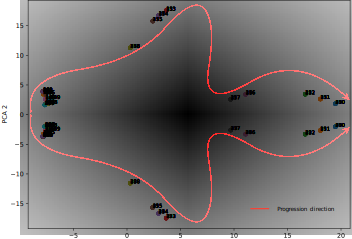
\includegraphics[width=0.8\linewidth]{figures/overcooked_figures/transition_pca.pdf}
    \caption{PCA of transition trajectories in Overcooked-AI}
    \label{fig:overcooked_pca}
\end{figure}

\

These results confirm that \textbf{MAMAD} improves toy-environment outcomes by speeding convergence, increasing robustness, and enhancing explainability. \textbf{Soft constraints} balance performance and compliance, \textbf{hard constraints} increase discipline at the cost of some reward, and omitting constraints yields fragile, less interpretable behaviors.

\paragraph*{Consistency across agents (G3).}
The consistency score ($S_{cons}$) quantifies the extent to which agents sharing
the same role behave similarly across trajectories. Consistency is lowest for RB
($55$ to $65\%$) and markedly higher for OB ($82$ to $90\%$). MB closely matches or
exceeds OB ($88$ to $93\%$) because role-aligned behavior emerges directly from the
training dynamics, and Auto-TEMM reinforces these patterns by pruning noisy or
spurious behaviors.

\paragraph*{Environment-level differences.}
The level of explainability varies across environments:

\begin{itemize}
    \item \textbf{Warehouse Management} shows the highest $F_{org}$ and $S_{cons}$
          due to its deterministic and hierarchically structured workflow.
    \item \textbf{Overcooked-AI} yields high consistency but slightly lower fit, as
          players' roles have overlapping responsibilities that can lead to rule
          ambiguity.
    \item \textbf{Predator-Prey} exhibits lower explainability due to strategic
          symmetry and interchangeable roles, which complicates rule extraction.
    \item \textbf{Drone Swarm} yields high interpretability because organizational
          structure (Analyst, Firewall, Operator) strongly matches functional network
          responsibilities.
\end{itemize}

Overall, MB offers a compelling combination of structural integrity and adaptive
learning, supporting both G2 (compliance with symbolic expectations) and G3
(explainability through interpretable artifacts extracted from trajectories).



\section{Conclusion and perspectives}\label{sec:conclusion}

This work introduced \textbf{MAMAD}, a method for automating the design of multi-agent systems by integrating organizational modeling with MARL. By structuring the design process into distinct phases (environment modeling, agent training, behavior analysis, and deployment) MAMAD reduces reliance on expert intervention while increasing automation throughout the MAS development workflow. Quantitative evaluations show that MAMAD not only accelerates design iterations but also improves compliance with organizational constraints and enhances the explainability of agent roles and missions. These results underscore the potential of combining MARL with organizational frameworks to streamline and strengthen MAS development.

While MAMAD offers a structured and automated workflow for MAS design, it still presents several limitations that warrant further research. Expert oversight remains necessary for defining reward functions and tuning hyperparameters; the method's scalability to complex, large-scale, or real-world settings remains limited; interpretability of learned behaviors, especially in adversarial contexts, could be enhanced; and the computational overhead of automated modeling may hinder real-time applications. Finally, we emphasize that while MAMAD is an attempt to automate MAS design, it is not intended to replace general-purpose AOSE methodologies.

Additionally, the TEMM method does not explicitly prescribe planning structures as found in BDI architectures. A promising direction for extending MAMAD is therefore to incorporate plan-level reasoning. First, \textit{plan-guided learning} could leverage symbolic plan templates to guide the decomposition of complex goals into structured sub-goals during MARL training, rather than relying solely on flat reward engineering. Second, \textit{plan extraction from learned behavior} could be achieved by analyzing recurrent patterns in joint-observation trajectories to identify latent sequences of sub-goals, alternatives, or parallelizable actions.
Those future works may also benefit from integrating advanced interpretability tools such as causal reasoning or attention-based visualizations, improving scalability to high-dimensional problems and large agent populations, combining automation with human-in-the-loop feedback to balance control and flexibility, and validating MAMAD in real-world domains like robotics, cybersecurity, or logistics.

Beyond these general directions, future research will focus on strengthening each step of the MAMAD workflow: modeling will integrate neuro-symbolic representations into multi-agent world models to better encode organizational constraints directly in latent dynamics, studying how symbolic roles and goals can shape latent representations and help maintain consistency between symbolic organizational models and learned world models; training will explore extensions such as formal verification of emergent behaviors using role-based hard constraints, hierarchical role structures where roles and sub-goals possess weighted priorities, and training signals that better reflect organizational semantics; analysis will investigate approaches to extract robust symbolic descriptions from learned behaviors, including leveraging large language models to semantically interpret clusters of transitions, generate human-readable role descriptions, and identify latent goal structures; and transfer will address maintaining coherence between simulation (reality conditions by studying mechanisms to detect simulation) reality divergence, trigger incremental retraining of both the world model and policies, and ensure long-term behavioral consistency during deployment. Together, these directions support the development of a more unified, end-to-end MAS engineering framework combining symbolic AOSE principles with automated data-driven learning.

\section*{Declarations}
%
\begin{enumerate*}
    \item \textbf{Funding:} This work was supported by Thales Land \& Air Systems.
    \item \textbf{Conflict of interest:} The authors declare no conflict of interest.
    \item \textbf{Ethics approval and consent to participate:} Not applicable.
    \item \textbf{Consent for publication:} Not applicable.
    \item \textbf{Data availability:} Not applicable.
    \item \textbf{Materials availability:} Not applicable.
    \item \textbf{Code availability:} The source code used in this study is publicly available at: \url{https://github.com/julien6/CybMASDE}
    \item \textbf{Author contributions:} Julien Soulé: conceptualization, methodology, implementation, writing--original draft.\\
    Jean-Paul Jamont, Michel Occello: supervision, writing--review.\\
    Louis-Marie Traonouez, Paul Théron: validation, writing--review.
\end{enumerate*}

\setlength{\bibsep}{4.5pt}
\bibliography{references}

\end{document}
